%%%%%%%%%%%%%%%%%%%%%%%%%%%%%%%%%%%%%%%%%%%%%%%%%%%%%%%%%%%%%%%%%%%%%%%%%%%%%%%%
%%%%%%%%%%%%%%%%%%%%%%%%%%%%%%%%%%%%%%%%%%%%%%%%%%%%%%%%%%%%%%%%%%%%%%%%%%%%%%%%
%%%%%%%%%%%%%%%%%%%%%%%%%%%%%%%%%%%%%%%%%%%%%%%%%%%%%%%%%%%%%%%%%%%%%%%%%%%%%%%%
%%%%%%%%%%%%%%%%%%%%%%%%%%%%%%%%%%%%%%%%%%%%%%%%%%%%%%%%%%%%%%%%%%%%%%%%%%%%%%%%
\chapter{Stabilité des systèmes asservis\label{chap-stab}}
%%%%%%%%%%%%%%%%%%%%%%%%%%%%%%%%%%%%%%%%%%%%%%%%%%%%%%%%%%%%%%%%%%%%%%%%%%%%%%%%
%%%%%%%%%%%%%%%%%%%%%%%%%%%%%%%%%%%%%%%%%%%%%%%%%%%%%%%%%%%%%%%%%%%%%%%%%%%%%%%%
%%%%%%%%%%%%%%%%%%%%%%%%%%%%%%%%%%%%%%%%%%%%%%%%%%%%%%%%%%%%%%%%%%%%%%%%%%%%%%%%
%%%%%%%%%%%%%%%%%%%%%%%%%%%%%%%%%%%%%%%%%%%%%%%%%%%%%%%%%%%%%%%%%%%%%%%%%%%%%%%%
\minitoc
\newpage
%%%%%%%%%%%%%%%%%%%%%%%%%%%%%%%%%%%%%%%%%%%%%%%%%%%%%%%%%%%%%%%%%%%%%%%%%%%%%%%%
%%%%%%%%%%%%%%%%%%%%%%%%%%%%%%%%%%%%%%%%%%%%%%%%%%%%%%%%%%%%%%%%%%%%%%%%%%%%%%%%
%%%%%%%%%%%%%%%%%%%%%%%%%%%%%%%%%%%%%%%%%%%%%%%%%%%%%%%%%%%%%%%%%%%%%%%%%%%%%%%%
\section{Contexte et définition de la stabilité} 
%%%%%%%%%%%%%%%%%%%%%%%%%%%%%%%%%%%%%%%%%%%%%%%%%%%%%%%%%%%%%%%%%%%%%%%%%%%%%%%%
%%%%%%%%%%%%%%%%%%%%%%%%%%%%%%%%%%%%%%%%%%%%%%%%%%%%%%%%%%%%%%%%%%%%%%%%%%%%%%%%
%%%%%%%%%%%%%%%%%%%%%%%%%%%%%%%%%%%%%%%%%%%%%%%%%%%%%%%%%%%%%%%%%%%%%%%%%%%%%%%%
Dans ce chapitre nous allons étudier en détail la stabilité des systèmes
linéaires asservis. Il faut dors et déjà noter que ce sont les états 
d'équilibres\footnote{(ou point fixes). Un état d'équilibre est une constante
solution de l'équation différentielle du système. En générale, 0 est toujours
une solution de l'équation différentielle et donc considéré comme l'état 
d'équilibre du système} qui sont stables ou instables et non les systèmes eux 
mêmes. Cet \og abus de langage\fg (largement utilisé) provient du fait que 
on considère \emph{a priori} les systèmes dans leur état d'équilibre 
au moment de l'instant initial de la sollicitation. 
Une façon de se représenter ces états d'équilibres est d'imaginer le 
mouvement d'une bille à la surface d'une fonction d'energie potentielle à une 
dimension. 
On peut facilement généraliser à plusieurs dimensions, en considérant le 
déplacement de la bille sur un relief accidenté et composé de collines, 
vallées ou puits à l'image d'un paysage d'énergie potentielle 
(c.f \Cref{fig-stab}). L'état d'équilibre de la bille est donc ici 
une position d'équilibre.
%-------------------------------------------------------------------------------
\begin{figure}[!h]
    \centering
    \tikzsetnextfilename{stable_1-chap_stab-ext}
    \begin{tikzpicture}
    \draw[col3,line width=0.5mm] (0,0.25) circle (1.5ex);
    \draw[thick] (0,0) parabola (1,1.75) ;
    \draw[thick] (0,0) parabola (-1,1.75) ;
    \node at (0,-2.5) {(a) stable};
    \begin{scope}[xshift=3.5cm]
        \draw[col4,line width=0.5mm] (0,0.25) circle (1.5ex);
        \draw[thick] (0,0) parabola (1,-1.75) ;
        \draw[thick] (0,0) parabola (-1,-1.75) ;
        \node at (0,-2.5) {(b) instable};
    \end{scope}
    \begin{scope}[xshift=7cm]
        \draw[col1,line width=0.5mm] (0,0.25) circle (1.5ex);
        \draw[thick] (0,0) parabola (-1,1.75) ;
        \draw[thick] (0,0) parabola (0.5,0.2) ;
        \draw[thick] (0.5,0.2) parabola (1,-1.75) ;
        \node[text width=3cm,align=center] at (0,-2.5) 
        {(c) stabilité\\conditionnelle};
    \end{scope}
\end{tikzpicture}

    \caption{Représentation schématique de la stabilité d'un équilibre
             \label{fig-stab}}
\end{figure}
%-------------------------------------------------------------------------------

La manière la plus simple de caractériser la stabilité de ces positions 
d'équilibres c'est de s'en écarter. 
Dans le cas d'un équilibre stable 
(c.f \Cref{fig-stab} (a)), la bille va naturellement reprendre sa position 
d'équilibre (avec ou sans oscillations autour de la position d'équilibre). 
Dans le cas d'un équilibre instable, 
(c.f \Cref{fig-stab} (b)), la bille va continuer à s'en écarter indéfiniment. 
D'autres scénarios sont possibles mais vont dépendre de la façon dont le 
système est déséquilibré et de la forme de la surface d'énergie potentielle 
(c.f \Cref{fig-stab} (c)). On parle alors de stabilité conditionnelle.

Dans le cas des \gls{slci}, il est possible d'étudier la stabilité du système 
en étudiant sa réponse impulsionnelle (l'impulsion de Dirac permet d'écarter 
le système de son état d'équilibre dans lequel il se trouvait). 
Finalement, on définit la stabilité d'un système de la façon 
suivante :
%-------------------------------------------------------------------------------
\begin{definition}{Définition : Stabilité d'un système (1)}
Un système est dit stable lorsque écarté de son état d'équilibre, il 
tend à y revenir
\end{definition}
%-------------------------------------------------------------------------------
Il existe une autre définition de la stabilité qui s'avère équivalente 
dans le cas des systèmes linéaires.
%-------------------------------------------------------------------------------
\begin{definition}{Définition : Stabilité d'un système (2)}
\textbf{Un système est dit stable si à une entrée bornée le système produit 
une sortie bornée}
\end{definition}
%-------------------------------------------------------------------------------
En anglais, on rencontre l'acronyme \gls{bibo}
pour désigner cette notion.
Ci-dessous nous avons représenté les réponses de \gls{slci} à différentes
sollicitations bornées. D'après la définition précédente, il est aisé
de caractériser la stabilité de ces systèmes en observant la forme de la 
réponse.
%-------------------------------------------------------------------------------
\begin{figure}[!t]
    \centering
    \tikzsetnextfilename{stabilite-bibo-chap_stab_ext}
    \pgfmathdeclarefunction{func}{1}{%
    \pgfmathparse{%
    1-((1./sqrt(1-#1*#1))*exp(-#1*x)*
    sin(deg(x)*sqrt(1-#1*#1)+atan(sqrt(1-#1*#1)/#1)))
    }%
}
\begin{tikzpicture}
    \begin{scope}[yshift=4.5cm]
        \begin{axis}
        [
            xtick=\empty,
            height=3.7cm,
            width=5.5cm,
            xmin=-1,xmax=5,
            ymin=-0.5,ymax=1.25,
            axis x line=center,
            axis y line=center,
            xlabel style={below},
            ylabel style={above left},
            xlabel=$t$,
            ylabel={\textcolor{col1}{$e(t)$}},
            tick label style={color=col1,font=\scriptsize},
            yticklabels={$E_0$},
            ytick={1},
            clip=false
        ]
            \addplot+[col1,thick,mark=none,const plot]
            coordinates
            {(-1,0) (0,0) (0,1) (1,1) (5,1)};
        \end{axis}
    \end{scope}
    \begin{scope}[yshift=1.5cm]
        \begin{axis}
        [
            xtick=\empty,
            height=3.7cm,
            width=5.5cm,
            xmin=-1,xmax=5,
            ymin=-0.5,ymax=1.25,
            axis x line=center,
            axis y line=center,
            xlabel style={below},
            ylabel style={above left},
            xlabel=$t$,
            ylabel={\textcolor{col1}{$e(t)$}},
            tick label style={color=col1,font=\scriptsize},
            yticklabels={$E_0$},
            ytick={1},
            clip=false
        ]
            \addplot+[col1,thick,mark=none,const plot]
            coordinates
            {(-1,0) (0,0) (0,1) (1,0) (5,0)};
        \end{axis}
    \end{scope}
    \begin{scope}[yshift=-1.5cm]
        \begin{axis}
        [
            xtick=\empty,
            height=3.7cm,
            width=5.5cm,
            xmin=-4,xmax=20,
            ymin=-1.25,ymax=1.25,
            axis x line=center,
            axis y line=center,
            xlabel style={below},
            ylabel style={above left},
            xlabel=$t$,
            ylabel={\textcolor{col1}{$e(t)$}},
            tick label style={color=col1,font=\scriptsize},
            yticklabels={$E_0$},
            ytick={1},
        ]
            \addplot[col1,thick,samples=100,domain=-4:0] {0};
            \addplot[col1,thick,samples=100,domain=0:20] {sin(deg(x))};
        \end{axis}
    \end{scope}
    \begin{scope}[xshift=4.75cm,yshift=-0.5cm]
        \bs[\textcolor{col1}{$E(p)$}][$H_1(p)$][][\textcolor{col4}{$S(p)$}]
    \end{scope}
    \begin{scope}[xshift=4.75cm,yshift=2cm]
        \bs[\textcolor{col1}{$E(p)$}][$H_2(p)$][][\textcolor{col4}{$S(p)$}]
    \end{scope}
    \begin{scope}[xshift=4.75cm,yshift=5cm]
        \bs[\textcolor{col1}{$E(p)$}][$H_3(p)$][][\textcolor{col4}{$S(p)$}]
    \end{scope}
    \begin{scope}[xshift=10cm,yshift=4.5cm]
        \begin{axis}
        [
            xtick=\empty,
            height=3.7cm,
            width=5.5cm,
            xmin=-1,xmax=15,
            ymin=-0.5,ymax=1.75,
            axis x line=center,
            axis y line=center,
            xlabel style={below},
            ylabel style={above left},
            xlabel=$t$,
            ylabel={\textcolor{col4}{$s(t)$}},
            tick label style={color=col4,font=\scriptsize},
            yticklabels={$KE_0$},
            ytick={1},
        ]
            \addplot[col4,thick,samples=100,mark=none,domain=0:15] {func(0.25)};
        \end{axis}
    \end{scope}
    \begin{scope}[xshift=10cm,yshift=1.5cm]
        \begin{axis}
        [
            xtick=\empty,
            height=3.7cm,
            width=5.5cm,
            xmin=-0.3,xmax=4,
            ymin=-0.5,ymax=1.25,
            axis x line=center,
            axis y line=center,
            xlabel style={below},
            ylabel style={above left},
            xlabel=$t$,
            ylabel={\textcolor{col4}{$s(t)$}},
            tick label style={color=col4,font=\scriptsize},
            yticklabels={$KE_0$},
            ytick={1},
        ]
            \addplot[col4,thick,samples=100,mark=none,domain=0:1] {1-exp(-x/0.25)};
            \addplot[col4,thick,samples=100,mark=none,domain=1:5] {(-exp(-x/0.25)+exp(-(x-1)/0.25)};
        \end{axis}
    \end{scope}
    \begin{scope}[xshift=10cm,yshift=-1.5cm]
        \begin{axis}
        [
            xtick=\empty,
            height=3.7cm,
            width=5.5cm,
            xmin=-1.33,xmax=20,
            ymin=-1.25,ymax=1.25,
            axis x line=center,
            axis y line=center,
            xlabel style={below},
            ylabel style={above left},
            xlabel=$t$,
            ylabel={\textcolor{col4}{$s(t)$}},
            tick label style={color=col4,font=\scriptsize},
            yticklabels={$KE_0$},
            ytick={1},
        ]
            \addplot[col4,thick,samples=100,mark=none,domain=0:20] {0.8*sin(deg(x)-90)};
        \end{axis}
    \end{scope}
\end{tikzpicture}

    \caption{Exemples de systèmes (vert) stables et (rouge) instables. Les 
    systèmes stables présentent une réponse bornée à une sollicitation elle-même
    bornée.}
\end{figure}
%-------------------------------------------------------------------------------
\newpage
%%%%%%%%%%%%%%%%%%%%%%%%%%%%%%%%%%%%%%%%%%%%%%%%%%%%%%%%%%%%%%%%%%%%%%%%%%%%%%%%
%%%%%%%%%%%%%%%%%%%%%%%%%%%%%%%%%%%%%%%%%%%%%%%%%%%%%%%%%%%%%%%%%%%%%%%%%%%%%%%%
%%%%%%%%%%%%%%%%%%%%%%%%%%%%%%%%%%%%%%%%%%%%%%%%%%%%%%%%%%%%%%%%%%%%%%%%%%%%%%%%
\section[Instabilité de l'asservissement]
{Mise en évidence de l'instabilité de l'asservissement}
%%%%%%%%%%%%%%%%%%%%%%%%%%%%%%%%%%%%%%%%%%%%%%%%%%%%%%%%%%%%%%%%%%%%%%%%%%%%%%%%
%%%%%%%%%%%%%%%%%%%%%%%%%%%%%%%%%%%%%%%%%%%%%%%%%%%%%%%%%%%%%%%%%%%%%%%%%%%%%%%%
%%%%%%%%%%%%%%%%%%%%%%%%%%%%%%%%%%%%%%%%%%%%%%%%%%%%%%%%%%%%%%%%%%%%%%%%%%%%%%%%
\index{Instabilité des systèmes asservis! phénomène de pompage}
\index{Phénomène de pompage}
Nous avons vu au~\cref{chap-asservis} que l'asservissement permettait de
rendre stable un système intrinsèquement instable. C'est le cas notamment d'un 
intégrateur pur qui lorsque placé dans une boucle de contre-réaction devient
un système du premier ordre.
Cependant, l'asservissement peut également rendre un système instable par
bouclage, on parle alors de \textbf{phénomène de pompage}.
Pour illustrer ce phénomène\cite{genouel}, considérons un système de fonction 
de transfert d'un retard pur $H(p)=Ke^{-p\frac{\tau}{2}}$ qui entraîne 
un déphasage de $\tau/2$ et de gain $K$. Si on sollicite ce système par un 
signal $e(t)$ rectangulaire de période $\tau$ et d'amplitude $E_0$, la sortie 
est de même nature et est donc simplement amplifiée de $K$ et déphasée 
de $\tau/2$, comme représentée ci-dessous.
%-------------------------------------------------------------------------------
\begin{center}
    \tikzsetnextfilename{instabilite_pompage-non_boucle-chap_stab_ext}
    \begin{tikzpicture}
    \begin{scope}[baseline=0pt]
        \begin{axis}
        [
            xtick=\empty,
            height=3.7cm,
            width=5.5cm,
            xmin=-1,xmax=7,
            ymin=-2.5,ymax=2.5,
            axis x line=center,
            axis y line=center,
            xlabel style={below},
            ylabel style={above left},
            xlabel=$t$,
            ylabel={\textcolor{col1}{$e(t)$}},
            tick label style={color=col1,font=\scriptsize},
            yticklabels={$E_0$},
            ytick={1},
            clip=false
        ]
            \addplot+[col1,thick,mark=none,const plot]
            coordinates
            {(-1,0) (0,0) (0,1) (1,-1) (2,1) (3,-1) (4,1) (5,-1) (6,1) (7,1)};
        \end{axis}
    \end{scope}
    \begin{scope}[xshift=4.75cm,yshift=1cm]
        \bs[\textcolor{col1}{$E(p)$}][$H(p)$][][\textcolor{col3}{$S(p)$}]
    \end{scope}
    \begin{scope}[xshift=10cm]
        \begin{axis}
        [
            xtick=\empty,
            height=3.7cm,
            width=5.5cm,
            xmin=-1,xmax=7,
            ymin=-2.5,ymax=2.5,
            axis x line=center,
            axis y line=center,
            xlabel style={below},
            ylabel style={above left},
            xlabel=$t$,
            ylabel={\textcolor{col3}{$s(t)$}},
            tick label style={color=col3,font=\scriptsize},
            yticklabels={$KE_0$},
            ytick={1.5},
            xticklabels={$\dfrac{\tau}{2}$},
            xtick={1},
            clip=false
        ]
            \addplot+[col3,thick,mark=none,const plot]
            coordinates
            {(-1,0) (1,0) (1,1.5) (2,-1.5) (3,1.5) 
             (4,-1.5) (5,1.5) (6,-1.5) (7,-1.5)};
        \end{axis}
    \end{scope}
\end{tikzpicture}

\end{center}
%-------------------------------------------------------------------------------
Si on place maintenant ce système dans une boucle de contre-réaction 
unitaire le système est alors soumis à la différence entre les signaux 
d'entrée et de sortie $\epsilon(t)=e(t)-s(t)$. 
%-------------------------------------------------------------------------------
\begin{center}
    \tikzsetnextfilename{instabilite_pompage-chap_stab_ext}
    \begin{tikzpicture}
    \begin{scope}[baseline=0pt]
        \begin{axis}
        [
            xtick=\empty,
            height=3.7cm,
            width=5.5cm,
            xmin=-1,xmax=7,
            ymin=-2.5,ymax=2.5,
            axis x line=center,
            axis y line=center,
            xlabel style={below},
            ylabel style={above left},
            xlabel=$t$,
            ylabel={\textcolor{col1}{$e(t)$}},
            tick label style={color=col1,font=\scriptsize},
            yticklabels={$E_0$},
            ytick={1},
            clip=false
        ]
            \addplot+[col1,thick,mark=none,const plot]
            coordinates
            {(-1,0) (0,0) (0,1) (1,-1) (2,1) (3,-1) (4,1) (5,-1) (6,1) (7,1)};
        \end{axis}
    \end{scope}
    \begin{scope}[scale=0.6, every node/.append style={transform shape},
                  xshift=7.5cm,yshift=2cm]
        \bruni[\textcolor{col1}{$E(p)$}]
              [\textcolor{col5}{$\epsilon(p)$}]
              [$H(p)$]
              []
              [\textcolor{col4}{$S(p)$}]
    \end{scope}
    \begin{scope}[xshift=10cm]
        \begin{axis}
        [
            xtick=\empty,
            ytick=\empty,
            height=3.7cm,
            width=5.5cm,
            xmin=-1,xmax=7,
            ymin=-12.5,ymax=7.5,
            axis x line=center,
            axis y line=center,
            xlabel style={below},
            ylabel style={above left},
            xlabel=$t$,
            ylabel={\textcolor{col4}{$s(t)$}},
            tick label style={color=col4,font=\scriptsize},
            yticklabels={$s_1$,$s_2$,$s_3$,$s_4$,$s_5$},
            ytick={1.5,-3.75,7.125,-12.1875,19.78125},
            clip=false
        ]
            \addplot+[col4,thick,mark=none,const plot]
            coordinates
            {(-1,0) (1,0) (1,1.5) (2,-3.75) (3,7.125) (4,-12.1875) 
             (5,19.78125) (6,19.78125) };
        \end{axis}
    \end{scope}
    \begin{scope}[xshift=4.75cm,yshift=3.25cm]
        \begin{axis}
        [
            xtick=\empty,
            ytick=\empty,
            height=3.7cm,
            width=5.5cm,
            xmin=-1,xmax=7,
            ymin=-12.5,ymax=7.5,
            axis x line=center,
            axis y line=center,
            xlabel style={below},
            ylabel style={above left},
            xlabel=$t$,
            ylabel={\textcolor{col5}{$\epsilon(t)$}},
            tick label style={color=col5,font=\scriptsize},
            yticklabels={$\epsilon_1$,$\epsilon_2$,$\epsilon_3$,
                         $\epsilon_4$,$\epsilon_5$},
            ytick={1,-2.5,4.75,-8.125,13.1875,-20.78125},
            clip=false
        ]
            \addplot+[col5,thick,mark=none,const plot]
            coordinates
            {(-1,0) (0,1.0) (1,-2.5) (2,4.75) (3,-8.125) 
             (4,13.1875) (5,-20.78125)  (6,-20.78125) };
        \end{axis}
    \end{scope}
\end{tikzpicture}

\end{center}
%-------------------------------------------------------------------------------
Nous allons établir la relation 
entre les valeurs des signaux par demi-période $\tau/2$. 
\[
    \epsilon_i=e_i-s_i
\]
où $\epsilon_i$, $e_i$ et $s_i$ sont respectivement les valeurs des signaux 
$\epsilon(t)$, $e(t)$ et $s(t)$ pour la demi-période $i\in[1,+\infty]$
Dans cette notation, la sortie du système bouclé est donnée par : 
\[
    s_{i+1}=K\epsilon_i
\]
Pour la première demi-période, la sollicitation est positive $e_1=E_0$, 
le système étant causal ($\epsilon_0=0$), on a $s_1=0$ et donc $\epsilon_1=E_0$.
Pour la seconde demi-période, la sollication est maintenant négative $e_2=-E_0$,
la sortie est maintenant donnée par $s_2=KE_0$. De la même manière pour 
la troisième demi-période, on obtient $s_3=K\epsilon_2=K(e_2-s_2)=-E_0(K+K^2)$. 
On obtient la relation suivante donnant la sortie en fonction de la 
demi-période pour $i>1$:
\[
    s_i=(-1)^{i}KE_0\sum\limits_{j=0}^{i-1} K^j
\]
La suite géométrique présente dans cette expression diverge pour $K>1$.

\textbf{Il est donc clair que l'instabilité est une conséquence de 
l'asservissement par bouclage. Il est donc essentiel d'étudier 
cette propriété dans le cas des systèmes asservis.}
Il faut cependant noter l'influence indispensable du :
\begin{itemize}
    \item gain statique en boucle ouverte $K>1$
    \item et du retard d'une demi-période (en opposition de phase); 
\end{itemize}
dans cet exemple. Comme attendu, les propriétés de la boucle ouverte
influencent directement la stabilité de la boucle fermée.
%%%%%%%%%%%%%%%%%%%%%%%%%%%%%%%%%%%%%%%%%%%%%%%%%%%%%%%%%%%%%%%%%%%%%%%%%%%%%%%%
%%%%%%%%%%%%%%%%%%%%%%%%%%%%%%%%%%%%%%%%%%%%%%%%%%%%%%%%%%%%%%%%%%%%%%%%%%%%%%%%
%%%%%%%%%%%%%%%%%%%%%%%%%%%%%%%%%%%%%%%%%%%%%%%%%%%%%%%%%%%%%%%%%%%%%%%%%%%%%%%%
\section[Condition fondamentale de stabilité]
{Condition fondamentale de stabilité d'un système asservis}
%%%%%%%%%%%%%%%%%%%%%%%%%%%%%%%%%%%%%%%%%%%%%%%%%%%%%%%%%%%%%%%%%%%%%%%%%%%%%%%%
%%%%%%%%%%%%%%%%%%%%%%%%%%%%%%%%%%%%%%%%%%%%%%%%%%%%%%%%%%%%%%%%%%%%%%%%%%%%%%%%
%%%%%%%%%%%%%%%%%%%%%%%%%%%%%%%%%%%%%%%%%%%%%%%%%%%%%%%%%%%%%%%%%%%%%%%%%%%%%%%%
Pour caractériser la stabilité des \gls{slci}, il est possible de déterminer
une condition sur les p ôles (racines du dénominateur de la fonction de 
transfert). Pour montrer cela, nous allons étudier la réponse impulsionnelle 
d'une fonction de transfert présentant des pôles de différentes natures et oberver
la condition sur ses pôles pour que le système soit stable selon les définitions
précédentes. 
Soit une fonction de transfert $H(p)$ présentant quatre pôles :
\begin{itemize}
    \item un pôle réel simple $p_1$,
    \item un pôle réel double $p_2$,
    \item deux pôles complexes conjugués $p_{3,4}=\alpha\pm\jw$
\end{itemize}
tel que :
\[
    H(p)=\dfrac{N(p)}{(p-p_1)(p-p_2)^2(p-p_3)(p-p_4)}.
\]
En notant que $(p-p_3)(p-p_4)=(p-\alpha)^2+\omega^2$, 
la décomposition en élément simple de la réponse impulsionnelle $S(p)$ 
dans le domaine de Laplace devient :
\[
    S(p)=\dfrac{A}{p-p_1}+\dfrac{B}{p-p_2}+\dfrac{C}{(p-p_2)^2}+\dfrac{Dp+E}{(p-\alpha)^2+\omega^2}
\]
La transformée inverse de cette expression est de la forme:
\[
    s(t)=\left(Ae^{p_1t}+=Be^{p_2t}+Cte^{p_2t}+De^{\alpha t}\cos{\omega t}+\dfrac{\alpha D+E}{\alpha}e^{\alpha t}\sin{\omega t}\right)u(t)
\]
Il apparaît clair que les pôles doivent être à parties réelles strictement 
négatives pour que les exponentielles présentent dans la réponse temporelle
tendent vers 0 pour $t\to0$.
%-------------------------------------------------------------------------------
\clearpage
\thispagestyle{empty}
\begin{landscape}
\centering
\captionsetup{width=1.10\linewidth}
%-------------------------------------------------------------------------------
\begin{figure}[!h]
    \centering
    \tikzsetnextfilename{stabilite_plan-complexe-chap_stab_ext}
    \clearpage
\thispagestyle{empty}
\begin{landscape}
    \centering
    %\vspace*{\fill}
    \captionsetup{width=1.15\linewidth}
    \begin{figure}[!h]
        \centering
        \begin{tikzpicture}
        \begin{axis}[                                                                                                                     ticks=none,
            width=1.6\textheight,           
            height=\textwidth,    
            axis x line=center,                                                                            
            axis y line=center,
            xmin=-12.5,                                                                                                  
            xmax=12.5,
            ymin=-5,                                                                                                         
            ymax=5,
            xlabel={\LARGE $\Re{(p)}$},
            ylabel={\LARGE $\Im{(p)}$},
            xlabel style={right},
            ylabel style={above},                                                                                       
            ]      
            \draw [white!90!blue,fill=white!95!blue]   (axis cs:-12.5,-5) rectangle (axis cs:0,5);
            \draw [white!90!black,fill=white!90!black] (axis cs:0,-5) rectangle (axis cs:12.5,5);

            \draw [ultra thick,-latex]   (axis cs:-12.5,0) -- (axis cs:12.5,0);
            \draw [ultra thick,-latex]   (axis cs:0,-5) -- (axis cs:0,5);

            \coordinate (pt01) at (axis cs:-6.5,4.5);
            \coordinate (pt02) at (axis cs:6.5,4.5);

            \coordinate (pt1) at (axis cs:-12.5,2.0);
            \addplot[mark=x,black!60!green,ultra thick,only marks,mark size=7pt]  coordinates{ (-11,1.5) (-11,-1.5) } ;      
            \draw[ultra thick,dotted,color=black!60!green] (axis cs:-11,1.5) -- (axis cs:-11,-1.5) ;

            \coordinate (pt2) at (axis cs:-7,1.0);
            \addplot[mark=x,black!10!green,ultra thick,only marks,mark size=7pt]  coordinates{ (-5,0.5) (-5,-0.5) } ;  
            \draw[ultra thick,dotted,color=black!10!green] (axis cs:-5,0.5) -- (axis cs:-5,-0.5) ;

            \coordinate (pt3) at (axis cs:-10.25,-3.0);
            \addplot[mark=x,black!50!red,ultra thick,only marks,mark size=7pt]    coordinates{ (-8,0) } ;             

            \coordinate (pt4) at (axis cs:-4.75,-3.0);
            \addplot[mark=x,red,ultra thick,only marks,mark size=7pt]    coordinates{ (-2,0) } ;                      

            \coordinate (pt5) at  (axis cs:1.25,-5);
            \coordinate (pt52) at (axis cs:1.25,-3);
            \addplot[mark=x,black,ultra thick,only marks,mark size=7pt]  coordinates{ (0,0) } ;                      

            \coordinate (pt6) at (axis cs:1.25,2);
            \coordinate (pt62) at (axis cs:1.25,0);
            \addplot[mark=x,black!50!white,ultra thick,only marks,mark size=7pt]  coordinates{ (0,2) (0,-2) } ;              
            \draw[ultra thick,dotted,color=black!50!white] (axis cs:0,-2) to[bend right] (axis cs:0,2);

            \coordinate (pt7) at (axis cs:8.25,2);
            \addplot[mark=x,blue,ultra thick,only marks,mark size=7pt]   coordinates{ (11,1.5) (11,-1.5) } ;                
            \draw[ultra thick,dotted,color=blue] (axis cs:11,1.5) -- (axis cs:11,-1.5) ;

            \coordinate (pt8) at (axis cs:6.5,-3);
            \addplot[mark=x,orange,ultra thick,only marks,mark size=7pt] coordinates{ (8,0) } ;                  

        \end{axis}


            \node at (pt01) {\textbf{\Large STABLE}};
            \node at (pt02) {\textbf{\Large INSTABLE}};
            % pt1
            \node[anchor=south west] at (pt1) {
                \begin{tikzpicture}
                    \begin{axis}[
                    ticks=none,
                    width=4cm,    
                    height=4cm,    
                    axis x line=center,                                                                            
                    axis y line=center,
                    xmin=-0.5,                                                                                                                    xmax=6.5,
                    ymin=-0.5,                                                                        
                    ymax=2.5,
                    xlabel={$t$},
                    ylabel={$s(t)$},
                    xlabel style={below right},
                    ylabel style={right}
                    ]
                    \addplot [very thick,color=black!60!green,domain=0:10, samples=501,unbounded coords=jump]{1.2*sin(4.5*deg(x))*exp(-0.7*x)};
                    \addplot [thick,dotted,color=black,domain=0:10, samples=501,unbounded coords=jump]{1.2*exp(-0.7*x)+1};
                    \addplot [thick,dotted,color=black,domain=0:10, samples=501,unbounded coords=jump]{-1.2*exp(-0.7*x)+1};
                    \end{axis}
                \end{tikzpicture}
            };

            % pt2
            \node[anchor=south west] at (pt2) {
                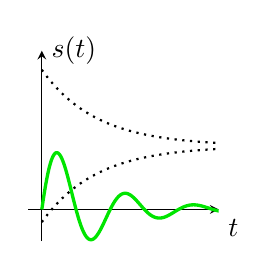
\begin{tikzpicture}
                    \begin{axis}[
                    ticks=none,
                    width=4cm,    
                    height=4cm,    
                    axis x line=center,                                                                            
                    axis y line=center,
                    xmin=-0.5,                                                                                                                    xmax=6.5,
                    ymin=-0.5,                                                                        
                    ymax=2.5,
                    xlabel={$t$},
                    ylabel={$s(t)$},
                    xlabel style={below right},
                    ylabel style={right}
                    ]
                    \addplot [very thick,color=black!10!green,domain=0:10, samples=501,unbounded coords=jump]{1.2*sin(2.5*deg(x))*exp(-0.5*x)};
                    \addplot [thick,dotted,color=black,domain=0:10, samples=501,unbounded coords=jump]{1.2*exp(-0.5*x)+1};
                    \addplot [thick,dotted,color=black,domain=0:10, samples=501,unbounded coords=jump]{-1.2*exp(-0.5*x)+1};
                    \end{axis}
                \end{tikzpicture}
            };
            % pt3
            \node[anchor=south west] at (pt3) {
                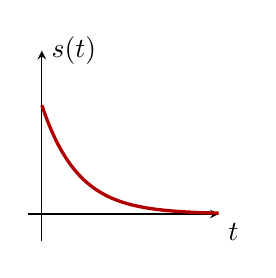
\begin{tikzpicture}
                    \begin{axis}[
                    ticks=none,
                    width=4cm,    
                    height=4cm,    
                    axis x line=center,                                                                            
                    axis y line=center,
                    xmin=-0.5,                                                                                                                    xmax=6.5,
                    ymin=-0.5,                                                                        
                    ymax=3,
                        xlabel={$t$},
                        ylabel={$s(t)$},
                    xlabel style={below right},
                    ylabel style={right}
                    ]
                    \addplot [very thick,color=black!30!red,domain=0:10, samples=501,unbounded coords=jump]{2*exp(-0.75*x)};
                    \end{axis}
                \end{tikzpicture}
            };
            % pt4
            \node[anchor=south west] at (pt4) {
                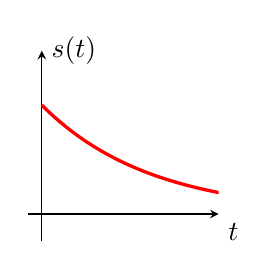
\begin{tikzpicture}
                    \begin{axis}[
                    ticks=none,
                    width=4cm,    
                    height=4cm,    
                    axis x line=center,                                                                            
                    axis y line=center,
                    xmin=-0.5,                                                                                                                    xmax=6.5,
                    ymin=-0.5,                                                                        
                    ymax=3,
                        xlabel={$t$},
                        ylabel={$s(t)$},
                    xlabel style={below right},
                    ylabel style={right}
                    ]
                    \addplot [very thick,color=red,domain=0:10, samples=501,unbounded coords=jump]{2*exp(-0.25*x)};
                    \end{axis}
                \end{tikzpicture}
            };
            % pt5
            \node[anchor=south west] at (pt5) {
                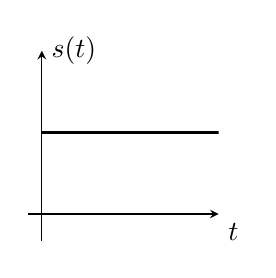
\begin{tikzpicture}
                    \begin{axis}[
                    ticks=none,
                    width=4cm,    
                    height=4cm,    
                    axis x line=center,                                                                            
                    axis y line=center,
                    xmin=-0.5,                                                                                                                    xmax=6.5,
                    ymin=-0.5,                                                                        
                    ymax=3,
                    xlabel={$t$},
                    ylabel={$s(t)$},
                    xlabel style={below right},
                    ylabel style={right}
                    ]
                    \addplot [very thick,color=black,domain=0:10, samples=501,unbounded coords=jump]{1.5};
                    \end{axis}
                \end{tikzpicture}
            };
            % pt52
            \node[anchor=south west] at (pt52) {
                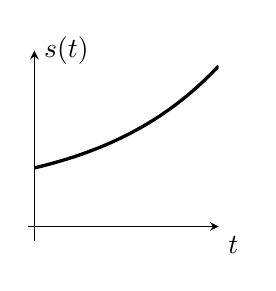
\begin{tikzpicture}
                    \begin{axis}[
                    ticks=none,
                    width=4cm,    
                    height=4cm,    
                    axis x line=center,                                                                            
                    axis y line=center,
                    xmin=-0.5,                                                                                                                    xmax=15,
                    ymin=-0.5,                                                                        
                    ymax=6,
                    xlabel={$t$},
                    ylabel={$s(t)$},
                    xlabel style={below right},
                    ylabel style={right}
                    ]
                    \addplot [very thick,color=black,domain=0:15, samples=501,unbounded coords=jump]{1+exp(0.1*x)};
                    \end{axis}
            \end{tikzpicture}
            };
            % pt6
            \node[anchor=south west] at (pt6) {
                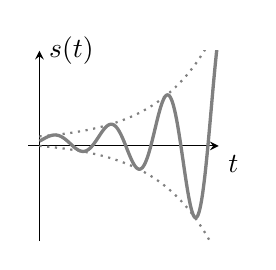
\begin{tikzpicture}
                    \begin{axis}[
                    ticks=none,
                    width=4cm,    
                    height=4cm,    
                    axis x line=center,                                                                            
                    axis y line=center,
                    xmin=-0.5,                                                                                                                    xmax=8,
                    ymin=-20,                                                                        
                    ymax=20,
                    xlabel={$t$},
                    ylabel={$s(t)$},
                    xlabel style={below right},
                    ylabel style={right}
                    ]
              \addplot [very thick,color=black!50!white,domain=0:10, samples=501,unbounded coords=jump]{sin(2.5*deg(x))*exp(0.40*x)+1};
              \addplot [thick,dotted,color=black!50!white,domain=0:10, samples=501,unbounded coords=jump]{ exp(0.4*x)+1};
              \addplot [thick,dotted,color=black!50!white,domain=0:10, samples=501,unbounded coords=jump]{-exp(0.4*x)+1};
                    \end{axis}
                \end{tikzpicture}
            };
            % pt62
            \node[anchor=south west] at (pt62) {
                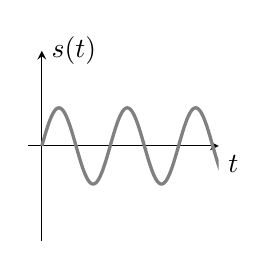
\begin{tikzpicture}
                    \begin{axis}[
                    ticks=none,
                    width=4cm,    
                    height=4cm,    
                    axis x line=center,                                                                            
                    axis y line=center,
                    xmin=-0.5,                                                                                                                    xmax=6.5,
                    ymin=-2.5,                                                                        
                    ymax=2.5,
                    xlabel={$t$},
                    ylabel={$s(t)$},
                    xlabel style={below right},
                    ylabel style={right}
                    ]
                    \addplot [very thick,color=black!50!white,domain=0:10, samples=501,unbounded coords=jump]{sin(2.5*deg(x))};
                    \end{axis}
                \end{tikzpicture}
            };
            % pt7
            \node[anchor=south west] at (pt7) {
                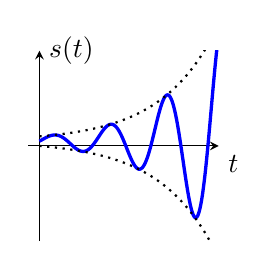
\begin{tikzpicture}
                    \begin{axis}[
                    ticks=none,
                    width=4cm,    
                    height=4cm,    
                    axis x line=center,                                                                            
                    axis y line=center,
                    xmin=-0.5,                                                                                                                    xmax=8.0,
                    ymin=-20,                                                                        
                    ymax=20,
                    xlabel={$t$},
                    ylabel={$s(t)$},
                    xlabel style={below right},
                    ylabel style={right}
                    ]
              \addplot [very thick,color=blue,domain=0:10, samples=501,unbounded coords=jump]{sin(2.5*deg(x))*exp(0.40*x)+1};
              \addplot [thick,dotted,color=black,domain=0:10, samples=501,unbounded coords=jump]{ exp(0.4*x)+1};
              \addplot [thick,dotted,color=black,domain=0:10, samples=501,unbounded coords=jump]{-exp(0.4*x)+1};
                    \end{axis}
              \end{tikzpicture}
            };
            % pt8
            \node[anchor=south west] at (pt8) {
                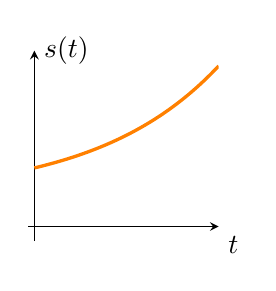
\begin{tikzpicture}
                    \begin{axis}[
                    ticks=none,
                    width=4cm,    
                    height=4cm,    
                    axis x line=center,                                                                            
                    axis y line=center,
                    xmin=-0.5,                                                                                                                    xmax=15,
                    ymin=-0.5,                                                                        
                    ymax=6,
                    xlabel={$t$},
                    ylabel={$s(t)$},
                    xlabel style={below right},
                    ylabel style={right}
                    ]
                    \addplot[very thick,color=orange,domain=0:15,samples=501,unbounded coords=jump]{1+exp(0.1*x)};
                    \end{axis}
                \end{tikzpicture}
            };
        \end{tikzpicture}
    \caption{Stabilité d'un SLCI d'après la carte des pôles de sa fonction de transfert et de leurs
    réponses impulsionnelles.
    (Vert) Deux pôles complexes conjugués. 
    (Rouge) Pôle à partie réel négative. 
    (Gris) Deux pôles complexes conjugués à partie réelle nulle.
    (Noir) Pôle nul.
    (Bleu) Deux pôles complexes conjugués à partie réelle positive.
    (Orange) Pôle à partie réel positive.}
    \end{figure}
%    %\vfill
\end{landscape}

\clearpage
\pagestyle{fancy}
\captionsetup{width=0.8\linewidth}

    \caption{Stabilité d'un SLCI d'après la carte des pôles de sa fonction de
             transfert et de leurs réponses impulsionnelles. 
             (Vert) Deux pôles complexes conjugués. 
             (Rouge) Pôle à partie réel négative. 
             (Gris) Deux pôles complexes conjugués à partie réelle nulle.
             (Noir) Pôle nul.
             (Bleu) Deux pôles complexes conjugués à partie réelle positive.
             (Orange) Pôle à partie réel positive.\label{fig-stab_imp_all}}
\end{figure}
%-------------------------------------------------------------------------------
\end{landscape}
\newpage
\pagestyle{fancy}
\captionsetup{width=\linewidth}
La~\cref{fig-stab_imp_all} présente schématiquement les reponses impulsionnelles 
des systèmes selon la nature des pôles de la fonction de transfert du système 
dont étudie la stabilité. Pour des pôles à parties réelles négatives, les 
réponses tendent toutes vers 0, mais à des vitesses différentes. Plus le pôle
est éloigné de l'axe des imaginaires (plus la valeurs absolu de la partie 
réelle est importante) plus rapide sera la convergence vers 0. Les pôles
plus proche de l'axe des imaginaires sont qualifiés de \textbf{pôles dominants}
(c.f \cref{sec-rapidite}).
%-------------------------------------------------------------------------------
\begin{criteria}{Condition fondamentale de stabilité}
    \textbf{Un système est stable si sa fonction de transfert ne possède aucun 
            pôles à partie réelle positive.}
\end{criteria}
%-------------------------------------------------------------------------------
%-------------------------------------------------------------------------------
%%%%%%%%%%%%%%%%%%%%%%%%%%%%%%%%%%%%%%%%%%%%%%%%%%%%%%%%%%%%%%%%%%%%%%%%%%%%%%%%
%\paragraph{Système asservi}
%%%%%%%%%%%%%%%%%%%%%%%%%%%%%%%%%%%%%%%%%%%%%%%%%%%%%%%%%%%%%%%%%%%%%%%%%%%%%%%%
%-------------------------------------------------------------------------------
%\begin{center}
%    \tikzsetnextfilename{asser-chap_stab-ext}
%    \input{tikz/asser-chap_stab.tex}
%\end{center}
%-------------------------------------------------------------------------------
%\[
%H_{BF}(p)=\dfrac{N(p)}{D(p)}=\dfrac{a_mp^m+a_{m-1}p^{m-1}+\ldots+a_1p+a_0}
%                                   {b_np^n+b_{n-1}p^{n-1}+\ldots+b_1p+b_0}
%\]
L'extrapolation de cette condition fondamentale de stabilité des systèmes 
linéaires au systèmes asservis est triviale. En effet, dans le cas d'un 
système asservis c'est la fonction de transfert en boucle ouverte qui 
caractérise le système. Il suffit alors d'adapter la condition précédente à la
fonction de transfert en boucle fermée.
%-------------------------------------------------------------------------------
\begin{criteria}{Condition de stabilité d'un système asservi (1)}
         \textbf{Un système asservi est stable si sa fonction de transfert en 
                 boucle fermée ne possède aucun pôles à partie réelle positive.}
\end{criteria}
%-------------------------------------------------------------------------------
%%%%%%%%%%%%%%%%%%%%%%%%%%%%%%%%%%%%%%%%%%%%%%%%%%%%%%%%%%%%%%%%%%%%%%%%%%%%%%%%
%\paragraph{Inconvénients de la condition fondamentale}
%%%%%%%%%%%%%%%%%%%%%%%%%%%%%%%%%%%%%%%%%%%%%%%%%%%%%%%%%%%%%%%%%%%%%%%%%%%%%%%%
L'inconvénient de cette condition est qu'elle nécessite de déterminer les
pôles de la fonction de transfert en boucle fermée par le calcul. Il existe
deux familles de critères de stabilité qui permettent de s'affranchir de 
ces calculs:
\begin{itemize}
    \item Les critères algébriques : qui permettent de vérifier la condition 
        fondamentale de stabilité en étudiant directement le polynôme 
        caractéristique de la \gls{ftbf}.
    \item Les critères graphiques : qui permettent de vérifier la condition
        fondamentale de stabilité du système asservi en étudiant graphiquement
        la \gls{ftbo}.
\end{itemize}
\newpage
\newgeometry{bottom=25mm,outer=60mm,marginparsep=3mm,marginparwidth=50mm}
\captionsetup{width=0.9\linewidth}
%%%%%%%%%%%%%%%%%%%%%%%%%%%%%%%%%%%%%%%%%%%%%%%%%%%%%%%%%%%%%%%%%%%%%%%%%%%%%%%%
%%%%%%%%%%%%%%%%%%%%%%%%%%%%%%%%%%%%%%%%%%%%%%%%%%%%%%%%%%%%%%%%%%%%%%%%%%%%%%%%
%%%%%%%%%%%%%%%%%%%%%%%%%%%%%%%%%%%%%%%%%%%%%%%%%%%%%%%%%%%%%%%%%%%%%%%%%%%%%%%%
\section{Critère algébrique de Routh-Hurwitz
\index{Critère de stabilité! de Routh-Hurwitz}}
%%%%%%%%%%%%%%%%%%%%%%%%%%%%%%%%%%%%%%%%%%%%%%%%%%%%%%%%%%%%%%%%%%%%%%%%%%%%%%%%
%%%%%%%%%%%%%%%%%%%%%%%%%%%%%%%%%%%%%%%%%%%%%%%%%%%%%%%%%%%%%%%%%%%%%%%%%%%%%%%%
%%%%%%%%%%%%%%%%%%%%%%%%%%%%%%%%%%%%%%%%%%%%%%%%%%%%%%%%%%%%%%%%%%%%%%%%%%%%%%%%
Le critère de Routh est dit algébrique car il s'établit 
dirctement sur la fonction de transfert en boucle fermée du système asservi. 

Pour appliquer le critère fondamentale de stabilité à cette fonction de 
transfert, il nous faut étudier \textbf{le polynôme caractéristique}:
%-------------------------------------------------------------------------------
\begin{align}
    D(p)&=0 \nonumber\\
    b_np^n+b_{n-1}p^{n-1}+\ldots+b_1p+b_0 &= 0
\end{align}
%-------------------------------------------------------------------------------
%-------------------------------------------------------------------------------
\begin{marginfigure}
    \centering
    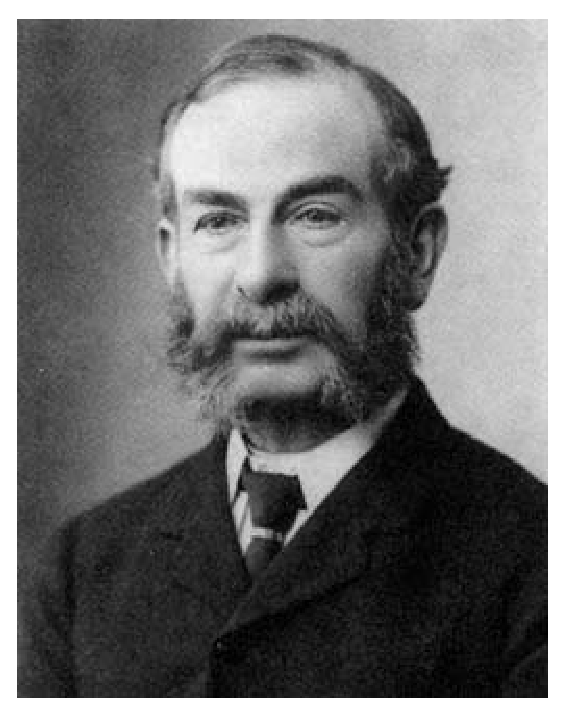
\includegraphics[width=0.9\linewidth]{EdwardRouth.eps} 
    \caption*{\index{Routh, Edward}Edward John Routh (1831-1907), 
             mathématicien anglais.}
\end{marginfigure}
%-------------------------------------------------------------------------------
pour déterminer si ce polynôme possède des racines toutes à partie réelle 
strictement négative. Les polynômes de ce type sont dits en mathématiques 
de Hurwitz\footnote{Un polynôme de Hurwitz est un polynôme à 
coefficients réels dont les racines sont toutes à partie réelle strictement 
négative.}.
C'est pourquoi le critère suivant est également connu sous le nom de 
\textbf{critère de Routh-Hurwitz}.
%-------------------------------------------------------------------------------
\begin{marginfigure}
    \centering
    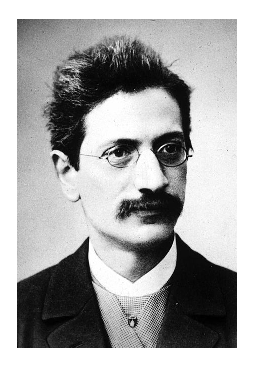
\includegraphics[width=0.9\linewidth]{AdolfHurwitz.eps} 
    \caption*{\index{Hurwitz, Adolf}Adolf Hurwitz (1859-1919),
    mathématicien allemand.}
\end{marginfigure}
%-------------------------------------------------------------------------------
Il est possible de conclure sur la nature des racines d'un polynôme 
en étudiant ses coefficients. Le critère de Routh-Hurwitz se base sur 
cette propriété en posant deux conditions pour établir qu'un polynôme est 
un polynôme de Hurwitz. Dans le cas de l'application de la stabilité des 
systèmes linéaires asservis, la première condition s'énonce 
de la façon suivante :
%-------------------------------------------------------------------------------
\begin{criteria}{Condition nécessaire de Routh-Hurwitz }
    \textbf{Un système asservi d'ordre $n$ est stable en boucle fermée 
    si tous les coefficients ($b_i\forall i\neq n$) de son équation 
    caractéristique sont de même signe que $b_n$.}
\end{criteria}
%-------------------------------------------------------------------------------
\textbf{Cette condition nécessaire s'avère suffisante si le système est du 
premier ou du second ordre.} Pour un ordre supérieur il faut construire le 
tableau de Routh à partir des coefficients de $D(p)$,
pour appliquer une condition supplémentaire. 
%%%%%%%%%%%%%%%%%%%%%%%%%%%%%%%%%%%%%%%%%%%%%%%%%%%%%%%%%%%%%%%%%%%%%%%%%%%%%%%%
%%%%%%%%%%%%%%%%%%%%%%%%%%%%%%%%%%%%%%%%%%%%%%%%%%%%%%%%%%%%%%%%%%%%%%%%%%%%%%%%
\subsection{Tableau de Routh}
%%%%%%%%%%%%%%%%%%%%%%%%%%%%%%%%%%%%%%%%%%%%%%%%%%%%%%%%%%%%%%%%%%%%%%%%%%%%%%%%
%%%%%%%%%%%%%%%%%%%%%%%%%%%%%%%%%%%%%%%%%%%%%%%%%%%%%%%%%%%%%%%%%%%%%%%%%%%%%%%%
Dans le cas où la condition nécessaire est respectée et $n>2$, il faut 
constuire le \textbf{tableau de Routh} à partir des coefficients de l'équation 
caractéristique de la fonction de transfert en boucle fermée.
\newpage
\restoregeometry
\captionsetup{width=0.9\linewidth}
Le tableau de Routh est constitué de $n$ lignes et de $k$ colonnes 
où $k=n/2+1$\footnote{On réalise ici une division entière. Par exemple 
si $n=5$, $k=2+1=3$ et si $n=6$, $k=3+1=4$}. L'élément $A_{ij}$ correspond 
à l'élément de la $i$-ème ligne et $j$-ème colonne.
\[
\begin{matrix}
    p^n    \\
    p^{n-1}\\
    p^{n-2}\\
    p^{n-3}\\
    \vdots \\
    p^1    \\
    p^0    \\
\end{matrix}
\begin{vmatrix}
  A_{11}     & A_{12}     & A_{13}     & \cdots & A_{1(k-1)}     & A_{1k}  \\
  A_{21}     & A_{22}     & A_{23}     & \cdots & A_{2(k-1)}     & A_{2k}  \\
  A_{31}     & A_{32}     & A_{33}     & \cdots & A_{3(k-1)}     & A_{3k}  \\
  A_{41}     & A_{42}     & A_{43}     & \cdots & A_{4(k-1)}     & A_{4k}  \\
  \vdots     & \vdots     & \vdots     & A_{ij} & \vdots         & \vdots  \\
  A_{(n-1)1} & A_{(n-1)2} & A_{(n-1)3} & \cdots & A_{(n-1)(k-1)} & A_{(n-1)k}\\
  A_{n1}     & A_{n2}     & A_{n3}     & \cdots & A_{n(k-1)}     & A_{nk}
\end{vmatrix}
\]

Les deux premières lignes du tableau sont directement construites à partir 
des coefficients de $D(p)$.
\[
    \textbf{paire}\qquad\quad
\begin{matrix}
    p^n    \\
    p^{n-1}\\
    \hline
    \vdots \\
\end{matrix}
\begin{vmatrix}
    b_n       & b_{n-2}    & b_{n-4}    & \cdots & b_2        & b_0  \\
    b_{n-1}   & b_{n-3}    & b_{n-5}    & \cdots & b_1        & 0    \\
    \hline
    \vdots    & \vdots     & \vdots     & \vdots & \vdots     & \vdots  \\
    \end{vmatrix}
\]
si $n$ est impaire la dernière colonne de la seconde ligne est non-nulle:
\[
    \textbf{impaire}\qquad
\begin{matrix}
    p^n    \\
    p^{n-1}\\
    \hline
    \vdots \\
\end{matrix}
\begin{vmatrix}
    b_n       & b_{n-2}    & b_{n-4}    & \cdots & b_3            & b_1    \\
    b_{n-1}   & b_{n-3}    & b_{n-5}    & \cdots & b_2            & b_0    \\
    \hline
    \vdots    & \vdots     & \vdots     & \vdots & \vdots         & \vdots \\
    \end{vmatrix}
\]

Les éléments de la troisième ligne sont construits à partir du 
déterminant\footnote{Le déterminant d'une matrice 2$\times$2 
est tel que $\begin{vmatrix} a & b \\ c & d \end{vmatrix}=ad-bc$} des 
élements des deux premières lignes.
\[
\begin{matrix}
    p^n    \\
    p^{n-1}\\
    \hline
    p^{n-2}\\
    \vdots \\
\end{matrix}
\begin{vmatrix}
    \textcolor{col4}{b_n}       & \textcolor{col4}{b_{n-2}}    & b_{n-4}    
                               & \cdots & b_3            & b_1         \\
    \textcolor{col4}{b_{n-1}}   & \textcolor{col4}{b_{n-3}}    & b_{n-5}    
                               & \cdots & b_2            & b_0         \\
    \hline
    %\hmm{A_{31}}{col4}   & A_{32}     & A_{33} & \cdots & \cdots  & \cdots \\
    A_{31}  & A_{32}     & A_{33}     & \cdots & \cdots         & \cdots   \\
    \vdots    & \vdots     & \vdots     & \vdots & \vdots         & \vdots \\
\end{vmatrix}
\Rightarrow
A_{31}=-\dfrac{1}{b_{n-1}}
\begin{vmatrix} b_{n}  & b_{n-2} \\ b_{n-1} & b_{n-3}
\end{vmatrix}
\]

\[
\begin{matrix}
    p^n    \\
    p^{n-1}\\
    \hline
    p^{n-2}\\
    \vdots \\
\end{matrix}
\begin{vmatrix}
    \textcolor{col1}{b_n}       & b_{n-2}    & \textcolor{col1}{b_{n-4}}    
    & \cdots & b_3        & b_1         \\
    \textcolor{col1}{b_{n-1}}   & b_{n-3}    & \textcolor{col1}{b_{n-5}}    
    & \cdots & b_2            & b_0         \\
    \hline
    %A_{31}    & \hmm{A_{32}}{col1}     & A_{33} & \cdots & \cdots& \cdots  \\
    A_{31}    & A_{32}     & A_{33}     & \cdots & \cdots         & \cdots  \\
    \vdots    & \vdots     & \vdots     & \vdots & \vdots         & \vdots  \\
\end{vmatrix}
\Rightarrow
A_{32}=-\dfrac{1}{b_{n-1}}\begin{vmatrix} b_{n}  & b_{n-4} \\ b_{n-1} & b_{n-5}
\end{vmatrix}
\]

On construit de la même manière la quatrième ligne :
\[
\begin{matrix}
    p^n    \\
    p^{n-1}\\
    \hline
    p^{n-2}\\
    p^{n-3}\\
    \vdots \\
\end{matrix}
\begin{vmatrix}
    b_n       & b_{n-2}    & b_{n-4}    & \cdots & b_3            & b_1 \\
     \textcolor{col4}{b_{n-1}}   & \textcolor{col4}{b_{n-3}}    & b_{n-5}    
                                & \cdots & b_2            & b_0         \\
    \hline
     \textcolor{col4}{A_{31}}    &  \textcolor{col4}{A_{32}}    & A_{33}    
                                & \cdots & \cdots         & \cdots      \\
    A_{41}   & A_{42}     & A_{43}    & \cdots & \cdots   & \cdots      \\
    \vdots   & \vdots     & \vdots    & \vdots & \vdots   & \vdots      \\
    \end{vmatrix}
\Rightarrow
A_{41}=-\dfrac{1}{A_{31}}
\begin{vmatrix} 
A_{21} & A_{22} \\ A_{31} & A_{22}
\end{vmatrix}
\]

\[
\begin{matrix}
    p^n    \\
    p^{n-1}\\
    \hline
    p^{n-2}\\
    p^{n-3}\\
    \vdots \\
\end{matrix}
\begin{vmatrix}
    b_n       & b_{n-2}    & b_{n-4}    & \cdots & b_3            & b_1  \\
    \textcolor{col1}{b_{n-1}}   &  b_{n-3}    & \textcolor{col1}{b_{n-5}}    
    & \cdots & b_2            & b_0         \\
    \hline
    \textcolor{col1}{A_{31}}     &  A_{32}    & \textcolor{col1}{A_{33}}    
    & \cdots & \cdots         & \cdots      \\
    A_{41}      & A_{42}     & A_{43}    & \cdots & \cdots    & \cdots   \\
    \vdots    & \vdots     & \vdots     & \vdots & \vdots     & \vdots   \\
    \end{vmatrix}
    \Rightarrow
    A_{42}=-\dfrac{1}{A_{31}}
    \begin{vmatrix} 
        A_{21} & A_{23} \\ A_{31} & A_{33} 
\end{vmatrix}
\]
Et ainsi de suite jusque la dernière ligne du tableau. 
La formule générale pour obtenir l'élément $A_{ij}$ est alors :
%-------------------------------------------------------------------------------
\begin{bequation}[ams align]
    A_{ij}=-\dfrac{1}{A_{(i-1)1}}
    \begin{vmatrix} 
        A_{(i-2)1} & A_{(i-2)(j+1)} \\ 
        A_{(i-1)1} & A_{(i-1)(j+1)} 
    \end{vmatrix}
\end{bequation}
%-------------------------------------------------------------------------------
Le critère s'applique sur la première colonne ainsi construit dite 
\textbf{colonne des pivots} du tableau de Routh. 
\[
\begin{matrix}
    p^n    \\
    p^{n-1}\\
    p^{n-2}\\
    p^{n-3}\\
    \vdots \\
    p^1    \\
    p^0    \\
\end{matrix}
\begin{vmatrix}
    b_n\DoTikzmark{-1ex}{1.75ex}{n1} & b_{n-2} & b_{n-4}& \cdots & b_2  & b_0\\
    b_{n-1}              & b_{n-3}   & b_{n-5} & \cdots & b_1      & 0 \\
    A_{31}               & A_{32}    & A_{33}  & \cdots & A_{3(k-1)} & 0 \\
    A_{41}               & A_{42}    & A_{43}  & \cdots & 0        & 0 \\
    \vdots               & \vdots    & \vdots  & \vdots & \vdots   & 0 \\
    A_{(n-1)1}           & A_{(n-1)2}& 0       & \cdots & 0        & 0 \\
    b_0\DoTikzmark{-1ex}{-0ex}{n2}    & 0       & 0      & \cdots & 0 & 0
\end{vmatrix}
\]
\colrow[col3,opacity=.2]{n1}{n2}
%-------------------------------------------------------------------------------
\begin{criteria}{Critère de Routh-Hurtwitz}
    \textbf{Un système asservi est stable en boucle fermée
            si tous les termes de la colonne des pivots 
            du tableau de Routh du polynôme caractéristique 
            de la fonction de transfert en boucle fermée sont de même signes.}
\end{criteria}
%-------------------------------------------------------------------------------
%%%%%%%%%%%%%%%%%%%%%%%%%%%%%%%%%%%%%%%%%%%%%%%%%%%%%%%%%%%%%%%%%%%%%%%%%%%%%%%%
\paragraph{Remarques:}
%%%%%%%%%%%%%%%%%%%%%%%%%%%%%%%%%%%%%%%%%%%%%%%%%%%%%%%%%%%%%%%%%%%%%%%%%%%%%%%%
Le nombre de changement de signe, nous donne le nombre de pôles à partie 
réelle positives (instables) de la fonction de transfert en boucle fermée.
%%%%%%%%%%%%%%%%%%%%%%%%%%%%%%%%%%%%%%%%%%%%%%%%%%%%%%%%%%%%%%%%%%%%%%%%%%%%%%%%
\paragraph{Propriétés du tableau de Routh}
%%%%%%%%%%%%%%%%%%%%%%%%%%%%%%%%%%%%%%%%%%%%%%%%%%%%%%%%%%%%%%%%%%%%%%%%%%%%%%%%
Nous énonçons ici quelques propriétés du tableau de Routh 
pour faciliter ou permettre l'application du critère dans 
des cas particuliers~\cite{Ostertag}. 
%-------------------------------------------------------------------------------
\begin{itemize}
    \item Pour simplifier les calculs, il est possible de factorisée par un 
          entier une ligne du tableau.
    \item Dans le cas où le tableau présente un zéro dans la première 
          colonne, il est possible de remplacer par une variable $\epsilon$, 
          et de prendre la limite lorsque $\epsilon\rightarrow 0^+$ ou 
          $\epsilon\rightarrow 0^-$ selon le signe de la colonne des pivots
          qui respecterait le critère.
    \item Une ligne de zéros pour les coefficients de l'avant-dernière ligne 
          du tableau de Routh indique que le polynôme du dénominateur de la 
          fonction de transfert possède une paire de pôles, qui sont racines de 
          l'équation auxiliaire :
    \[
        Ap^2+B=0
    \]
    où $A$ et $B$ sont les coefficients de la ligne précédente du tableau. 
    On peut alors continuer le tableau en remplaçant la ligne de coefficients 
    nuls par les coefficients de la dérivée de l'équation auxiliaire. 
    
    Une ligne de zéro implique la présence d'une paire de racines imaginaires 
    pures donnant lieu à une forme sinuso\"idale dans la réponse transitoire.
    Le système diverge en oscillant s'il y a au moins une racine à partie 
    réelle positive, ou il converge vers des oscillations entretenues si les 
    autres racines ont toutes une partie réelle négative.
\end{itemize}
%-------------------------------------------------------------------------------
%%%%%%%%%%%%%%%%%%%%%%%%%%%%%%%%%%%%%%%%%%%%%%%%%%%%%%%%%%%%%%%%%%%%%%%%%%%%%%%%
%%%%%%%%%%%%%%%%%%%%%%%%%%%%%%%%%%%%%%%%%%%%%%%%%%%%%%%%%%%%%%%%%%%%%%%%%%%%%%%%
\subsection{Exemple d'application du critère de Routh-Hurwitz}
%%%%%%%%%%%%%%%%%%%%%%%%%%%%%%%%%%%%%%%%%%%%%%%%%%%%%%%%%%%%%%%%%%%%%%%%%%%%%%%%
%%%%%%%%%%%%%%%%%%%%%%%%%%%%%%%%%%%%%%%%%%%%%%%%%%%%%%%%%%%%%%%%%%%%%%%%%%%%%%%%

La particularité du critère de Routh-Hurwitz est de permettre d'étudier les 
conditions de stabilité d'un système en fonction des paramètres de la fonction 
de transfert en boucle ouverte.

Dans l'exemple ci-dessous, nous allons considérer un système asservi 
caractérisé par fonction de transfert en boucle ouverte défini par un gain $K$
dont l'on souhaite déterminer la valeur pour assurer la stabilité du système en 
boucle fermée.

Soit un système asservi défini par le schéma-bloc suivant :
%-------------------------------------------------------------------------------
\begin{center}
    \tikzsetnextfilename{routh_exemple-chap_stab-ext}
    \input{tikz/routh_exemple-chap_stab.tex}
\end{center}
%-------------------------------------------------------------------------------
La fonction de transfert en boucle fermée $H_{BF}(p)$ s'écrit :
\[
    H_{BF}(p)=\dfrac{H_{BO}(p)}{1+H_{BO}(p)}=\dfrac{K}{p^3+p^2+3p+K}.
\]
L'équation caractéristique $D(p)$ de $H_{BF}$ est donc 
\[
    D(p)=p^3+p^2+3p+K,
\]
Nous constatons que le système est d'ordre 3 de coefficients :
%-------------------------------------------------------------------------------
\begin{align*}
    b_3&=1\\
    b_2&=1\\
    b_1&=3\\
    b_0&=K
\end{align*}
%-------------------------------------------------------------------------------
Le critère nécessaire de Routh est donc respecté pour $K>0$. L'équation 
caractéristique étant d'ordre 3, il nous faut construire le tableau de Routh, 
afin de vérifier le critère supplémentaire :
\[
\begin{matrix}
    p^3 \\
    p^2 \\
    \hline
    p^1 \\
    p^0 \\
\end{matrix}
\begin{vmatrix}
     1      & 3  \\
     1      & K  \\
    \hline
    A_{31}  & 0  \\
    A_{41}  & 0    
\end{vmatrix}
\]

\[
A_{31}=-\begin{vmatrix}1 & 3 \\ 1 & K\end{vmatrix}=3-K
\]

\[
A_{41}=-\dfrac{1}{A_{31}}\begin{vmatrix} 1 & K \\ A_{31} & 0 \end{vmatrix}=K
\]
\[
\begin{matrix}
    p^3 \\
    p^2 \\
    p^1 \\
    p^0 \\
\end{matrix}
\begin{vmatrix}
    1\DoTikzmark{-0.6ex}{1.75ex}{n3}   & 3  \\
    1\DoTikzmark{-0.6ex}{-6ex}{n4}     & K  \\
    3-K                      & 0  \\
    K                        & 0    
    \end{vmatrix}
\]
\colrow[col3,opacity=.2]{n3}{n4}

La colonne des pivots sont tous de même signe si $3-K>0$ et $K>0$ (déjà établie 
par la condition nécessaire de Routh). La condition sur $K$ pour que le 
système soit stable en boucle fermée est donc :
\[
    0<K<3
\]
%%%%%%%%%%%%%%%%%%%%%%%%%%%%%%%%%%%%%%%%%%%%%%%%%%%%%%%%%%%%%%%%%%%%%%%%%%%%%%%%
%%%%%%%%%%%%%%%%%%%%%%%%%%%%%%%%%%%%%%%%%%%%%%%%%%%%%%%%%%%%%%%%%%%%%%%%%%%%%%%%
%%%%%%%%%%%%%%%%%%%%%%%%%%%%%%%%%%%%%%%%%%%%%%%%%%%%%%%%%%%%%%%%%%%%%%%%%%%%%%%%
\section{Critère graphique du revers
\index{Critère de stabilité! du revers}}
%%%%%%%%%%%%%%%%%%%%%%%%%%%%%%%%%%%%%%%%%%%%%%%%%%%%%%%%%%%%%%%%%%%%%%%%%%%%%%%%
%%%%%%%%%%%%%%%%%%%%%%%%%%%%%%%%%%%%%%%%%%%%%%%%%%%%%%%%%%%%%%%%%%%%%%%%%%%%%%%%
%%%%%%%%%%%%%%%%%%%%%%%%%%%%%%%%%%%%%%%%%%%%%%%%%%%%%%%%%%%%%%%%%%%%%%%%%%%%%%%%
Le critère de Routh s'applique sur la fonction de transfert en boucle fermée. 
Les critères graphiques que nous allons maintenant établir 
permettent d'étudier la stabilité du système en boucle fermée en considérant 
le système en boucle ouverte.

Pour celà considèrons la boucle de contre réaction unitaire 
pour l'asservissement d'un système de fonction de transfert $H(p)$, telle que :
%-------------------------------------------------------------------------------
\begin{center}
    \tikzsetnextfilename{sb_revers-chap_stab-ext}
    \input{tikz/sb_revers-chap_stab.tex}
\end{center}
%-------------------------------------------------------------------------------
la fonction de transfert en boucle ouverte $H_{BO}(p)$ est simplement donné 
par $H(p)$, et comme nous l'avons déjà rencontré à plusieurs occasions, la 
fonction de transfert en boucle fermée $H_{BF}(p)$ est égale à 
\[
    H_{BF}(p)=\dfrac{N(p)}{D(p)}=\dfrac{H_{BO}(p)}{1+H_{BO}(p)},
\]
\'Etudier les pôles de l'équation caractéristique $D(p)=0$ est équivalent 
à étudier l'équation $1+H_{BO}(p)=0$, ou encore 
\[
    D(p)=0\Leftrightarrow1+H_{BO}(p)=0\Leftrightarrow H_{BO}(p)=-1
\]
Il est alors possible d'étudier la fonction de transfert en boucle ouverte par 
rapport à -1 plutôt que par rapport à l'origine. 
%Ce \textbf{point critique}\index{Point critique} du 
%plan complexe $(-1,0)$ de $H_{BO}(p)$.

Pour montrer quelques propriétés de $1+H_{BO}(p)$, nous allons réecrire
ces fonctions de transferts en fonction des polynomes du numérateur et
du dénominateur de la boucle ouverte.
En effet, la fonction de transfert en boucle ouverte
est en générale une fraction rationnelle de la forme:
%-------------------------------------------------------------------------------
\begin{align*}
H_{BO}(p)=\dfrac{N_{BO}(p)}{D_{BO}(p)} \\
1+H_{BO}(p)=\dfrac{N_{BO}(p)+D_{BO}(p)}{D_{BO}(p)}
\end{align*}
%-------------------------------------------------------------------------------
on a alors pour la fonction de transfert en boucle fermée, 
\[
H_{BF}(p)=\dfrac{\dfrac{N_{BO}(p)}{D_{BO}(p)}}{1+\dfrac{N_{BO}(p)}{D_{BO}(p)}}
         =\dfrac{N_{BO}(p)}{D_{BO}(p)+N_{BO}(p)}
\]
Nous remarquons alors que les zéros de $1+H_{BO}(p)$ 
sont les pôles de la fonction de transfert en boucle fermée 
$H_{BF}(p)$ et que les pôles de $1+H_{BO}(p)$ co\"incident avec 
les pôles de $H_{BO}(p)$. Il est donc possible de 
réinterpréter la condition stabilité d'un système asservi :
%-------------------------------------------------------------------------------
\begin{criteria}{Condition de stabilité d'un système asservi (2)}
    \textbf{Un système asservi est stable en boucle fermée si sa fonction 
    de transfert en boucle ouverte ne possède aucun \emph{zéros} à partie 
    réelle positive.}
\end{criteria}
%-------------------------------------------------------------------------------
Nous allons établir un critère que nous pourrons appliquer sur la réponse 
harmonique et ses différentes représentations graphiques.

Supposons le système asservi précédent décrit par la fonction de transfert 
en boucle ouverte $H_{BO}(p)$. Par définition cette fonction de transfert 
est le rapport de la sortie $S(p)$ sur l'écart $\epsilon(p)$ que l'on 
souhaite minimiser.
\[
    S(p)=H_{BO}(p)\epsilon(p)
\]
Considérons une entrée $e(t)$ sinuso\"idale de la forme :
\[
    e(t)=E_0\sin{\omega t}
\]
au premier instant, on a alors 
\[
    \epsilon(t)=E_0\sin{\omega t}
\]
en régime permanent la sortie est alors de la forme (c.f~\cref{chap-repfreq}) :
\[
    s(t)=E_0|H_{BO}(\jw)|\sin{(\omega t+\phi)}
\]
l'écart $\epsilon(t)=e(t)-s(t)$ est maximum pour une sortie en opposition 
de phase. Il existe donc une pulsation $\omega_\pi$ pour laquelle:
%-------------------------------------------------------------------------------
\begin{align*}
    \phi=\arg{H_{BO}(j\omega_\pi)}=-\pi
\end{align*}
%-------------------------------------------------------------------------------
En Pour cette pulsation et ce déphasage: 
\[
    S(p)=-\big|H_{BO}(j\omega_\pi)\big|\epsilon(p)
\]
en posant $K=|H_{BO}(j\omega_\pi)|$, on identifie la \gls{ftbo} a :
\[
    H_{BO}(p)=-K
\]
L'écart dans le domaine de Laplace devient:
%-------------------------------------------------------------------------------
\begin{align*}
    \epsilon(p)&=E(p)-S(p)\\
    \epsilon(p)&=E(p)+K\epsilon(p)
\end{align*}
%-------------------------------------------------------------------------------
Remplaçons à nouveau $\epsilon(p)$ par sa définition (pour simuler une 
deuxième boucle) : 
%-------------------------------------------------------------------------------
\begin{align*}
    \epsilon(p)&=E(p)+K(E(p)-S(p))=E(p)(1+K)+K^2\epsilon(p)
\end{align*}
%-------------------------------------------------------------------------------
et ainsi de suite :
%-------------------------------------------------------------------------------
\begin{align*}
    \epsilon(p)&=E(p)(1+K)+K^2\left(E(p)-S(p)\right)
                =E(p)(1+K+K^2)+K^3\epsilon(p)\\
\end{align*}
%-------------------------------------------------------------------------------
on obtient après $n$ substitutions :
\[
\epsilon(p)=E(p)\sum_{i=0}^{n}K^i+K^n\epsilon(p)
\]
La stabilité du système est alors liée à la convergence de cette somme.
La somme diverge si $K\geq1$ et converge si $K<1$. 
\textbf{Autrement dit le système est stable en boucle fermée 
pour $\big|H_{BO}(\jw)\big|<1$.}

Nous pouvons donc énoncer le critère de stabilité dit du revers :
%-------------------------------------------------------------------------------
\begin{criteria}{Critère de stabilité du revers}
    \textbf{Un système est stable en boucle fermée si lorque le 
    déphasage en boucle ouverte est de -180\degree~le module $|H_{BO}(\jw)|$ 
    est strictement inférieur à 1.}
    Formellement, pour une pulsation $\omega_{\pi}$ telle que 
    $\phi=\arg{\left(H_{BO}(j\omega_\pi)\right)}=-\pi$, 
    le système est stable en boucle fermée si $|H_{BO}(j\omega_\pi)|<1$ ou 
    $20\log{|H_{BO}(j\omega_\pi)|}<\SI{0}{\dB}$.
\end{criteria}
%-------------------------------------------------------------------------------
Dans le plan complexe, un  déphasage de -$\pi$ et un gain naturel de 1 
correspond au point de coordonnées $(-1,0)$ ce que nous avons défini comme 
le point critique à partir de l'équation caractéristique $1+H_{BO}=0$. 
Ce critère revient donc à étudier graphiquement le comportement 
de la réponse harmonique de $H_{BO}(\jw)$ par rapport au point critique.

Nous avons vu que la réponse harmonique peut avoir plusieurs représentations
graphiques (c.f~\Cref{chap-repfreq}). Nous allons maintenant appliquer le 
critère à ces différentes représentations graphiques.

\clearpage
%%%%%%%%%%%%%%%%%%%%%%%%%%%%%%%%%%%%%%%%%%%%%%%%%%%%%%%%%%%%%%%%%%%%%%%%%%%%%%%%
%%%%%%%%%%%%%%%%%%%%%%%%%%%%%%%%%%%%%%%%%%%%%%%%%%%%%%%%%%%%%%%%%%%%%%%%%%%%%%%%
\subsection{Critère du revers dans le plan de Nyquist
\index{Critère de stabilité! du revers! dans le plan de Nyquist}}
%%%%%%%%%%%%%%%%%%%%%%%%%%%%%%%%%%%%%%%%%%%%%%%%%%%%%%%%%%%%%%%%%%%%%%%%%%%%%%%%
%%%%%%%%%%%%%%%%%%%%%%%%%%%%%%%%%%%%%%%%%%%%%%%%%%%%%%%%%%%%%%%%%%%%%%%%%%%%%%%%

Pour énoncer le critère du revers dans le plan de Nyquist. Il nous faut tracer
le lieu de Nyquist de la fonction de transfert en boucle ouverte et observer 
comment il se comporte par rapport au point critique de coordonnées (-1,0) 
dans le plan complexe de $H_{BO}(\jw)$. La~\cref{fig-nyquist_revers} présente 
les lieux de Nyquist de trois systèmes: stable, instable et critique. Observons
que dans le cas stable, le lieu de déphasage $\phi=-\pi$ (c.a.d lorsque le lieu
coupe l'axe des réels négatifs), le module ou le gain naturel $G(\omega)$ (ou 
encore la distance à l'origine) est inférieur à 1. Dans le cas instable ce gain 
est supérieur à 1. Nous appelerons critique le système dont le lieu de Nyquist 
passe par le point critique de coordonnées (-1,0).
%-------------------------------------------------------------------------------
\begin{figure}[!h]
    \centering
    \tikzsetnextfilename{critere_revers_nyquist-chap_stab-ext}
    \input{tikz/critere_revers_nyquist-chap_stab.tex}
    \caption{Représentation schématique de lieux de Nyquist de la fonction 
             de transfert en boucle ouverte de trois systèmes asservis: 
             stable, critique et instable. \label{fig-nyquist_revers}}
\end{figure}
%-------------------------------------------------------------------------------
Nous pouvons maintenant formuler le critère du revers de Nyquist :
%-------------------------------------------------------------------------------
\begin{criteria}{Critère du revers de Nyquist}
\textbf{Un système est stable en boucle fermée si lorsque parcourant 
        le lieu de Nyquist de la boucle ouverte dans le sens des 
        pulsations croissantes, on laisse le point critique sur la 
        \emph{gauche}.}
\end{criteria}
%-------------------------------------------------------------------------------
%\newpage
%%%%%%%%%%%%%%%%%%%%%%%%%%%%%%%%%%%%%%%%%%%%%%%%%%%%%%%%%%%%%%%%%%%%%%%%%%%%%%%%
%%%%%%%%%%%%%%%%%%%%%%%%%%%%%%%%%%%%%%%%%%%%%%%%%%%%%%%%%%%%%%%%%%%%%%%%%%%%%%%%
\subsection{Critère du revers dans le plan de Black
\index{Critère de stabilité! du revers! dans le plan de Black}}
%%%%%%%%%%%%%%%%%%%%%%%%%%%%%%%%%%%%%%%%%%%%%%%%%%%%%%%%%%%%%%%%%%%%%%%%%%%%%%%%
%%%%%%%%%%%%%%%%%%%%%%%%%%%%%%%%%%%%%%%%%%%%%%%%%%%%%%%%%%%%%%%%%%%%%%%%%%%%%%%%
\acpl
%-------------------------------------------------------------------------------
\begin{figure}[!h]
    \centering
    \tikzsetnextfilename{critere_revers_black-chap_stab-ext}
    \begin{tikzpicture}
    \begin{axis}
    [
        height=8cm,
        width=8cm,
        axis lines = center,
        axis line style = thick,
        ticks=none,
        enlargelimits=false,
        xlabel=$\phi$,
        ylabel=$G_{dB}$,
        xlabel style={below right},
        ylabel style={left},
        ymin=-150,
        ymax=60,
        xmin=-270,
        xmax=70
    ]
    \def\da{0.6}
    \def\db{5.0}
    \def\dk{4}
    \def\dpp{1.35}
    \def\colru{col4}
    \addplot[\colru,thick,domain=1e-2:1e-1,samples=100]
    ({-\dpp*atan2(\da*x,(1-\db*x*x))},
     {-\dk*10*log10((1-\db*x*x)*(1-\db*x*x)+\da*\da*x*x)}); 
    \addplot[\colru,thick,domain=1e-1:1e0,samples=100,-{Latex[length=2mm]}] 
    ({-\dpp*atan2(\da*x,(1-\db*x*x))},
     {-\dk*10*log10((1-\db*x*x)*(1-\db*x*x)+\da*\da*x*x)}); 
    \addplot[\colru,thick,domain=0.9e0:1e1,samples=100]  
    ({-\dpp*atan2(\da*x,(1-\db*x*x))},
     {-\dk*10*log10((1-\db*x*x)*(1-\db*x*x)+\da*\da*x*x)});
    \addplot[\colru,thick,domain=1e1:1e2,samples=100]  
    ({-\dpp*atan2(\da*x,(1-\db*x*x))},
     {-\dk*10*log10((1-\db*x*x)*(1-\db*x*x)+\da*\da*x*x)});
    \node [\colru,right]  at (axis cs:  -260, 40.0) {\textbf{instable}};

    \def\da{0.6}
    \def\db{1.0}
    \def\dk{1.5}
    \def\dpp{0.95}
    \edef\colrd{col3}
    \addplot[\colrd,thick,domain=1e-2:1e-1,samples=100]
    ({-\dpp*atan2(\da*x,(1-\db*x*x))},
     {-\dk*10*log10((1-\db*x*x)*(1-\db*x*x)+\da*\da*x*x)}); 
    \addplot[\colrd,thick,domain=1e-1:1e0,samples=100] 
    ({-\dpp*atan2(\da*x,(1-\db*x*x))},
     {-\dk*10*log10((1-\db*x*x)*(1-\db*x*x)+\da*\da*x*x)}); 
    \addplot[\colrd,thick,domain=1e0:1e1,samples=100,-{Latex[length=2mm]}] 
    ({-\dpp*atan2(\da*x,(1-\db*x*x))},
     {-\dk*10*log10((1-\db*x*x)*(1-\db*x*x)+\da*\da*x*x)});
    \addplot[\colrd,thick,domain=0.9e1:1e2,samples=100] 
    ({-\dpp*atan2(\da*x,(1-\db*x*x))},
     {-\dk*10*log10((1-\db*x*x)*(1-\db*x*x)+\da*\da*x*x)});
    \node [\colrd,right]  at (axis cs:  -140, -60.0)   {\textbf{stable}};

    \def\da{0.6}
    \def\db{4.0}
    \def\dk{1.75}
    \def\dpp{1.15}
    \edef\colrt{col1}
    \addplot[\colrt,thick,domain=1e-2:1e-1,samples=100]
    ({-\dpp*atan2(\da*x,(1-\db*x*x))},
     {-\dk*10*log10((1-\db*x*x)*(1-\db*x*x)+\da*\da*x*x)}); 
    \addplot[\colrt,thick,domain=1e-1:1e0,samples=100] 
    ({-\dpp*atan2(\da*x,(1-\db*x*x))},
     {-\dk*10*log10((1-\db*x*x)*(1-\db*x*x)+\da*\da*x*x)}); 
    \addplot[\colrt,thick,domain=1e0:1e1,samples=100,-{Latex[length=2mm]}] 
    ({-\dpp*atan2(\da*x,(1-\db*x*x))},
     {-\dk*10*log10((1-\db*x*x)*(1-\db*x*x)+\da*\da*x*x)});
    \addplot[\colrt,thick,domain=0.9e1:1e2,samples=100] 
    ({-\dpp*atan2(\da*x,(1-\db*x*x))},
     {-\dk*10*log10((1-\db*x*x)*(1-\db*x*x)+\da*\da*x*x)});
    \draw[draw=none,fill=black] (axis cs:-180,0) circle (2pt) node[above] 
    {$(-180,0\mathrm{dB})$};
    \node [\colrt,right]  at (axis cs:  -200, -140.0) {\textbf{critique}};
\end{axis}
\end{tikzpicture}

    \caption{Représentation schématique de lieux de Black de la 
             fonction de transfert en boucle ouverte de trois systèmes 
             asservis: stable, critique et instable.
             \label{fig-black_revers}}
\end{figure}
%-------------------------------------------------------------------------------
%-------------------------------------------------------------------------------
\begin{criteria}{Critère du revers de Black}
\textbf{Un système est stable en boucle fermée si lorsque parcourant 
        le lieu de Black de la boucle ouverte dans le sens des 
        pulsations croissantes, on laisse le point critique sur 
        la \emph{droite}.}
\end{criteria}
%-------------------------------------------------------------------------------
%\newpage
%%%%%%%%%%%%%%%%%%%%%%%%%%%%%%%%%%%%%%%%%%%%%%%%%%%%%%%%%%%%%%%%%%%%%%%%%%%%%%%%
%%%%%%%%%%%%%%%%%%%%%%%%%%%%%%%%%%%%%%%%%%%%%%%%%%%%%%%%%%%%%%%%%%%%%%%%%%%%%%%%
\subsection{Critère du revers dans le plan de Bode
\index{Critère de stabilité! du revers! dans le plan de Bode}}
%%%%%%%%%%%%%%%%%%%%%%%%%%%%%%%%%%%%%%%%%%%%%%%%%%%%%%%%%%%%%%%%%%%%%%%%%%%%%%%%
%%%%%%%%%%%%%%%%%%%%%%%%%%%%%%%%%%%%%%%%%%%%%%%%%%%%%%%%%%%%%%%%%%%%%%%%%%%%%%%%
Il est possible d'appliquer le critère du revers au lieu de transfert de Bode
en boucle ouverte. Le point critique
dans le plan de Bode est représenté par deux verticales coupant les deux 
graphes en gain et en déphasage. De ce fait il faut vérifier deux conditions 
pour respecter le critère du revers dans le plan de Bode 
%-------------------------------------------------------------------------------
\begin{criteria}{Critère du revers de Bode (1)}
\textbf{Un système est stable en boucle fermée si, pour la pulsation 
        $\omega_{1}$ telle que le module de la fonction de transfert en boucle 
        ouverte est égal à 1 (c.a.d $H_{BO}(\omega_{1})=1$ ou $\SI{0}{\dB}$), 
        le déphasage $\phi(\omega_1)$ est supérieur à -180\degree}
\end{criteria}
%-------------------------------------------------------------------------------
%-------------------------------------------------------------------------------
\begin{criteria}{Critère du revers de Bode (2)}
    \textbf{Un système est stable en boucle fermée si, pour la pulsation 
    $\omega_{c}$ (pulsation critique) telle que l'argument de la fonction de 
    transfert en boucle ouverte (déphasage) est égale à -180\degree 
    (c.a.d $\phi(\omega_c)=-180\degree$), le gain $G_{dB}(\omega_c)$ est 
    négatif.}
\end{criteria}
%-------------------------------------------------------------------------------
%-------------------------------------------------------------------------------
\begin{figure}[!h]
\centering
    \tikzsetnextfilename{critere_revers_bode-chap_stab-ext}
    \begin{tikzpicture}
    \begin{axis}
    [
        name=axx,
        ticks=none,
        axis line style = thick,
        xmode=log,
        enlargelimits=false,
        height=4.5cm,
        width=9cm,
        axis x line=center,
        axis y line=left,
        xmin=1e-2,
        xmax=1e2,
        ymin=-60,
        ymax=80,
        xlabel={$\log\omega$},
        xlabel style={below right},
        ylabel={$G_{dB}(\omega)$},
        ylabel style={left,rotate=-90,yshift=3.25em},
        clip=false,
    ]
    \def\dk{9}
    \addplot[signalr,domain=1e-2:1e2]  {\dk+50-20*log10(1+10*x*x)};
    \addplot[signalb,domain=1e-2:1e2]  {\dk+30-20*log10(1+10*x*x)};
    \addplot[signalg,domain=1e-2:1e2]  {\dk+10-20*log10(1+10*x*x)};
    \addplot [col3, mark = *]  coordinates {(3,{\dk+10-20*log10(91)})} {};
    \addplot [col1, mark = *]  coordinates {(3,{\dk+30-20*log10(91)})} {};
    \addplot [col4, mark = *]  coordinates {(3,{\dk+50-20*log10(91)})} {};
    \draw[col3,dashed]  (1e-2,{\dk+10-20*log10(91)}) 
    node[left] {$G(\omega_\pi)$} -- (3,{\dk+10-20*log10(91)});
    \draw[col4,dashed] (1e-2,{\dk+50-20*log10(91)}) 
    node[left] {$G(\omega_\pi)$} -- (3,{\dk+50-20*log10(91)}) ;
    \node (pt1) at (axis cs:3,80) {};
    \draw[]  (1e-2,0)  node[left] {\SI{0}{\dB}} -- (1e2,0);
    \node [col3,right]  at (axis cs: 1e2, -80.0) {\textbf{stable}};
    \node [col1,right]  at (axis cs: 1e2, -60.0) {\textbf{critique}};
    \node [col4,right]  at (axis cs: 1e2, -40.0) {\textbf{instable}};
    \end{axis}
    \begin{axis}
    [
        at={(axx.below south west)},yshift=-0.2cm,anchor=north west,
        ticks=none,
        axis line style = thick,
        xmode=log,
        enlargelimits=false,
        height=4.5cm,
        width=9cm,
        axis x line=center,
        axis y line=left,
        xmin=1e-2,
        xmax=1e2,
        ymin=-270,
        ymax=40,
        xlabel={$\log\omega$},
        xlabel style={below right},
        ylabel={$\hphantom{_DB}\phi(\omega)$},
        ylabel style={left,rotate=-90,yshift=3.25em},
        clip=false,
    ]
    \addplot[very thick,col5,domain=1e-2:1e2, samples=101] {-2.5*atan2(x,1)};
    \def\ttt{0.865}
    \def\ddd{9.1}
    \addplot [col3, mark = *]  coordinates {(\ttt,{-2.5*atan2(\ttt,1)})} {};
    \addplot [col1, mark = *]  coordinates {(3,{-2.5*atan2(3,1)})} {};
    \addplot [col4, mark = *]  coordinates {(\ddd,{-2.5*atan2(\ddd,1)})} {};
    \draw[col3,dashed] (1e-2,{-2.5*atan2(\ttt,1)}) 
    node[left] {$\phi(\omega_{c0})$} -- (\ttt,{-2.5*atan2(\ttt,1)}) ;
    \draw[col4,dashed]  (1e-2,{-2.5*atan2(\ddd,1)}) 
    node[left] {$\phi(\omega_{c0})$} -- (\ddd,{-2.5*atan2(\ddd,1)}) ;
    \draw[black,dashed] (1e-2,-180) node[left] {-180$\degree$} -- (1e2,-180) ;
    \end{axis}
    \draw[col3,dashed] ($(pt1)+(-1,0)$) node[above]{$\omega_{c0}$}--+(0,-7.5cm);
    \draw[col1,dashed] ($(pt1)+(0,0)$)  node[above,text width=1cm,align=center] 
    {$\omega_{c0}$} -- + (0,-7.5cm) ;
    \draw[col4,dashed] ($(pt1)+(0.9,0)$)node[above]{$\omega_{c0}$}--+(0,-7.5cm);
\end{tikzpicture}

    \caption{Représentation schématique de lieux de Bode de la fonction 
             de transfert en boucle ouverte de trois systèmes asservis: 
             stable, critique et instable.}
\end{figure}
%-------------------------------------------------------------------------------
%%%%%%%%%%%%%%%%%%%%%%%%%%%%%%%%%%%%%%%%%%%%%%%%%%%%%%%%%%%%%%%%%%%%%%%%%%%%%%%%
%%%%%%%%%%%%%%%%%%%%%%%%%%%%%%%%%%%%%%%%%%%%%%%%%%%%%%%%%%%%%%%%%%%%%%%%%%%%%%%%
%%%%%%%%%%%%%%%%%%%%%%%%%%%%%%%%%%%%%%%%%%%%%%%%%%%%%%%%%%%%%%%%%%%%%%%%%%%%%%%%
\section{Marge de stabilité et robustesse de la stabilité}
%%%%%%%%%%%%%%%%%%%%%%%%%%%%%%%%%%%%%%%%%%%%%%%%%%%%%%%%%%%%%%%%%%%%%%%%%%%%%%%%
%%%%%%%%%%%%%%%%%%%%%%%%%%%%%%%%%%%%%%%%%%%%%%%%%%%%%%%%%%%%%%%%%%%%%%%%%%%%%%%%
%%%%%%%%%%%%%%%%%%%%%%%%%%%%%%%%%%%%%%%%%%%%%%%%%%%%%%%%%%%%%%%%%%%%%%%%%%%%%%%%
Les critères de stabilité graphiques permettent de s'assurer qu'un système 
est stable ou instable (ou à la limite de la stabilité) en étudiant la réponse
harmonique. Pour estimer la proximité de la réponse harmonique au point 
critique, nous définissons les marges de stabilité. 
%%%%%%%%%%%%%%%%%%%%%%%%%%%%%%%%%%%%%%%%%%%%%%%%%%%%%%%%%%%%%%%%%%%%%%%%%%%%%%%%
%%%%%%%%%%%%%%%%%%%%%%%%%%%%%%%%%%%%%%%%%%%%%%%%%%%%%%%%%%%%%%%%%%%%%%%%%%%%%%%%
%\subsection{Marge de phase}
%%%%%%%%%%%%%%%%%%%%%%%%%%%%%%%%%%%%%%%%%%%%%%%%%%%%%%%%%%%%%%%%%%%%%%%%%%%%%%%%
%%%%%%%%%%%%%%%%%%%%%%%%%%%%%%%%%%%%%%%%%%%%%%%%%%%%%%%%%%%%%%%%%%%%%%%%%%%%%%%%
%-------------------------------------------------------------------------------
\begin{definition}{Marge de phase}
La marge de phase $M_{\phi}$ est définie par :
$M_\phi=\pi+\arg{H_{BO}(j\omega_{c0})}$ où $\omega_{c0}$ est la pulsation de 
coupure pour laquelle le gain naturel $G(\omega_{c0})=|H_{BO}(j\omega_{c0})|=1$
( ou encore 0~\si{\dB} ) 
\end{definition}
%-------------------------------------------------------------------------------
%%%%%%%%%%%%%%%%%%%%%%%%%%%%%%%%%%%%%%%%%%%%%%%%%%%%%%%%%%%%%%%%%%%%%%%%%%%%%%%%
%%%%%%%%%%%%%%%%%%%%%%%%%%%%%%%%%%%%%%%%%%%%%%%%%%%%%%%%%%%%%%%%%%%%%%%%%%%%%%%%
%\subsection{Marge de gain}
%%%%%%%%%%%%%%%%%%%%%%%%%%%%%%%%%%%%%%%%%%%%%%%%%%%%%%%%%%%%%%%%%%%%%%%%%%%%%%%%
%%%%%%%%%%%%%%%%%%%%%%%%%%%%%%%%%%%%%%%%%%%%%%%%%%%%%%%%%%%%%%%%%%%%%%%%%%%%%%%%
%-------------------------------------------------------------------------------
\begin{definition}{Marge de gain}
La marge de gain $M_G$ est définir par $M_G=-20\log{|H(j\omega_\pi)|}$ où 
$\omega_{\pi}$ est la pulsation pour laquelle le déphasage vaut 
\SI{-180}{\degree} $\phi(\omega_\pi)=\arg{(H_{BO}(j\omega_{c0}))}=-\pi$
ou autrement l'argument du point critique dans le plan complexe.
\end{definition}
%-------------------------------------------------------------------------------
Ces marges de stabilités sont en générales imposées par le cahier des charges.
En générales es valeurs pour $M_{\phi}$ de 45 à 60\degree et
pour $M_G$ de 6 à 15~\si{\dB} sont considérées comme satisfaisantes.
%-------------------------------------------------------------------------------
\begin{figure}[!h]
    \centering
    \tikzsetnextfilename{marge_stabilite_nyquist-chap_stab-ext}
    \begin{tikzpicture}
\begin{axis}
    [
    axis lines = center,
    height=0.7\textwidth,
    width=0.7\textwidth,
    ticks=none,
    axis line style = thick,
    %enlargelimits=false,
    xlabel={$\Re{H_{BO}(\jw)}$},
    ylabel={$\Im{H_{BO}(\jw)}$},
    xlabel style={below right},
    ylabel style={right},
    ymin=-1.5,
    ymax=1.5,
    xmin=-1.5,
    xmax=1.5,
%    clip=false
    ]     
    \addplot [black, mark = *] coordinates {( -1, 0)} {};
    \node [above left,xshift=-1ex]  at (axis cs:  -1, 0)   {$(-1,0)$};
    %stable
    \def\xu{-0.206}
    \def\yu{0.4}
    \def\xd{-1}
    \def\yd{0.38}
    \def\xt{-1}
    \def\yt{-4}
    \addplot [-latex,col3,thick,domain=0.85:0.55,samples=50]
    ({(1-x)*((1-x)*(x*\xu)+x*((1-x)*\xu+x*\xd))+
    x*((1-x)*((1-x)*\xu+x*\xd)+x*((1-x)*\xd+x*\xt))},
    {(1-x)*((1-x)*(x*\yu)+x*((1-x)*\yu+x*\yd))+
    x*((1-x)*((1-x)*\yu+x*\yd)+x*((1-x)*\yd+x*\yt))});
    \addplot [-latex,col3,thick,domain=0.56:0.3,samples=50]
    ({(1-x)*((1-x)*(x*\xu)+x*((1-x)*\xu+x*\xd))+
    x*((1-x)*((1-x)*\xu+x*\xd)+x*((1-x)*\xd+x*\xt))},
    {(1-x)*((1-x)*(x*\yu)+x*((1-x)*\yu+x*\yd))+
    x*((1-x)*((1-x)*\yu+x*\yd)+x*((1-x)*\yd+x*\yt))});
    \addplot [col3,thick,domain=0.31:0,samples=50]
    ({(1-x)*((1-x)*(x*\xu)+x*((1-x)*\xu+x*\xd))+
    x*((1-x)*((1-x)*\xu+x*\xd)+x*((1-x)*\xd+x*\xt))},
    {(1-x)*((1-x)*(x*\yu)+x*((1-x)*\yu+x*\yd))+
    x*((1-x)*((1-x)*\yu+x*\yd)+x*((1-x)*\yd+x*\yt))});


    \draw[dashed,thick] (axis cs: 0,0) circle (2.9cm);

    \pgfmathsetmacro{\th}{223}
    \pgfmathsetmacro{\cth}{cos(\th)}
    \pgfmathsetmacro{\sth}{sin(\th)}
    \addplot[col1, mark = *] coordinates {(\cth,\sth)} {};

    \coordinate (o)  at (axis cs: 0.0,0.0);
    \coordinate (p1) at (axis cs: \cth,\sth);
    \coordinate (p2) at (axis cs: -1.0,0.0);
    \coordinate (p3) at (axis cs: -0.47,0);
    \addplot[col3, mark = *] coordinates {(-0.47,0)} {};
    \node [above left,xshift=-1.2ex]  at (p1) {$H_{BO}(j\omega_{c0})$};
    \draw[col1,thick] (axis cs: \cth,\sth) -- (o); 
    \pic[draw,col1,
         dblarw={col1}{2pt}{2pt},
         "$M_\phi$",
         angle radius=0.7cm,
         angle eccentricity=1.5] {angle = p2--o--p1};

    \draw[col1,dashed] (axis cs: -0.47,0) -- (axis cs: -0.47,0.4);
    \draw[dblarw={col1}{2pt}{2pt}] (axis cs: 0,0.4) -- 
    node[midway,above] {$\big|H(j\omega_{\pi})\big|$} (axis cs: -0.47,0.4);
    \node[col1,text width=4cm] at (axis cs: 0.85,1.15) 
    {$M_G=-20\log{\big|H(j\omega_{\pi})\big|}$ 
     $M_\phi=\pi+\phi(H_{BO}(j\omega_{c0}))$};
\end{axis}
\end{tikzpicture}

    \caption{Représentation schématique de lieux de Nyquist de la fonction 
             de transfert en boucle ouverte de trois systèmes asservis: 
             stable, critique et instable. \label{fig-nyquist_revers}}
\end{figure}
%-------------------------------------------------------------------------------
\newpage
\newgeometry{bottom=25mm,outer=60mm,marginparsep=3mm,marginparwidth=50mm}
\captionsetup{width=0.9\linewidth}
%%%%%%%%%%%%%%%%%%%%%%%%%%%%%%%%%%%%%%%%%%%%%%%%%%%%%%%%%%%%%%%%%%%%%%%%%%%%%%%%
%%%%%%%%%%%%%%%%%%%%%%%%%%%%%%%%%%%%%%%%%%%%%%%%%%%%%%%%%%%%%%%%%%%%%%%%%%%%%%%%
%%%%%%%%%%%%%%%%%%%%%%%%%%%%%%%%%%%%%%%%%%%%%%%%%%%%%%%%%%%%%%%%%%%%%%%%%%%%%%%%
\section{Critère de Nyquist\index{Critère de stabilité!de Nyquist}}
%%%%%%%%%%%%%%%%%%%%%%%%%%%%%%%%%%%%%%%%%%%%%%%%%%%%%%%%%%%%%%%%%%%%%%%%%%%%%%%%
%%%%%%%%%%%%%%%%%%%%%%%%%%%%%%%%%%%%%%%%%%%%%%%%%%%%%%%%%%%%%%%%%%%%%%%%%%%%%%%%
%%%%%%%%%%%%%%%%%%%%%%%%%%%%%%%%%%%%%%%%%%%%%%%%%%%%%%%%%%%%%%%%%%%%%%%%%%%%%%%%
Le critère de Nyquist généralise le critère du revers.
Il s'appuie sur le principe de l'argument de Cauchy
\footnote{Nous ne donnerons qu'une présentation élémentaire et sans 
démonstration de ce théorème. Un cours d'analyse complexe permettra de 
compléter cette présentation. On trouvera dans \cite{laas_pc7bis,reg}, 
une introduction plus détaillée ainsi qu'une bibliographie très fournie 
sur le sujet.}.
%-------------------------------------------------------------------------------
\begin{marginfigure}
    \centering
    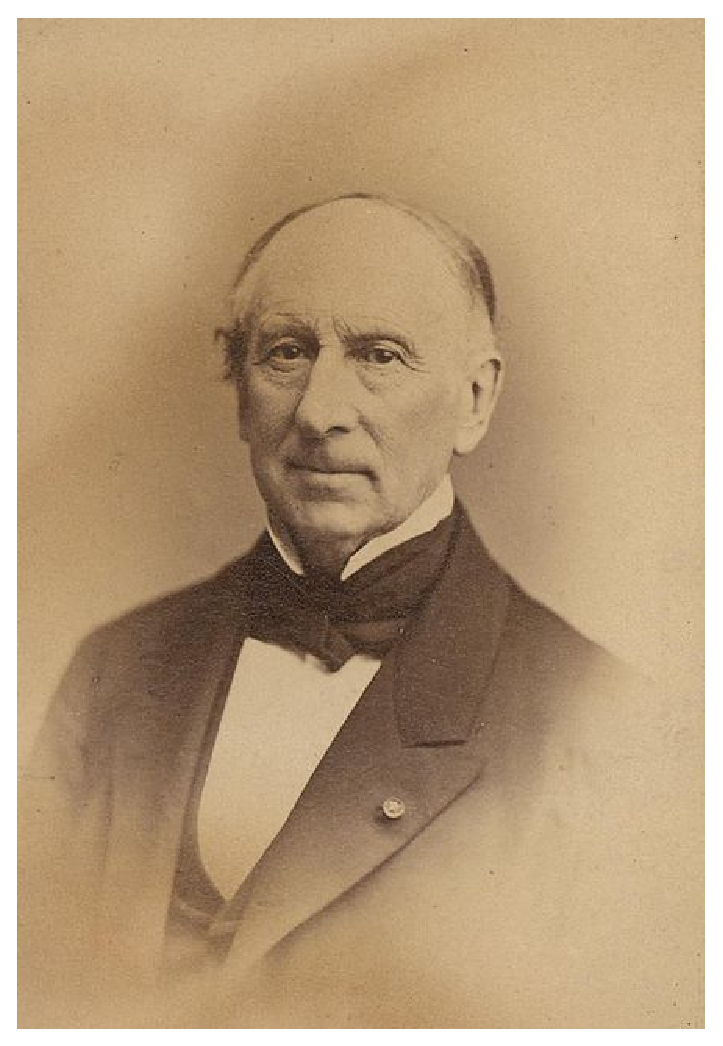
\includegraphics[width=0.9\linewidth]{AugustinCauchy} 
    \caption*{\index{Cauchy, Augustin Louis}\textbf{Augustin Louis Cauchy} 
              (1789-1857), mathématicien français (X1807)}
\end{marginfigure}
%-------------------------------------------------------------------------------
Nous suivrons la présentation \og graphique\fg~ de ce théorème 
et du critère de Nyquist donné par~\cite{reg}. 
%%%%%%%%%%%%%%%%%%%%%%%%%%%%%%%%%%%%%%%%%%%%%%%%%%%%%%%%%%%%%%%%%%%%%%%%%%%%%%%%
\subsection[Image d'un contour d'une fonction de transfert dans $\mathcal{C}$]
{Image d'un contour d'une fonction de transfert dans le plan complexe}
%%%%%%%%%%%%%%%%%%%%%%%%%%%%%%%%%%%%%%%%%%%%%%%%%%%%%%%%%%%%%%%%%%%%%%%%%%%%%%%%
Pour présenter le principe de l'argument de Cauchy, il nous faut déterminer
l'image d'une contour par une fonction de transfert. La~\cref{fig-contour_cauchy} 
présente un exemple de contour  $\mathcal{C}$ parcourant le plan complexe de
la variable $p$ dans le sens des aiguilles d'une montre. On se donne une fonction
de transfert ne possédant aucun pôles et zéros sur $\mathcal{C}$, mais ils
peuvent être contenus dans celui-ci. On appelle $\Gamma$ l'image de 
$\mathcal{C}$ par $F(p)$. \textbf{Le principe de Cauchy nous permet de quantifier le 
nombre de pôles et zéros contenus dans le contour en étudiant l'image de la 
fonction de transfert par ce contour.}
%-------------------------------------------------------------------------------
\begin{figure}[!h]
    \centering
    \tikzsetnextfilename{nyquist_cauchy-chap_stab-ext}
    \begin{tikzpicture}
\begin{axis}
    [
    name=nyy1,
    height=8cm,
    width=8cm,
    axis lines = center,
    ticks=none,
    axis line style = thick,
    enlargelimits=false,
    xlabel=$\Re{p}$,
    ylabel=$\Im{p}$,
    xlabel style={below},
    ylabel style={left},
    ymin=-4,
    ymax=4,
    xmin=-8,
    xmax=8
    ]     
    \pgfmathsetseed{3}
    \draw[
        decoration={markings,mark=at position 0.2 with 
        {\arrow[line width=2pt]{latex}}},
        decoration={markings,mark=at position 0.6 with 
        {\arrow[line width=2pt]{latex}}},
           postaction={decorate},
           thick,
           col4,
           smooth cycle,
           samples=11,
           domain={11:1},
           xshift=3cm,
           yshift=3cm] plot (\x*360/11+5*rnd:1.25cm+0.75cm*rnd) ;
    \node[col4] (ct) at (axis cs:-4,2) {\Large$\mathcal{C}$};
    \addplot[mark=x,ultra thick,only marks,mark size=5pt] 
    coordinates{ (-3.0,-0.5) (-6,-1)};
    \addplot[mark=o,ultra thick,only marks,mark size=5pt] 
    coordinates{ (1,0) (-1,1.2) (-2.1,-1.7) };
\end{axis}
\begin{axis}
    [
    at={(nyy1.south east)},xshift=4ex,
    height=8cm,
    width=8cm,
    axis lines = center,
    ticks=none,
    axis line style = thick,
    enlargelimits=false,
    xlabel=$\Re{F(p)}$,
    ylabel=$\Im{F(p)}$,
    xlabel style={below},
    ylabel style={left},
    ymin=-4,
    ymax=4,
    xmin=-4,
    xmax=4
    ]     
    \def\m{1.0}
    \def\n{2.1}
    \addplot[
    decoration={markings,mark=at position 0.1 with 
    {\arrowreversed[line width=2pt]{latex}}},
    decoration={markings,mark=at position 0.5 with 
    {\arrowreversed[line width=2pt]{latex}}},
    postaction={decorate},
    col1,
    thick,
    domain=1:3,
    samples=50,
    smooth cycle] coordinates 
    {(1.9,-1.5) (0,-2) (-0.75,0.35) (0.25,1.25) (1,0.25) (-0.25,-0.75) 
    (-1.1,-1.25) (-1.5,-1) (-2,0) (-1.5,1.5)  (0,2)  (0.75,1.9) (2,0)}; 
    \node[col1] (ct) at (axis cs:-2.5,2) {\Large$\Gamma:F(\mathcal{C})$};
    \draw[draw=none,fill=black] (axis cs:0,0) circle[radius=2pt];
\end{axis}
\end{tikzpicture}

    \caption{Représentation de la transformation (à gauche) d'un contour $\mathcal{C}$ 
             (à droite) en son image par une fonction analytique $F(p)$. La carte 
             des pôles et zéros est également représentée sur le plan complexe de gauche.
    \label{fig-contour_cauchy}}
\end{figure}
%-------------------------------------------------------------------------------
L'\cref{annexe-cauchy} présente un 

%%%%%%%%%%%%%%%%%%%%%%%%%%%%%%%%%%%%%%%%%%%%%%%%%%%%%%%%%%%%%%%%%%%%%%%%%%%%%%%%
\subsection{Principe de l'argument de Cauchy}
%%%%%%%%%%%%%%%%%%%%%%%%%%%%%%%%%%%%%%%%%%%%%%%%%%%%%%%%%%%%%%%%%%%%%%%%%%%%%%%%
Soit un contour $\mathcal{C}$ parcourant le plan complexe de 
la variable $p$ dans le sens des aiguilles d'une montre et $F(p)$ une fonction 
rationnelle ne possédant ni pôle ni zéro sur $\mathcal{C}$. Le théorème du 
principe de l'argument de Cauchy permet de relier, le nombre de pôles $P$ et 
de zéros $Z$ entourées par le contour $\mathcal{C}$ au comportement de la 
courbe $F(\mathcal{C})$ image $F(p)$ de $\mathcal{C}$.

\begin{theorem}{\'Enoncé du principe de l'argument de Cauchy
    \index{Principe de l'argument de Cauchy}} 
    Si un contour $\mathcal{C}$ contient $Z$ zéros et $P$ pôles d'une fonction 
    analytique $F(p)$ sans en traverser aucun, alors quand on le parcourt dans 
    le sens anti-trigonométrique, le contour $\Gamma=F(\mathcal{C})$ fait un 
    nombre de tours $N$ autour de l'origine dans le sens trigonométrique égal 
    à,
    \[ 
        N=Z-P
    \]
\end{theorem}
On se rapportera à la~\cref{fig-contour_cauchy} pour un exemple d'application 
de ce principe. Dans cet exemple la fonction analytique $F(p)$ possède 2 pôles 
et 3 zéros. Le contour entoure $Z=3$ zéros et $P=1$ pôle.
Le contour $\Gamma=F(\mathcal{C})$ fait alors $N=Z-P=2$ tours autour 
de l'origine dans le sens trigonométrique ($N>0$). Remarquons que les tours 
sont comptés positivement dans le sens trigonométrique (c.f~\cref{fig-ntours}).
%-------------------------------------------------------------------------------
\begin{figure}[!h]
    \centering
    \tikzsetnextfilename{nyquist_ntours_1-chap_stab-ext}
    \input{tikz/nyquist_ntours_1-chap_stab.tex}
    \tikzsetnextfilename{nyquist_ntours_2-chap_stab-ext}
    \input{tikz/nyquist_ntours_2-chap_stab.tex}
    \tikzsetnextfilename{nyquist_ntours_3-chap_stab-ext}
    \begin{tikzpicture}
\begin{axis}[ticks=none,
axis line style = thick,
axis lines = center,
height=4.8cm,
width=4.8cm,
ymin=-1.4,
ymax=1.4,
xmin=-1.4,
xmax=1.4,
clip=false]
\addplot[thick,col4,domain=0:360,samples=100,
decoration={markings,
            mark=at position 0.10 with {\arrowreversed[line width=1pt]{latex}}},
decoration={markings,
            mark=at position 0.20 with {\arrowreversed[line width=1pt]{latex}}},
decoration={markings,
            mark=at position 0.30 with {\arrowreversed[line width=1pt]{latex}}},
decoration={markings,
            mark=at position 0.43 with {\arrowreversed[line width=1pt]{latex}}},
decoration={markings,
            mark=at position 0.50 with {\arrowreversed[line width=1pt]{latex}}},
decoration={markings,
            mark=at position 0.60 with {\arrowreversed[line width=1pt]{latex}}},
decoration={markings,
            mark=at position 0.70 with {\arrowreversed[line width=1pt]{latex}}},
decoration={markings,
            mark=at position 0.80 with {\arrowreversed[line width=1pt]{latex}}},
decoration={markings,
            mark=at position 0.90 with {\arrowreversed[line width=1pt]{latex}}},
postaction={decorate},
] 
({1.0*cos(x)},{1.0*sin(x)});
    \draw[draw=none,fill=black] (axis cs:0.0,0.0) circle[radius=2pt];
\node[below] at (axis cs:0,-1.4) {$N=-1$};
\end{axis}
\end{tikzpicture}


    \tikzsetnextfilename{nyquist_ntours_4-chap_stab-ext}
    \input{tikz/nyquist_ntours_4-chap_stab.tex}
    \tikzsetnextfilename{nyquist_ntours_5-chap_stab-ext}
    \begin{tikzpicture}
\begin{axis}[ticks=none,
axis line style = thick,
axis lines = center,
height=4.8cm,
width=4.8cm,
ymin=-1.4,
ymax=1.4,
xmin=-1.4,
xmax=1.4,
clip=false]
\addplot[thick,col1,domain=0:360,
decoration={markings,mark=at position 0.10 with{\arrow[line width=1pt]{latex}}},
decoration={markings,mark=at position 0.20 with{\arrow[line width=1pt]{latex}}},
decoration={markings,mark=at position 0.30 with{\arrow[line width=1pt]{latex}}},
decoration={markings,mark=at position 0.43 with{\arrow[line width=1pt]{latex}}},
decoration={markings,mark=at position 0.50 with{\arrow[line width=1pt]{latex}}},
decoration={markings,mark=at position 0.60 with{\arrow[line width=1pt]{latex}}},
decoration={markings,mark=at position 0.70 with{\arrow[line width=1pt]{latex}}},
decoration={markings,mark=at position 0.80 with{\arrow[line width=1pt]{latex}}},
decoration={markings,mark=at position 0.90 with{\arrow[line width=1pt]{latex}}},
postaction={decorate},
] coordinates {
({1.0*cos(0)},{1.0*sin(0)})
({0.9994*cos(1)},{0.9994*sin(1)})
({0.9988003599999999*cos(2)},{0.9988003599999999*sin(2)})
({0.9982010797839999*cos(3)},{0.9982010797839999*sin(3)})
({0.9976021591361294*cos(4)},{0.9976021591361294*sin(4)})
({0.9970035978406476*cos(5)},{0.9970035978406476*sin(5)})
({0.9964053956819432*cos(6)},{0.9964053956819432*sin(6)})
({0.995807552444534*cos(7)},{0.995807552444534*sin(7)})
({0.9952100679130672*cos(8)},{0.9952100679130672*sin(8)})
({0.9946129418723193*cos(9)},{0.9946129418723193*sin(9)})
({0.9940161741071959*cos(10)},{0.9940161741071959*sin(10)})
({0.9934197644027315*cos(11)},{0.9934197644027315*sin(11)})
({0.9928237125440899*cos(12)},{0.9928237125440899*sin(12)})
({0.9922280183165634*cos(13)},{0.9922280183165634*sin(13)})
({0.9916326815055734*cos(14)},{0.9916326815055734*sin(14)})
({0.99103770189667*cos(15)},{0.99103770189667*sin(15)})
({0.9904430792755319*cos(16)},{0.9904430792755319*sin(16)})
({0.9898488134279665*cos(17)},{0.9898488134279665*sin(17)})
({0.9892549041399097*cos(18)},{0.9892549041399097*sin(18)})
({0.9886613511974257*cos(19)},{0.9886613511974257*sin(19)})
({0.9880681543867073*cos(20)},{0.9880681543867073*sin(20)})
({0.9874753134940751*cos(21)},{0.9874753134940751*sin(21)})
({0.9868828283059786*cos(22)},{0.9868828283059786*sin(22)})
({0.986290698608995*cos(23)},{0.986290698608995*sin(23)})
({0.9856989241898295*cos(24)},{0.9856989241898295*sin(24)})
({0.9851075048353156*cos(25)},{0.9851075048353156*sin(25)})
({0.9845164403324144*cos(26)},{0.9845164403324144*sin(26)})
({0.9839257304682149*cos(27)},{0.9839257304682149*sin(27)})
({0.9833353750299338*cos(28)},{0.9833353750299338*sin(28)})
({0.9827453738049159*cos(29)},{0.9827453738049159*sin(29)})
({0.9821557265806329*cos(30)},{0.9821557265806329*sin(30)})
({0.9815664331446845*cos(31)},{0.9815664331446845*sin(31)})
({0.9809774932847977*cos(32)},{0.9809774932847977*sin(32)})
({0.9803889067888267*cos(33)},{0.9803889067888267*sin(33)})
({0.9798006734447534*cos(34)},{0.9798006734447534*sin(34)})
({0.9792127930406865*cos(35)},{0.9792127930406865*sin(35)})
({0.978625265364862*cos(36)},{0.978625265364862*sin(36)})
({0.9780380902056431*cos(37)},{0.9780380902056431*sin(37)})
({0.9774512673515197*cos(38)},{0.9774512673515197*sin(38)})
({0.9768647965911087*cos(39)},{0.9768647965911087*sin(39)})
({0.976278677713154*cos(40)},{0.976278677713154*sin(40)})
({0.9756929105065261*cos(41)},{0.9756929105065261*sin(41)})
({0.9751074947602221*cos(42)},{0.9751074947602221*sin(42)})
({0.9745224302633659*cos(43)},{0.9745224302633659*sin(43)})
({0.9739377168052079*cos(44)},{0.9739377168052079*sin(44)})
({0.9733533541751247*cos(45)},{0.9733533541751247*sin(45)})
({0.9727693421626196*cos(46)},{0.9727693421626196*sin(46)})
({0.9721856805573219*cos(47)},{0.9721856805573219*sin(47)})
({0.9716023691489875*cos(48)},{0.9716023691489875*sin(48)})
({0.9710194077274981*cos(49)},{0.9710194077274981*sin(49)})
({0.9704367960828615*cos(50)},{0.9704367960828615*sin(50)})
({0.9698545340052117*cos(51)},{0.9698545340052117*sin(51)})
({0.9692726212848085*cos(52)},{0.9692726212848085*sin(52)})
({0.9686910577120376*cos(53)},{0.9686910577120376*sin(53)})
({0.9681098430774103*cos(54)},{0.9681098430774103*sin(54)})
({0.9675289771715638*cos(55)},{0.9675289771715638*sin(55)})
({0.9669484597852609*cos(56)},{0.9669484597852609*sin(56)})
({0.9663682907093897*cos(57)},{0.9663682907093897*sin(57)})
({0.965788469734964*cos(58)},{0.965788469734964*sin(58)})
({0.965208996653123*cos(59)},{0.965208996653123*sin(59)})
({0.9646298712551311*cos(60)},{0.9646298712551311*sin(60)})
({0.964051093332378*cos(61)},{0.964051093332378*sin(61)})
({0.9634726626763785*cos(62)},{0.9634726626763785*sin(62)})
({0.9628945790787726*cos(63)},{0.9628945790787726*sin(63)})
({0.9623168423313253*cos(64)},{0.9623168423313253*sin(64)})
({0.9617394522259265*cos(65)},{0.9617394522259265*sin(65)})
({0.9611624085545909*cos(66)},{0.9611624085545909*sin(66)})
({0.9605857111094581*cos(67)},{0.9605857111094581*sin(67)})
({0.9600093596827924*cos(68)},{0.9600093596827924*sin(68)})
({0.9594333540669827*cos(69)},{0.9594333540669827*sin(69)})
({0.9588576940545425*cos(70)},{0.9588576940545425*sin(70)})
({0.9582823794381097*cos(71)},{0.9582823794381097*sin(71)})
({0.9577074100104468*cos(72)},{0.9577074100104468*sin(72)})
({0.9571327855644405*cos(73)},{0.9571327855644405*sin(73)})
({0.9565585058931018*cos(74)},{0.9565585058931018*sin(74)})
({0.9559845707895659*cos(75)},{0.9559845707895659*sin(75)})
({0.9554109800470921*cos(76)},{0.9554109800470921*sin(76)})
({0.9548377334590639*cos(77)},{0.9548377334590639*sin(77)})
({0.9542648308189884*cos(78)},{0.9542648308189884*sin(78)})
({0.953692271920497*cos(79)},{0.953692271920497*sin(79)})
({0.9531200565573447*cos(80)},{0.9531200565573447*sin(80)})
({0.9525481845234102*cos(81)},{0.9525481845234102*sin(81)})
({0.9519766556126961*cos(82)},{0.9519766556126961*sin(82)})
({0.9514054696193284*cos(83)},{0.9514054696193284*sin(83)})
({0.9508346263375568*cos(84)},{0.9508346263375568*sin(84)})
({0.9502641255617542*cos(85)},{0.9502641255617542*sin(85)})
({0.9496939670864171*cos(86)},{0.9496939670864171*sin(86)})
({0.9491241507061652*cos(87)},{0.9491241507061652*sin(87)})
({0.9485546762157414*cos(88)},{0.9485546762157414*sin(88)})
({0.947985543410012*cos(89)},{0.947985543410012*sin(89)})
({0.9474167520839659*cos(90)},{0.9474167520839659*sin(90)})
({0.9468483020327155*cos(91)},{0.9468483020327155*sin(91)})
({0.9462801930514959*cos(92)},{0.9462801930514959*sin(92)})
({0.945712424935665*cos(93)},{0.945712424935665*sin(93)})
({0.9451449974807036*cos(94)},{0.9451449974807036*sin(94)})
({0.9445779104822151*cos(95)},{0.9445779104822151*sin(95)})
({0.9440111637359256*cos(96)},{0.9440111637359256*sin(96)})
({0.943444757037684*cos(97)},{0.943444757037684*sin(97)})
({0.9428786901834614*cos(98)},{0.9428786901834614*sin(98)})
({0.9423129629693513*cos(99)},{0.9423129629693513*sin(99)})
({0.9417475751915696*cos(100)},{0.9417475751915696*sin(100)})
({0.9411825266464546*cos(101)},{0.9411825266464546*sin(101)})
({0.9406178171304668*cos(102)},{0.9406178171304668*sin(102)})
({0.9400534464401884*cos(103)},{0.9400534464401884*sin(103)})
({0.9394894143723242*cos(104)},{0.9394894143723242*sin(104)})
({0.9389257207237008*cos(105)},{0.9389257207237008*sin(105)})
({0.9383623652912666*cos(106)},{0.9383623652912666*sin(106)})
({0.9377993478720918*cos(107)},{0.9377993478720918*sin(107)})
({0.9372366682633686*cos(108)},{0.9372366682633686*sin(108)})
({0.9366743262624105*cos(109)},{0.9366743262624105*sin(109)})
({0.936112321666653*cos(110)},{0.936112321666653*sin(110)})
({0.935550654273653*cos(111)},{0.935550654273653*sin(111)})
({0.9349893238810888*cos(112)},{0.9349893238810888*sin(112)})
({0.9344283302867601*cos(113)},{0.9344283302867601*sin(113)})
({0.933867673288588*cos(114)},{0.933867673288588*sin(114)})
({0.9333073526846148*cos(115)},{0.9333073526846148*sin(115)})
({0.9327473682730041*cos(116)},{0.9327473682730041*sin(116)})
({0.9321877198520402*cos(117)},{0.9321877198520402*sin(117)})
({0.931628407220129*cos(118)},{0.931628407220129*sin(118)})
({0.9310694301757968*cos(119)},{0.9310694301757968*sin(119)})
({0.9305107885176913*cos(120)},{0.9305107885176913*sin(120)})
({0.9287428180195076*cos(121)},{0.9287428180195076*sin(121)})
({0.9269782066652705*cos(122)},{0.9269782066652705*sin(122)})
({0.9252169480726065*cos(123)},{0.9252169480726065*sin(123)})
({0.9234590358712685*cos(124)},{0.9234590358712685*sin(124)})
({0.9217044637031131*cos(125)},{0.9217044637031131*sin(125)})
({0.9199532252220771*cos(126)},{0.9199532252220771*sin(126)})
({0.9182053140941552*cos(127)},{0.9182053140941552*sin(127)})
({0.9164607239973763*cos(128)},{0.9164607239973763*sin(128)})
({0.9147194486217813*cos(129)},{0.9147194486217813*sin(129)})
({0.9129814816694*cos(130)},{0.9129814816694*sin(130)})
({0.911246816854228*cos(131)},{0.911246816854228*sin(131)})
({0.909515447902205*cos(132)},{0.909515447902205*sin(132)})
({0.9077873685511908*cos(133)},{0.9077873685511908*sin(133)})
({0.9060625725509436*cos(134)},{0.9060625725509436*sin(134)})
({0.9043410536630968*cos(135)},{0.9043410536630968*sin(135)})
({0.902622805661137*cos(136)},{0.902622805661137*sin(136)})
({0.9009078223303808*cos(137)},{0.9009078223303808*sin(137)})
({0.899196097467953*cos(138)},{0.899196097467953*sin(138)})
({0.8974876248827639*cos(139)},{0.8974876248827639*sin(139)})
({0.8957823983954867*cos(140)},{0.8957823983954867*sin(140)})
({0.8940804118385353*cos(141)},{0.8940804118385353*sin(141)})
({0.892381659056042*cos(142)},{0.892381659056042*sin(142)})
({0.8906861339038356*cos(143)},{0.8906861339038356*sin(143)})
({0.8889938302494182*cos(144)},{0.8889938302494182*sin(144)})
({0.8873047419719443*cos(145)},{0.8873047419719443*sin(145)})
({0.8856188629621976*cos(146)},{0.8856188629621976*sin(146)})
({0.8839361871225694*cos(147)},{0.8839361871225694*sin(147)})
({0.8822567083670365*cos(148)},{0.8822567083670365*sin(148)})
({0.8805804206211392*cos(149)},{0.8805804206211392*sin(149)})
({0.878907317821959*cos(150)},{0.878907317821959*sin(150)})
({0.8772373939180972*cos(151)},{0.8772373939180972*sin(151)})
({0.8755706428696528*cos(152)},{0.8755706428696528*sin(152)})
({0.8739070586482005*cos(153)},{0.8739070586482005*sin(153)})
({0.8722466352367689*cos(154)},{0.8722466352367689*sin(154)})
({0.870589366629819*cos(155)},{0.870589366629819*sin(155)})
({0.8689352468332223*cos(156)},{0.8689352468332223*sin(156)})
({0.8672842698642392*cos(157)},{0.8672842698642392*sin(157)})
({0.8656364297514971*cos(158)},{0.8656364297514971*sin(158)})
({0.8639917205349693*cos(159)},{0.8639917205349693*sin(159)})
({0.8623501362659528*cos(160)},{0.8623501362659528*sin(160)})
({0.8607116710070475*cos(161)},{0.8607116710070475*sin(161)})
({0.8590763188321341*cos(162)},{0.8590763188321341*sin(162)})
({0.857444073826353*cos(163)},{0.857444073826353*sin(163)})
({0.8558149300860829*cos(164)},{0.8558149300860829*sin(164)})
({0.8541888817189193*cos(165)},{0.8541888817189193*sin(165)})
({0.8525659228436533*cos(166)},{0.8525659228436533*sin(166)})
({0.8509460475902504*cos(167)},{0.8509460475902504*sin(167)})
({0.8493292500998288*cos(168)},{0.8493292500998288*sin(168)})
({0.8477155245246392*cos(169)},{0.8477155245246392*sin(169)})
({0.8461048650280424*cos(170)},{0.8461048650280424*sin(170)})
({0.8444972657844891*cos(171)},{0.8444972657844891*sin(171)})
({0.8428927209794986*cos(172)},{0.8428927209794986*sin(172)})
({0.8412912248096376*cos(173)},{0.8412912248096376*sin(173)})
({0.8396927714824992*cos(174)},{0.8396927714824992*sin(174)})
({0.8380973552166825*cos(175)},{0.8380973552166825*sin(175)})
({0.8365049702417708*cos(176)},{0.8365049702417708*sin(176)})
({0.8349156107983114*cos(177)},{0.8349156107983114*sin(177)})
({0.8333292711377946*cos(178)},{0.8333292711377946*sin(178)})
({0.8317459455226328*cos(179)},{0.8317459455226328*sin(179)})
({0.8301656282261398*cos(180)},{0.8301656282261398*sin(180)})
({0.8285883135325102*cos(181)},{0.8285883135325102*sin(181)})
({0.8270139957367983*cos(182)},{0.8270139957367983*sin(182)})
({0.8254426691448984*cos(183)},{0.8254426691448984*sin(183)})
({0.8238743280735231*cos(184)},{0.8238743280735231*sin(184)})
({0.8223089668501834*cos(185)},{0.8223089668501834*sin(185)})
({0.820746579813168*cos(186)},{0.820746579813168*sin(186)})
({0.819187161311523*cos(187)},{0.819187161311523*sin(187)})
({0.8176307057050312*cos(188)},{0.8176307057050312*sin(188)})
({0.8160772073641915*cos(189)},{0.8160772073641915*sin(189)})
({0.8145266606701995*cos(190)},{0.8145266606701995*sin(190)})
({0.8129790600149261*cos(191)},{0.8129790600149261*sin(191)})
({0.8114343998008978*cos(192)},{0.8114343998008978*sin(192)})
({0.8098926744412761*cos(193)},{0.8098926744412761*sin(193)})
({0.8083538783598376*cos(194)},{0.8083538783598376*sin(194)})
({0.8068180059909539*cos(195)},{0.8068180059909539*sin(195)})
({0.8052850517795711*cos(196)},{0.8052850517795711*sin(196)})
({0.8037550101811899*cos(197)},{0.8037550101811899*sin(197)})
({0.8022278756618456*cos(198)},{0.8022278756618456*sin(198)})
({0.8007036426980881*cos(199)},{0.8007036426980881*sin(199)})
({0.7991823057769618*cos(200)},{0.7991823057769618*sin(200)})
({0.7976638593959856*cos(201)},{0.7976638593959856*sin(201)})
({0.7961482980631333*cos(202)},{0.7961482980631333*sin(202)})
({0.7946356162968133*cos(203)},{0.7946356162968133*sin(203)})
({0.7931258086258494*cos(204)},{0.7931258086258494*sin(204)})
({0.7916188695894603*cos(205)},{0.7916188695894603*sin(205)})
({0.7901147937372403*cos(206)},{0.7901147937372403*sin(206)})
({0.7886135756291395*cos(207)},{0.7886135756291395*sin(207)})
({0.7871152098354441*cos(208)},{0.7871152098354441*sin(208)})
({0.7856196909367568*cos(209)},{0.7856196909367568*sin(209)})
({0.784127013523977*cos(210)},{0.784127013523977*sin(210)})
({0.7826371721982814*cos(211)},{0.7826371721982814*sin(211)})
({0.7811501615711047*cos(212)},{0.7811501615711047*sin(212)})
({0.7796659762641196*cos(213)},{0.7796659762641196*sin(213)})
({0.7781846109092178*cos(214)},{0.7781846109092178*sin(214)})
({0.7767060601484902*cos(215)},{0.7767060601484902*sin(215)})
({0.7752303186342081*cos(216)},{0.7752303186342081*sin(216)})
({0.7737573810288031*cos(217)},{0.7737573810288031*sin(217)})
({0.7722872420048483*cos(218)},{0.7722872420048483*sin(218)})
({0.7708198962450391*cos(219)},{0.7708198962450391*sin(219)})
({0.7693553384421735*cos(220)},{0.7693553384421735*sin(220)})
({0.7678935632991334*cos(221)},{0.7678935632991334*sin(221)})
({0.766434565528865*cos(222)},{0.766434565528865*sin(222)})
({0.7649783398543601*cos(223)},{0.7649783398543601*sin(223)})
({0.7635248810086368*cos(224)},{0.7635248810086368*sin(224)})
({0.7620741837347204*cos(225)},{0.7620741837347204*sin(225)})
({0.7606262427856244*cos(226)},{0.7606262427856244*sin(226)})
({0.7591810529243317*cos(227)},{0.7591810529243317*sin(227)})
({0.7577386089237754*cos(228)},{0.7577386089237754*sin(228)})
({0.7562989055668202*cos(229)},{0.7562989055668202*sin(229)})
({0.7548619376462432*cos(230)},{0.7548619376462432*sin(230)})
({0.7534276999647154*cos(231)},{0.7534276999647154*sin(231)})
({0.7519961873347824*cos(232)},{0.7519961873347824*sin(232)})
({0.7505673945788462*cos(233)},{0.7505673945788462*sin(233)})
({0.7491413165291464*cos(234)},{0.7491413165291464*sin(234)})
({0.747717948027741*cos(235)},{0.747717948027741*sin(235)})
({0.7462972839264883*cos(236)},{0.7462972839264883*sin(236)})
({0.744879319087028*cos(237)},{0.744879319087028*sin(237)})
({0.7434640483807626*cos(238)},{0.7434640483807626*sin(238)})
({0.7420514666888391*cos(239)},{0.7420514666888391*sin(239)})
({0.7406415689021303*cos(240)},{0.7406415689021303*sin(240)})
({0.7392343499212163*cos(241)},{0.7392343499212163*sin(241)})
({0.7378298046563659*cos(242)},{0.7378298046563659*sin(242)})
({0.7364279280275189*cos(243)},{0.7364279280275189*sin(243)})
({0.7350287149642666*cos(244)},{0.7350287149642666*sin(244)})
({0.7336321604058345*cos(245)},{0.7336321604058345*sin(245)})
({0.7322382593010633*cos(246)},{0.7322382593010633*sin(246)})
({0.7308470066083913*cos(247)},{0.7308470066083913*sin(247)})
({0.7294583972958354*cos(248)},{0.7294583972958354*sin(248)})
({0.7280724263409732*cos(249)},{0.7280724263409732*sin(249)})
({0.7266890887309254*cos(250)},{0.7266890887309254*sin(250)})
({0.7253083794623366*cos(251)},{0.7253083794623366*sin(251)})
({0.7239302935413582*cos(252)},{0.7239302935413582*sin(252)})
({0.7225548259836296*cos(253)},{0.7225548259836296*sin(253)})
({0.7211819718142607*cos(254)},{0.7211819718142607*sin(254)})
({0.7198117260678136*cos(255)},{0.7198117260678136*sin(255)})
({0.7184440837882847*cos(256)},{0.7184440837882847*sin(256)})
({0.717079040029087*cos(257)},{0.717079040029087*sin(257)})
({0.7157165898530317*cos(258)},{0.7157165898530317*sin(258)})
({0.7143567283323109*cos(259)},{0.7143567283323109*sin(259)})
({0.7129994505484795*cos(260)},{0.7129994505484795*sin(260)})
({0.7116447515924373*cos(261)},{0.7116447515924373*sin(261)})
({0.7102926265644117*cos(262)},{0.7102926265644117*sin(262)})
({0.7089430705739393*cos(263)},{0.7089430705739393*sin(263)})
({0.7075960787398489*cos(264)},{0.7075960787398489*sin(264)})
({0.7062516461902432*cos(265)},{0.7062516461902432*sin(265)})
({0.7049097680624817*cos(266)},{0.7049097680624817*sin(266)})
({0.703570439503163*cos(267)},{0.703570439503163*sin(267)})
({0.702233655668107*cos(268)},{0.702233655668107*sin(268)})
({0.7008994117223376*cos(269)},{0.7008994117223376*sin(269)})
({0.6995677028400652*cos(270)},{0.6995677028400652*sin(270)})
({0.698238524204669*cos(271)},{0.698238524204669*sin(271)})
({0.6969118710086801*cos(272)},{0.6969118710086801*sin(272)})
({0.6955877384537636*cos(273)},{0.6955877384537636*sin(273)})
({0.6942661217507015*cos(274)},{0.6942661217507015*sin(274)})
({0.6929470161193751*cos(275)},{0.6929470161193751*sin(275)})
({0.6916304167887484*cos(276)},{0.6916304167887484*sin(276)})
({0.6903163189968498*cos(277)},{0.6903163189968498*sin(277)})
({0.6890047179907557*cos(278)},{0.6890047179907557*sin(278)})
({0.6876956090265732*cos(279)},{0.6876956090265732*sin(279)})
({0.6863889873694228*cos(280)},{0.6863889873694228*sin(280)})
({0.6850848482934209*cos(281)},{0.6850848482934209*sin(281)})
({0.6837831870816634*cos(282)},{0.6837831870816634*sin(282)})
({0.6824839990262083*cos(283)},{0.6824839990262083*sin(283)})
({0.6811872794280585*cos(284)},{0.6811872794280585*sin(284)})
({0.6798930235971451*cos(285)},{0.6798930235971451*sin(285)})
({0.6786012268523105*cos(286)},{0.6786012268523105*sin(286)})
({0.6773118845212911*cos(287)},{0.6773118845212911*sin(287)})
({0.6760249919407006*cos(288)},{0.6760249919407006*sin(288)})
({0.6747405444560133*cos(289)},{0.6747405444560133*sin(289)})
({0.6734585374215468*cos(290)},{0.6734585374215468*sin(290)})
({0.6721789662004459*cos(291)},{0.6721789662004459*sin(291)})
({0.6709018261646651*cos(292)},{0.6709018261646651*sin(292)})
({0.6696271126949522*cos(293)},{0.6696271126949522*sin(293)})
({0.6683548211808318*cos(294)},{0.6683548211808318*sin(294)})
({0.6670849470205882*cos(295)},{0.6670849470205882*sin(295)})
({0.6658174856212491*cos(296)},{0.6658174856212491*sin(296)})
({0.6645524323985688*cos(297)},{0.6645524323985688*sin(297)})
({0.6632897827770114*cos(298)},{0.6632897827770114*sin(298)})
({0.6620295321897351*cos(299)},{0.6620295321897351*sin(299)})
({0.6607716760785747*cos(300)},{0.6607716760785747*sin(300)})
({0.6595162098940254*cos(301)},{0.6595162098940254*sin(301)})
({0.6582631290952267*cos(302)},{0.6582631290952267*sin(302)})
({0.6570124291499457*cos(303)},{0.6570124291499457*sin(303)})
({0.6557641055345609*cos(304)},{0.6557641055345609*sin(304)})
({0.6545181537340452*cos(305)},{0.6545181537340452*sin(305)})
({0.6532745692419505*cos(306)},{0.6532745692419505*sin(306)})
({0.6520333475603908*cos(307)},{0.6520333475603908*sin(307)})
({0.6507944842000261*cos(308)},{0.6507944842000261*sin(308)})
({0.649557974680046*cos(309)},{0.649557974680046*sin(309)})
({0.6483238145281538*cos(310)},{0.6483238145281538*sin(310)})
({0.6470919992805503*cos(311)},{0.6470919992805503*sin(311)})
({0.6458625244819173*cos(312)},{0.6458625244819173*sin(312)})
({0.6446353856854016*cos(313)},{0.6446353856854016*sin(313)})
({0.6434105784525993*cos(314)},{0.6434105784525993*sin(314)})
({0.6421880983535394*cos(315)},{0.6421880983535394*sin(315)})
({0.6409679409666676*cos(316)},{0.6409679409666676*sin(316)})
({0.639750101878831*cos(317)},{0.639750101878831*sin(317)})
({0.6385345766852611*cos(318)},{0.6385345766852611*sin(318)})
({0.6373213609895592*cos(319)},{0.6373213609895592*sin(319)})
({0.636110450403679*cos(320)},{0.636110450403679*sin(320)})
({0.634901840547912*cos(321)},{0.634901840547912*sin(321)})
({0.633695527050871*cos(322)},{0.633695527050871*sin(322)})
({0.6324915055494743*cos(323)},{0.6324915055494743*sin(323)})
({0.6312897716889303*cos(324)},{0.6312897716889303*sin(324)})
({0.6300903211227213*cos(325)},{0.6300903211227213*sin(325)})
({0.6288931495125881*cos(326)},{0.6288931495125881*sin(326)})
({0.6276982525285142*cos(327)},{0.6276982525285142*sin(327)})
({0.6265056258487101*cos(328)},{0.6265056258487101*sin(328)})
({0.6253152651595975*cos(329)},{0.6253152651595975*sin(329)})
({0.6241271661557942*cos(330)},{0.6241271661557942*sin(330)})
({0.6229413245400982*cos(331)},{0.6229413245400982*sin(331)})
({0.6217577360234721*cos(332)},{0.6217577360234721*sin(332)})
({0.6205763963250275*cos(333)},{0.6205763963250275*sin(333)})
({0.61939730117201*cos(334)},{0.61939730117201*sin(334)})
({0.6182204462997831*cos(335)},{0.6182204462997831*sin(335)})
({0.6170458274518136*cos(336)},{0.6170458274518136*sin(336)})
({0.6158734403796551*cos(337)},{0.6158734403796551*sin(337)})
({0.6147032808429337*cos(338)},{0.6147032808429337*sin(338)})
({0.6135353446093321*cos(339)},{0.6135353446093321*sin(339)})
({0.6123696274545744*cos(340)},{0.6123696274545744*sin(340)})
({0.6112061251624107*cos(341)},{0.6112061251624107*sin(341)})
({0.6100448335246021*cos(342)},{0.6100448335246021*sin(342)})
({0.6088857483409054*cos(343)},{0.6088857483409054*sin(343)})
({0.6077288654190577*cos(344)},{0.6077288654190577*sin(344)})
({0.6065741805747614*cos(345)},{0.6065741805747614*sin(345)})
({0.6054216896316694*cos(346)},{0.6054216896316694*sin(346)})
({0.6042713884213693*cos(347)},{0.6042713884213693*sin(347)})
({0.6031232727833686*cos(348)},{0.6031232727833686*sin(348)})
({0.6019773385650802*cos(349)},{0.6019773385650802*sin(349)})
({0.6008936649799688*cos(-10)},{0.6008936649799688*sin(-10)})
({0.6009537543464668*cos(-9)},{0.6009537543464668*sin(-9)})
({0.6010138497219014*cos(-8)},{0.6010138497219014*sin(-8)})
({0.6010739511068736*cos(-7)},{0.6010739511068736*sin(-7)})
({0.6011340585019842*cos(-6)},{0.6011340585019842*sin(-6)})
({0.6011941719078344*cos(-5)},{0.6011941719078344*sin(-5)})
({0.6012542913250252*cos(-4)},{0.6012542913250252*sin(-4)})
({0.6013144167541576*cos(-3)},{0.6013144167541576*sin(-3)})
({0.601374548195833*cos(-2)},{0.601374548195833*sin(-2)})
({0.6014346856506526*cos(-1)},{0.6014346856506526*sin(-1)})
({0.6014948291192177*cos(0)},{0.6014948291192177*sin(0)})
({0.6015549786021296*cos(1)},{0.6015549786021296*sin(1)})
({0.6016151340999898*cos(2)},{0.6016151340999898*sin(2)})
({0.6016752956133998*cos(3)},{0.6016752956133998*sin(3)})
({0.6017354631429611*cos(4)},{0.6017354631429611*sin(4)})
({0.6017956366892754*cos(5)},{0.6017956366892754*sin(5)})
({0.6018558162529443*cos(6)},{0.6018558162529443*sin(6)})
({0.6019160018345695*cos(7)},{0.6019160018345695*sin(7)})
({0.601976193434753*cos(8)},{0.601976193434753*sin(8)})
({0.6020363910540965*cos(9)},{0.6020363910540965*sin(9)})
({0.6020965946932019*cos(10)},{0.6020965946932019*sin(10)})
({0.6021568043526712*cos(11)},{0.6021568043526712*sin(11)})
({0.6022170200331064*cos(12)},{0.6022170200331064*sin(12)})
({0.6022772417351097*cos(13)},{0.6022772417351097*sin(13)})
({0.6023374694592831*cos(14)},{0.6023374694592831*sin(14)})
({0.6023977032062291*cos(15)},{0.6023977032062291*sin(15)})
({0.6024579429765498*cos(16)},{0.6024579429765498*sin(16)})
({0.6025181887708474*cos(17)},{0.6025181887708474*sin(17)})
({0.6025784405897244*cos(18)},{0.6025784405897244*sin(18)})
({0.6026386984337834*cos(19)},{0.6026386984337834*sin(19)})
({0.6026989623036267*cos(20)},{0.6026989623036267*sin(20)})
({0.602759232199857*cos(21)},{0.602759232199857*sin(21)})
({0.602819508123077*cos(22)},{0.602819508123077*sin(22)})
({0.6028797900738894*cos(23)},{0.6028797900738894*sin(23)})
({0.6029400780528967*cos(24)},{0.6029400780528967*sin(24)})
({0.603000372060702*cos(25)},{0.603000372060702*sin(25)})
({0.603060672097908*cos(26)},{0.603060672097908*sin(26)})
({0.6031209781651178*cos(27)},{0.6031209781651178*sin(27)})
({0.6031812902629343*cos(28)},{0.6031812902629343*sin(28)})
({0.6032416083919606*cos(29)},{0.6032416083919606*sin(29)})
({0.6033019325527998*cos(30)},{0.6033019325527998*sin(30)})
({0.6033622627460551*cos(31)},{0.6033622627460551*sin(31)})
({0.6034225989723296*cos(32)},{0.6034225989723296*sin(32)})
({0.6034829412322269*cos(33)},{0.6034829412322269*sin(33)})
({0.6035432895263502*cos(34)},{0.6035432895263502*sin(34)})
({0.6036036438553029*cos(35)},{0.6036036438553029*sin(35)})
({0.6036640042196884*cos(36)},{0.6036640042196884*sin(36)})
({0.6037243706201103*cos(37)},{0.6037243706201103*sin(37)})
({0.6037847430571723*cos(38)},{0.6037847430571723*sin(38)})
({0.6038451215314781*cos(39)},{0.6038451215314781*sin(39)})
({0.6039055060436312*cos(40)},{0.6039055060436312*sin(40)})
({0.6039658965942356*cos(41)},{0.6039658965942356*sin(41)})
({0.604026293183895*cos(42)},{0.604026293183895*sin(42)})
({0.6040866958132134*cos(43)},{0.6040866958132134*sin(43)})
({0.6041471044827947*cos(44)},{0.6041471044827947*sin(44)})
({0.604207519193243*cos(45)},{0.604207519193243*sin(45)})
({0.6042679399451624*cos(46)},{0.6042679399451624*sin(46)})
({0.6043283667391569*cos(47)},{0.6043283667391569*sin(47)})
({0.6043887995758308*cos(48)},{0.6043887995758308*sin(48)})
({0.6044492384557884*cos(49)},{0.6044492384557884*sin(49)})
({0.604509683379634*cos(50)},{0.604509683379634*sin(50)})
({0.6045701343479719*cos(51)},{0.6045701343479719*sin(51)})
({0.6046305913614067*cos(52)},{0.6046305913614067*sin(52)})
({0.6046910544205428*cos(53)},{0.6046910544205428*sin(53)})
({0.6047515235259848*cos(54)},{0.6047515235259848*sin(54)})
({0.6048119986783375*cos(55)},{0.6048119986783375*sin(55)})
({0.6048724798782052*cos(56)},{0.6048724798782052*sin(56)})
({0.604932967126193*cos(57)},{0.604932967126193*sin(57)})
({0.6049934604229057*cos(58)},{0.6049934604229057*sin(58)})
({0.6050539597689479*cos(59)},{0.6050539597689479*sin(59)})
({0.6051144651649248*cos(60)},{0.6051144651649248*sin(60)})
({0.6051749766114414*cos(61)},{0.6051749766114414*sin(61)})
({0.6052354941091025*cos(62)},{0.6052354941091025*sin(62)})
({0.6052960176585134*cos(63)},{0.6052960176585134*sin(63)})
({0.6053565472602792*cos(64)},{0.6053565472602792*sin(64)})
({0.6054170829150052*cos(65)},{0.6054170829150052*sin(65)})
({0.6054776246232967*cos(66)},{0.6054776246232967*sin(66)})
({0.605538172385759*cos(67)},{0.605538172385759*sin(67)})
({0.6055987262029976*cos(68)},{0.6055987262029976*sin(68)})
({0.6056592860756179*cos(69)},{0.6056592860756179*sin(69)})
({0.6057198520042255*cos(70)},{0.6057198520042255*sin(70)})
({0.6057804239894259*cos(71)},{0.6057804239894259*sin(71)})
({0.6058410020318248*cos(72)},{0.6058410020318248*sin(72)})
({0.6059015861320279*cos(73)},{0.6059015861320279*sin(73)})
({0.6059621762906411*cos(74)},{0.6059621762906411*sin(74)})
({0.6060227725082702*cos(75)},{0.6060227725082702*sin(75)})
({0.606083374785521*cos(76)},{0.606083374785521*sin(76)})
({0.6061439831229996*cos(77)},{0.6061439831229996*sin(77)})
({0.6062045975213118*cos(78)},{0.6062045975213118*sin(78)})
({0.6062652179810639*cos(79)},{0.6062652179810639*sin(79)})
({0.606325844502862*cos(80)},{0.606325844502862*sin(80)})
({0.6063864770873123*cos(81)},{0.6063864770873123*sin(81)})
({0.6064471157350211*cos(82)},{0.6064471157350211*sin(82)})
({0.6065077604465946*cos(83)},{0.6065077604465946*sin(83)})
({0.6065684112226393*cos(84)},{0.6065684112226393*sin(84)})
({0.6066290680637615*cos(85)},{0.6066290680637615*sin(85)})
({0.6066897309705679*cos(86)},{0.6066897309705679*sin(86)})
({0.606750399943665*cos(87)},{0.606750399943665*sin(87)})
({0.6068110749836594*cos(88)},{0.6068110749836594*sin(88)})
({0.6068717560911577*cos(89)},{0.6068717560911577*sin(89)})
({0.6069324432667669*cos(90)},{0.6069324432667669*sin(90)})
({0.6069931365110935*cos(91)},{0.6069931365110935*sin(91)})
({0.6070538358247447*cos(92)},{0.6070538358247447*sin(92)})
({0.6071145412083272*cos(93)},{0.6071145412083272*sin(93)})
({0.607175252662448*cos(94)},{0.607175252662448*sin(94)})
({0.6072359701877142*cos(95)},{0.6072359701877142*sin(95)})
({0.607296693784733*cos(96)},{0.607296693784733*sin(96)})
({0.6073574234541115*cos(97)},{0.6073574234541115*sin(97)})
({0.6074181591964569*cos(98)},{0.6074181591964569*sin(98)})
({0.6074789010123766*cos(99)},{0.6074789010123766*sin(99)})
({0.6075396489024778*cos(100)},{0.6075396489024778*sin(100)})
({0.607600402867368*cos(101)},{0.607600402867368*sin(101)})
({0.6076611629076548*cos(102)},{0.6076611629076548*sin(102)})
({0.6077219290239456*cos(103)},{0.6077219290239456*sin(103)})
({0.607782701216848*cos(104)},{0.607782701216848*sin(104)})
({0.6078434794869696*cos(105)},{0.6078434794869696*sin(105)})
({0.6079042638349182*cos(106)},{0.6079042638349182*sin(106)})
({0.6079650542613018*cos(107)},{0.6079650542613018*sin(107)})
({0.6080258507667279*cos(108)},{0.6080258507667279*sin(108)})
({0.6080866533518046*cos(109)},{0.6080866533518046*sin(109)})
({0.6081474620171398*cos(110)},{0.6081474620171398*sin(110)})
({0.6082082767633414*cos(111)},{0.6082082767633414*sin(111)})
({0.6082690975910178*cos(112)},{0.6082690975910178*sin(112)})
({0.6083299245007768*cos(113)},{0.6083299245007768*sin(113)})
({0.6083907574932269*cos(114)},{0.6083907574932269*sin(114)})
({0.6084515965689762*cos(115)},{0.6084515965689762*sin(115)})
({0.6085124417286331*cos(116)},{0.6085124417286331*sin(116)})
({0.6085732929728059*cos(117)},{0.6085732929728059*sin(117)})
({0.6086341503021032*cos(118)},{0.6086341503021032*sin(118)})
({0.6086950137171334*cos(119)},{0.6086950137171334*sin(119)})
({0.6087558832185052*cos(120)},{0.6087558832185052*sin(120)})
({0.608816758806827*cos(121)},{0.608816758806827*sin(121)})
({0.6088776404827076*cos(122)},{0.6088776404827076*sin(122)})
({0.6089385282467559*cos(123)},{0.6089385282467559*sin(123)})
({0.6089994220995806*cos(124)},{0.6089994220995806*sin(124)})
({0.6090603220417905*cos(125)},{0.6090603220417905*sin(125)})
({0.6091212280739947*cos(126)},{0.6091212280739947*sin(126)})
({0.6091821401968021*cos(127)},{0.6091821401968021*sin(127)})
({0.6092430584108217*cos(128)},{0.6092430584108217*sin(128)})
({0.6093039827166628*cos(129)},{0.6093039827166628*sin(129)})
({0.6093649131149345*cos(130)},{0.6093649131149345*sin(130)})
({0.6094258496062459*cos(131)},{0.6094258496062459*sin(131)})
({0.6094867921912065*cos(132)},{0.6094867921912065*sin(132)})
({0.6095477408704256*cos(133)},{0.6095477408704256*sin(133)})
({0.6096086956445127*cos(134)},{0.6096086956445127*sin(134)})
({0.6096696565140771*cos(135)},{0.6096696565140771*sin(135)})
({0.6097306234797285*cos(136)},{0.6097306234797285*sin(136)})
({0.6097915965420765*cos(137)},{0.6097915965420765*sin(137)})
({0.6098525757017307*cos(138)},{0.6098525757017307*sin(138)})
({0.6099135609593008*cos(139)},{0.6099135609593008*sin(139)})
({0.6099745523153968*cos(140)},{0.6099745523153968*sin(140)})
({0.6100355497706283*cos(141)},{0.6100355497706283*sin(141)})
({0.6100965533256054*cos(142)},{0.6100965533256054*sin(142)})
({0.6101575629809379*cos(143)},{0.6101575629809379*sin(143)})
({0.6102185787372361*cos(144)},{0.6102185787372361*sin(144)})
({0.6102796005951098*cos(145)},{0.6102796005951098*sin(145)})
({0.6103406285551692*cos(146)},{0.6103406285551692*sin(146)})
({0.6104016626180248*cos(147)},{0.6104016626180248*sin(147)})
({0.6104627027842866*cos(148)},{0.6104627027842866*sin(148)})
({0.6105237490545651*cos(149)},{0.6105237490545651*sin(149)})
({0.6105848014294706*cos(150)},{0.6105848014294706*sin(150)})
({0.6106458599096135*cos(151)},{0.6106458599096135*sin(151)})
({0.6107069244956045*cos(152)},{0.6107069244956045*sin(152)})
({0.610767995188054*cos(153)},{0.610767995188054*sin(153)})
({0.6108290719875729*cos(154)},{0.6108290719875729*sin(154)})
({0.6108901548947716*cos(155)},{0.6108901548947716*sin(155)})
({0.6109512439102611*cos(156)},{0.6109512439102611*sin(156)})
({0.6110123390346521*cos(157)},{0.6110123390346521*sin(157)})
({0.6110734402685556*cos(158)},{0.6110734402685556*sin(158)})
({0.6111345476125825*cos(159)},{0.6111345476125825*sin(159)})
({0.6111956610673437*cos(160)},{0.6111956610673437*sin(160)})
({0.6112567806334505*cos(161)},{0.6112567806334505*sin(161)})
({0.6113179063115138*cos(162)},{0.6113179063115138*sin(162)})
({0.611379038102145*cos(163)},{0.611379038102145*sin(163)})
({0.6114401760059552*cos(164)},{0.6114401760059552*sin(164)})
({0.6115013200235558*cos(165)},{0.6115013200235558*sin(165)})
({0.6115624701555582*cos(166)},{0.6115624701555582*sin(166)})
({0.6116236264025737*cos(167)},{0.6116236264025737*sin(167)})
({0.6116847887652139*cos(168)},{0.6116847887652139*sin(168)})
({0.6117459572440904*cos(169)},{0.6117459572440904*sin(169)})
({0.6118071318398148*cos(170)},{0.6118071318398148*sin(170)})
({0.6118683125529988*cos(171)},{0.6118683125529988*sin(171)})
({0.6119294993842541*cos(172)},{0.6119294993842541*sin(172)})
({0.6119906923341926*cos(173)},{0.6119906923341926*sin(173)})
({0.612051891403426*cos(174)},{0.612051891403426*sin(174)})
({0.6121130965925663*cos(175)},{0.6121130965925663*sin(175)})
({0.6121743079022256*cos(176)},{0.6121743079022256*sin(176)})
({0.6122355253330158*cos(177)},{0.6122355253330158*sin(177)})
({0.6122967488855491*cos(178)},{0.6122967488855491*sin(178)})
({0.6123579785604376*cos(179)},{0.6123579785604376*sin(179)})
({0.6124192143582936*cos(180)},{0.6124192143582936*sin(180)})
({0.6140911188134917*cos(181)},{0.6140911188134917*sin(181)})
({0.6157675875678524*cos(182)},{0.6157675875678524*sin(182)})
({0.6174486330819126*cos(183)},{0.6174486330819126*sin(183)})
({0.6191342678502261*cos(184)},{0.6191342678502261*sin(184)})
({0.6208245044014571*cos(185)},{0.6208245044014571*sin(185)})
({0.622519355298473*cos(186)},{0.622519355298473*sin(186)})
({0.6242188331384377*cos(187)},{0.6242188331384377*sin(187)})
({0.6259229505529056*cos(188)},{0.6259229505529056*sin(188)})
({0.6276317202079149*cos(189)},{0.6276317202079149*sin(189)})
({0.6293451548040825*cos(190)},{0.6293451548040825*sin(190)})
({0.6310632670766976*cos(191)},{0.6310632670766976*sin(191)})
({0.6327860697958169*cos(192)},{0.6327860697958169*sin(192)})
({0.6345135757663594*cos(193)},{0.6345135757663594*sin(193)})
({0.6362457978282015*cos(194)},{0.6362457978282015*sin(194)})
({0.6379827488562724*cos(195)},{0.6379827488562724*sin(195)})
({0.6397244417606499*cos(196)},{0.6397244417606499*sin(196)})
({0.6414708894866564*cos(197)},{0.6414708894866564*sin(197)})
({0.6432221050149549*cos(198)},{0.6432221050149549*sin(198)})
({0.6449781013616457*cos(199)},{0.6449781013616457*sin(199)})
({0.646738891578363*cos(200)},{0.646738891578363*sin(200)})
({0.6485044887523718*cos(201)},{0.6485044887523718*sin(201)})
({0.6502749060066657*cos(202)},{0.6502749060066657*sin(202)})
({0.6520501565000638*cos(203)},{0.6520501565000638*sin(203)})
({0.6538302534273089*cos(204)},{0.6538302534273089*sin(204)})
({0.6556152100191655*cos(205)},{0.6556152100191655*sin(205)})
({0.6574050395425177*cos(206)},{0.6574050395425177*sin(206)})
({0.6591997553004687*cos(207)},{0.6591997553004687*sin(207)})
({0.660999370632439*cos(208)},{0.660999370632439*sin(208)})
({0.6628038989142655*cos(209)},{0.6628038989142655*sin(209)})
({0.6646133535583014*cos(210)},{0.6646133535583014*sin(210)})
({0.6664277480135156*cos(211)},{0.6664277480135156*sin(211)})
({0.6682470957655924*cos(212)},{0.6682470957655924*sin(212)})
({0.6700714103370323*cos(213)},{0.6700714103370323*sin(213)})
({0.6719007052872523*cos(214)},{0.6719007052872523*sin(214)})
({0.6737349942126865*cos(215)},{0.6737349942126865*sin(215)})
({0.675574290746887*cos(216)},{0.675574290746887*sin(216)})
({0.677418608560626*cos(217)},{0.677418608560626*sin(217)})
({0.6792679613619964*cos(218)},{0.6792679613619964*sin(218)})
({0.6811223628965146*cos(219)},{0.6811223628965146*sin(219)})
({0.6829818269472221*cos(220)},{0.6829818269472221*sin(220)})
({0.684846367334788*cos(221)},{0.684846367334788*sin(221)})
({0.6867159979176118*cos(222)},{0.6867159979176118*sin(222)})
({0.6885907325919268*cos(223)},{0.6885907325919268*sin(223)})
({0.6904705852919027*cos(224)},{0.6904705852919027*sin(224)})
({0.6923555699897496*cos(225)},{0.6923555699897496*sin(225)})
({0.6942457006958215*cos(226)},{0.6942457006958215*sin(226)})
({0.696140991458721*cos(227)},{0.696140991458721*sin(227)})
({0.6980414563654033*cos(228)},{0.6980414563654033*sin(228)})
({0.6999471095412807*cos(229)},{0.6999471095412807*sin(229)})
({0.7018579651503283*cos(230)},{0.7018579651503283*sin(230)})
({0.7037740373951886*cos(231)},{0.7037740373951886*sin(231)})
({0.7056953405172774*cos(232)},{0.7056953405172774*sin(232)})
({0.7076218887968896*cos(233)},{0.7076218887968896*sin(233)})
({0.709553696553305*cos(234)},{0.709553696553305*sin(234)})
({0.7114907781448955*cos(235)},{0.7114907781448955*sin(235)})
({0.713433147969231*cos(236)},{0.713433147969231*sin(236)})
({0.7153808204631869*cos(237)},{0.7153808204631869*sin(237)})
({0.7173338101030513*cos(238)},{0.7173338101030513*sin(238)})
({0.7192921314046326*cos(239)},{0.7192921314046326*sin(239)})
({0.7212557989233671*cos(240)},{0.7212557989233671*sin(240)})
({0.7232248272544278*cos(241)},{0.7232248272544278*sin(241)})
({0.7251992310328323*cos(242)},{0.7251992310328323*sin(242)})
({0.7271790249335519*cos(243)},{0.7271790249335519*sin(243)})
({0.7291642236716205*cos(244)},{0.7291642236716205*sin(244)})
({0.7311548420022439*cos(245)},{0.7311548420022439*sin(245)})
({0.73315089472091*cos(246)},{0.73315089472091*sin(246)})
({0.735152396663498*cos(247)},{0.735152396663498*sin(247)})
({0.7371593627063893*cos(248)},{0.7371593627063893*sin(248)})
({0.7391718077665776*cos(249)},{0.7391718077665776*sin(249)})
({0.7411897468017803*cos(250)},{0.7411897468017803*sin(250)})
({0.743213194810549*cos(251)},{0.743213194810549*sin(251)})
({0.7452421668323818*cos(252)},{0.7452421668323818*sin(252)})
({0.747276677947834*cos(253)},{0.747276677947834*sin(253)})
({0.7493167432786315*cos(254)},{0.7493167432786315*sin(254)})
({0.751362377987782*cos(255)},{0.751362377987782*sin(255)})
({0.7534135972796886*cos(256)},{0.7534135972796886*sin(256)})
({0.755470416400262*cos(257)},{0.755470416400262*sin(257)})
({0.7575328506370347*cos(258)},{0.7575328506370347*sin(258)})
({0.7596009153192738*cos(259)},{0.7596009153192738*sin(259)})
({0.7616746258180953*cos(260)},{0.7616746258180953*sin(260)})
({0.7637539975465786*cos(261)},{0.7637539975465786*sin(261)})
({0.7658390459598806*cos(262)},{0.7658390459598806*sin(262)})
({0.767929786555351*cos(263)},{0.767929786555351*sin(263)})
({0.7700262348726471*cos(264)},{0.7700262348726471*sin(264)})
({0.7721284064938494*cos(265)},{0.7721284064938494*sin(265)})
({0.7742363170435775*cos(266)},{0.7742363170435775*sin(266)})
({0.7763499821891064*cos(267)},{0.7763499821891064*sin(267)})
({0.7784694176404826*cos(268)},{0.7784694176404826*sin(268)})
({0.7805946391506411*cos(269)},{0.7805946391506411*sin(269)})
({0.7827256625155222*cos(270)},{0.7827256625155222*sin(270)})
({0.7848625035741895*cos(271)},{0.7848625035741895*sin(271)})
({0.787005178208947*cos(272)},{0.787005178208947*sin(272)})
({0.7891537023454573*cos(273)},{0.7891537023454573*sin(273)})
({0.7913080919528603*cos(274)},{0.7913080919528603*sin(274)})
({0.7934683630438916*cos(275)},{0.7934683630438916*sin(275)})
({0.7956345316750013*cos(276)},{0.7956345316750013*sin(276)})
({0.797806613946474*cos(277)},{0.797806613946474*sin(277)})
({0.7999846260025478*cos(278)},{0.7999846260025478*sin(278)})
({0.8021685840315347*cos(279)},{0.8021685840315347*sin(279)})
({0.8043585042659407*cos(280)},{0.8043585042659407*sin(280)})
({0.8065544029825866*cos(281)},{0.8065544029825866*sin(281)})
({0.808756296502729*cos(282)},{0.808756296502729*sin(282)})
({0.8109642011921814*cos(283)},{0.8109642011921814*sin(283)})
({0.813178133461436*cos(284)},{0.813178133461436*sin(284)})
({0.8153981097657856*cos(285)},{0.8153981097657856*sin(285)})
({0.8176241466054461*cos(286)},{0.8176241466054461*sin(286)})
({0.819856260525679*cos(287)},{0.819856260525679*sin(287)})
({0.822094468116914*cos(288)},{0.822094468116914*sin(288)})
({0.8243387860148731*cos(289)},{0.8243387860148731*sin(289)})
({0.8265892309006936*cos(290)},{0.8265892309006936*sin(290)})
({0.8288458195010524*cos(291)},{0.8288458195010524*sin(291)})
({0.8311085685882902*cos(292)},{0.8311085685882902*sin(292)})
({0.8333774949805361*cos(293)},{0.8333774949805361*sin(293)})
({0.8356526155418329*cos(294)},{0.8356526155418329*sin(294)})
({0.837933947182262*cos(295)},{0.837933947182262*sin(295)})
({0.8402215068580695*cos(296)},{0.8402215068580695*sin(296)})
({0.8425153115717919*cos(297)},{0.8425153115717919*sin(297)})
({0.8448153783723829*cos(298)},{0.8448153783723829*sin(298)})
({0.8471217243553394*cos(299)},{0.8471217243553394*sin(299)})
({0.8494343666628293*cos(300)},{0.8494343666628293*sin(300)})
({0.8517533224838187*cos(301)},{0.8517533224838187*sin(301)})
({0.8540786090541995*cos(302)},{0.8540786090541995*sin(302)})
({0.8564102436569174*cos(303)},{0.8564102436569174*sin(303)})
({0.8587482436221007*cos(304)},{0.8587482436221007*sin(304)})
({0.861092626327189*cos(305)},{0.861092626327189*sin(305)})
({0.8634434091970621*cos(306)},{0.8634434091970621*sin(306)})
({0.8658006097041699*cos(307)},{0.8658006097041699*sin(307)})
({0.8681642453686622*cos(308)},{0.8681642453686622*sin(308)})
({0.8705343337585185*cos(309)},{0.8705343337585185*sin(309)})
({0.8729108924896792*cos(310)},{0.8729108924896792*sin(310)})
({0.8752939392261759*cos(311)},{0.8752939392261759*sin(311)})
({0.8776834916802633*cos(312)},{0.8776834916802633*sin(312)})
({0.8800795676125504*cos(313)},{0.8800795676125504*sin(313)})
({0.8824821848321325*cos(314)},{0.8824821848321325*sin(314)})
({0.8848913611967241*cos(315)},{0.8848913611967241*sin(315)})
({0.887307114612791*cos(316)},{0.887307114612791*sin(316)})
({0.8897294630356838*cos(317)},{0.8897294630356838*sin(317)})
({0.8921584244697711*cos(318)},{0.8921584244697711*sin(318)})
({0.8945940169685735*cos(319)},{0.8945940169685735*sin(319)})
({0.8970362586348977*cos(320)},{0.8970362586348977*sin(320)})
({0.8994851676209709*cos(321)},{0.8994851676209709*sin(321)})
({0.901940762128576*cos(322)},{0.901940762128576*sin(322)})
({0.9044030604091869*cos(323)},{0.9044030604091869*sin(323)})
({0.906872080764104*cos(324)},{0.906872080764104*sin(324)})
({0.9093478415445899*cos(325)},{0.9093478415445899*sin(325)})
({0.9118303611520066*cos(326)},{0.9118303611520066*sin(326)})
({0.9143196580379515*cos(327)},{0.9143196580379515*sin(327)})
({0.9168157507043949*cos(328)},{0.9168157507043949*sin(328)})
({0.9193186577038178*cos(329)},{0.9193186577038178*sin(329)})
({0.9218283976393492*cos(330)},{0.9218283976393492*sin(330)})
({0.9243449891649045*cos(331)},{0.9243449891649045*sin(331)})
({0.9268684509853246*cos(332)},{0.9268684509853246*sin(332)})
({0.9293988018565144*cos(333)},{0.9293988018565144*sin(333)})
({0.9319360605855825*cos(334)},{0.9319360605855825*sin(334)})
({0.9344802460309811*cos(335)},{0.9344802460309811*sin(335)})
({0.9370313771026456*cos(336)},{0.9370313771026456*sin(336)})
({0.9395894727621358*cos(337)},{0.9395894727621358*sin(337)})
({0.9421545520227763*cos(338)},{0.9421545520227763*sin(338)})
({0.9447266339497984*cos(339)},{0.9447266339497984*sin(339)})
({0.9473057376604812*cos(340)},{0.9473057376604812*sin(340)})
({0.9498918823242942*cos(341)},{0.9498918823242942*sin(341)})
({0.9524850871630395*cos(342)},{0.9524850871630395*sin(342)})
({0.9550853714509945*cos(343)},{0.9550853714509945*sin(343)})
({0.9576927545150556*cos(344)},{0.9576927545150556*sin(344)})
({0.9603072557348816*cos(345)},{0.9603072557348816*sin(345)})
({0.9629288945430378*cos(346)},{0.9629288945430378*sin(346)})
({0.9655576904251402*cos(347)},{0.9655576904251402*sin(347)})
({0.9681936629200008*cos(348)},{0.9681936629200008*sin(348)})
({0.9708368316197723*cos(349)},{0.9708368316197723*sin(349)})
({0.9734872161700941*cos(350)},{0.9734872161700941*sin(350)})
({0.9761448362702384*cos(351)},{0.9761448362702384*sin(351)})
({0.978809711673256*cos(352)},{0.978809711673256*sin(352)})
({0.9814818621861239*cos(353)},{0.9814818621861239*sin(353)})
({0.9841613076698918*cos(354)},{0.9841613076698918*sin(354)})
({0.9868480680398306*cos(355)},{0.9868480680398306*sin(355)})
({0.9895421632655792*cos(356)},{0.9895421632655792*sin(356)})
({0.9922436133712942*cos(357)},{0.9922436133712942*sin(357)})
({0.9949524384357977*cos(358)},{0.9949524384357977*sin(358)})
({0.9976686585927274*cos(359)},{0.9976686585927274*sin(359)})
({1.0003922940306853*cos(360)},{1.0003922940306853*sin(360)})
};
\draw[draw=none,fill=black] (axis cs:0,0) circle (2pt);
\node[below] at (axis cs:0,-1.4) {$N=2$};
\end{axis}
\end{tikzpicture}

    \tikzsetnextfilename{nyquist_ntours_6-chap_stab-ext}
    \input{tikz/nyquist_ntours_6-chap_stab.tex}
    \caption{Représentation schématique du nombre de tours autour de 
             l'origine de l'image d'une fraction rationnelle d'un contour 
             fermé. Le sens positif est celui du sens trigonométrique.
             \label{fig-ntours}}
\end{figure}
%-------------------------------------------------------------------------------
\clearpage
%%%%%%%%%%%%%%%%%%%%%%%%%%%%%%%%%%%%%%%%%%%%%%%%%%%%%%%%%%%%%%%%%%%%%%%%%%%%%%%%
\subsection{Contours de Nyquist et de Bromwich}
%%%%%%%%%%%%%%%%%%%%%%%%%%%%%%%%%%%%%%%%%%%%%%%%%%%%%%%%%%%%%%%%%%%%%%%%%%%%%%%%
Pour pouvoir appliquer le critère de Nyquist par l'intermédiaire du principe 
de l'argument de Cauchy, il nous faut définir le contour orienté dans le plan 
$p$ qui entoure la zone instable (c.a.d le demi-plan à partie réelle positive).
Nous présentons deux types de contours le contour de Nyquist et ceux de 
Bromwich.
%-------------------------------------------------------------------------------
\begin{marginfigure}
    \centering
    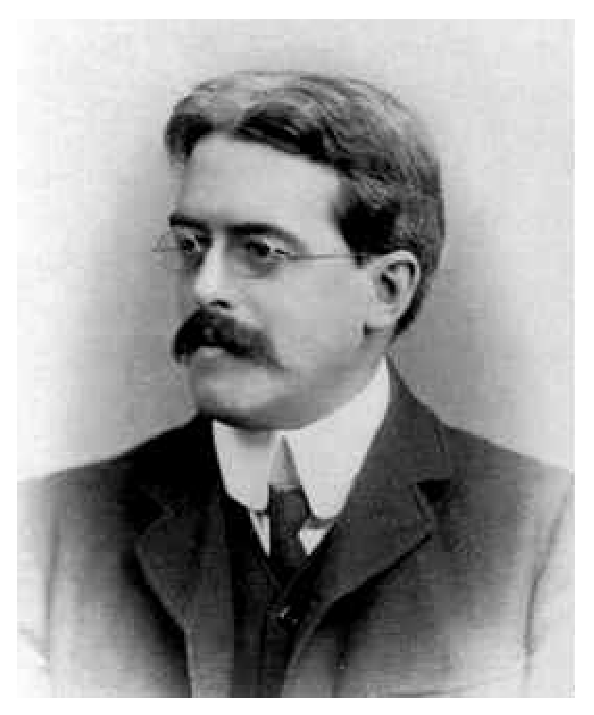
\includegraphics[width=0.9\linewidth]{ThomasBromwich.eps} 
    \caption*{\index{Bromwich, Thomas}\textbf{Thomas John I'Anson Bromwich} 
             (1875-1929), mathématicien anglais.}
\end{marginfigure}
%-------------------------------------------------------------------------------
La~\cref{fig-contours} présente les contours classiques pour l'application 
du critère de Nyquist. Ces contours sont composés de tout l'axe des 
imaginaires, d'un demi cercle de rayon infini centré sur l'origine et dans le
cas où $p=0$ est un pôle ou un zéro de la fonction de transfert en boucle 
ouverte, le contour est également composé d'un cercle de rayon 
$r\rightarrow0$ centré sur les pôles nuls.
%-------------------------------------------------------------------------------
\begin{figure}[!h]
    \centering
    \tikzsetnextfilename{nyquist_contour-chap_stab-ext}
    \begin{tikzpicture}
    \def\rr{1.6}
    \pgfmathsetmacro\ymax{\rr+0.2}
\begin{axis}
    [
    ticks=none,
    axis line style = thick,
    axis lines = center,
    height=6cm,
    width=4cm,
    xlabel=$\Re{p}$,
    ylabel=$\Im{p}$,
    xlabel style={below},
    ylabel style={left,yshift=0.5em},
    ymin=-\ymax,
    ymax=\ymax,
    xmin=-0.8,
    xmax=1.2,
    clip=false]
    \draw[dashed,col1,very thick,-{Latex[length=2.5mm]}] 
    (axis cs:0,-\rr) -- (axis cs:0,-0.8) node[left] {\textbf{III}} ;
    \draw[dashed,col1,very thick,-{Latex[length=2.5mm]}] 
    (axis cs:0,-0.85) -- (axis cs:0,0) ;
    \draw[col1,very thick,-{Latex[length=2.5mm]}] 
    (axis cs:0,0) -- (axis cs:0,0.8) node[left] {\textbf{I}};
    \draw[col1,very thick]                        
    (axis cs:0,0.75) -- (axis cs:0,1.4) ;
    \addplot[col4,very thick,-{Latex[length=2.5mm]},domain=90:60] 
    ({\rr*cos(x)},{\rr*sin(x)});
    \addplot[col4,very thick,domain=62:0] 
    ({\rr*cos(x)},{\rr*sin(x)});
    \addplot[col4,very thick,-{Latex[length=2.5mm]},domain=0:-60] 
    ({\rr*cos(x)},{\rr*sin(x)});
    \addplot[col4,very thick,domain=-58:-90] 
    ({\rr*cos(x)},{\rr*sin(x)});
    \node[right,xshift=0.5em,col4] at 
    (axis cs:{\rr*cos(50)},{\rr*sin(50)}) {\textbf{II}};
    \node[left,col4] at (axis cs:{\rr*cos(90)},{\rr*sin(90)}) 
    {\scriptsize $p\rightarrow+j\infty$};
    \node[left,col4] at (axis cs:{\rr*cos(-90)},{\rr*sin(-90)}) 
    {\scriptsize $p\rightarrow-j\infty$};
    \draw[dashed,thick] (axis cs:0,0) -- 
    (axis cs:{\rr*cos(20)},{\rr*sin(20)}) 
    node[midway,above,yshift=0.5em] {\small$R\rightarrow\infty$};
    \end{axis}
\end{tikzpicture}

    \tikzsetnextfilename{bromwich_contour1-chap_stab-ext}
    \begin{tikzpicture}
    \def\rr{1.6}
    \pgfmathsetmacro\ymax{\rr+0.2}
    \begin{axis}
    [
        ticks=none,
        axis line style = thick,
        axis lines = center,
        height=6cm,
        width=4cm,
        xlabel=$\Re{p}$,
        ylabel=$\Im{p}$,
        xlabel style={below},
        ylabel style={left,yshift=0.5em},
        ymin=-\ymax,
        ymax=\ymax,
        xmin=-0.8,
        xmax=1.2,
        clip=false
    ]
    \draw[dashed,col1,very thick,-{Latex[length=2.5mm]}] 
    (axis cs:0,-1.4) -- (axis cs:0,-0.7) node[left] {\textbf{III}};
    \draw[dashed,col1,very thick] (axis cs:0,-0.75) -- (axis cs:0,-0.15) ;
    \addplot[col3,very thick,domain=-90:-50,samples=10] 
    ({0.15*cos(x)},{0.15*sin(x)});
    \addplot[col3,very thick,domain=-51:-52,samples=10] 
    ({0.15*cos(x)},{0.15*sin(x)});
    \addplot[col3,very thick,domain=-50:60,samples=10] 
    ({0.15*cos(x)},{0.15*sin(x)});
    \addplot[col3,very thick,domain=54:90,samples=10] 
    ({0.15*cos(x)},{0.15*sin(x)});
    \draw[col1,thick,-{Latex[length=2.5mm]}]  
    (axis cs:0,0.15) -- (axis cs:0,0.7) node[left] {\textbf{I}} ;
    \draw[col1,thick]        (axis cs:0,0.65) -- (axis cs:0,\rr) ;
    \addplot[col4,very thick,-{Latex[length=2.5mm]},domain=90:60,samples=50] 
    ({\rr*cos(x)},{\rr*sin(x)});
    \addplot[col4,very thick,-{Latex[length=2.5mm]},domain=62:-60,samples=50] 
    ({\rr*cos(x)},{\rr*sin(x)});
    \addplot[col4,very thick,domain=-58:-90,samples=10] 
    ({\rr*cos(x)},{\rr*sin(x)});
    \node[right,xshift=0.5em,col4] at 
    (axis cs:{\rr*cos(50)},{\rr*sin(50)}) {\textbf{II}};
    \node[right,col3] at 
    (axis cs:{0.20*cos(60)},{0.20*sin(60)}) {\textbf{IV}};
    \node[left,col3] at (axis cs:{-0.15*cos(90)},{0.15*sin(90)}) 
    {\scriptsize $p\rightarrow0^+$};
    \node[left,col3] at (axis cs:{-0.15*cos(-90)},{0.15*sin(-90)}) 
    {\scriptsize $p\rightarrow0^-$};
    \node[left,col4] at (axis cs:{\rr*cos(90)},{\rr*sin(90)}) 
    {\scriptsize $p\rightarrow+j\infty$};
    \node[left,col4] at (axis cs:{\rr*cos(-90)},{\rr*sin(-90)}) 
    {\scriptsize $p\rightarrow-j\infty$};
\end{axis}
\end{tikzpicture}

    \tikzsetnextfilename{bromwich_contour2-chap_stab-ext}
    \begin{tikzpicture}
    \def\rr{1.6}
    \pgfmathsetmacro\ymax{\rr+0.2}
    \begin{axis}[
        ticks=none,
        axis line style = thick,
        axis lines = center,
        height=6cm,
        width=4cm,
        xlabel=$\Re{p}$,
        ylabel=$\Im{p}$,
        xlabel style={below},
        ylabel style={left,yshift=0.5em},
        ymin=-\ymax,
        ymax=\ymax,
        xmin=-0.8,
        xmax=1.2,
        clip=false
    ]
    \draw[col5,thick,-{Latex[length=2.5mm]}] 
    (axis cs:0,-1.4) -- (axis cs:0,-1.0);
    \draw[col5,thick] (axis cs:0,-1.1) -- (axis cs:0,-0.85) ;
    \addplot[col5,very thick,domain=-90:-50,samples=10] 
    ({0.15*cos(x)},{-0.7+0.15*sin(x)});
    \addplot[col5,very thick,domain=-51:-52,samples=10] 
    ({0.15*cos(x)},{-0.7+0.15*sin(x)});
    \addplot[col5,very thick,domain=-50:60,samples=10]  
    ({0.15*cos(x)},{-0.7+0.15*sin(x)});
    \addplot[col5,very thick,domain=54:90,samples=10] 
    ({0.15*cos(x)},{-0.7+0.15*sin(x)});
    \draw[col5,thick,-{Latex[length=2.5mm]}] 
    (axis cs:0,-0.55) -- (axis cs:0,-0.3) ;
    \draw[col5,thick] (axis cs:0,-0.35) -- (axis cs:0,-0.15) ;
    \addplot[col5,very thick,domain=-90:-50,samples=10] 
    ({0.15*cos(x)},{0.15*sin(x)});
    \addplot[col5,very thick,domain=-51:-52,samples=10] 
    ({0.15*cos(x)},{0.15*sin(x)});
    \addplot[col5,very thick,domain=-50:60,samples=10]  
    ({0.15*cos(x)},{0.15*sin(x)});
    \addplot[col5,very thick,domain=54:90,samples=10]   
    ({0.15*cos(x)},{0.15*sin(x)});
    \draw[col5,thick,-{Latex[length=2.5mm]}]    
    (axis cs:0,0.15) -- (axis cs:0,0.4) ;
    \draw[col5,thick]        
    (axis cs:0,0.35) -- (axis cs:0,0.55) ;
    \addplot[col5,very thick,domain=-90:-50,samples=10] 
    ({0.15*cos(x)},{0.7+0.15*sin(x)});
    \addplot[col5,very thick,domain=-51:-52,samples=10] 
    ({0.15*cos(x)},{0.7+0.15*sin(x)});
    \addplot[col5,very thick,domain=-50:60,samples=10]  
    ({0.15*cos(x)},{0.7+0.15*sin(x)});
    \addplot[col5,very thick,domain=54:90,samples=10]   
    ({0.15*cos(x)},{0.7+0.15*sin(x)});
    \draw[col5,thick,-{Latex[length=2.5mm]}]    
    (axis cs:0,0.85) -- (axis cs:0,1.1) ;
    \draw[col5,thick]        (axis cs:0,1.0) -- (axis cs:0,\rr) ;
    \addplot[col5,very thick,-{Latex[length=2.5mm]},domain=90:60,samples=50] 
    ({\rr*cos(x)},{\rr*sin(x)});
    \addplot[col5,very thick,-{Latex[length=2.5mm]},domain=62:-60,samples=50] 
    ({\rr*cos(x)},{\rr*sin(x)});
    \addplot[col5,very thick,domain=-58:-90,samples=10] 
    ({\rr*cos(x)},{\rr*sin(x)});
    \draw[dashed,thick] (axis cs:0,0) -- (axis cs:{\rr*cos(20)},{\rr*sin(20)})
    node[midway,above,yshift=0.5em] {\small$R\rightarrow\infty$};
    \addplot[mark=x,black,ultra thick,only marks,mark size=4pt] 
    coordinates {(0,0) (0,-0.7) (0,0.7)};
    \node[left] at (axis cs:0,0.7) {$p_1$};
    \node[left] at (axis cs:0,-0.7) {$p_2$};
%    \node[below, text width=6cm,text justified,align=center] at 
%    (axis cs:0,-1.6) 
%    {(c) 0, $p_1$ et $p_2$ sont des pôles\\ ou zéros de $H_{BO}$};
    %\draw[green,ultra thick] (axis cs:0,0) circle[radius=1.9cm];
    \end{axis}
\end{tikzpicture}

    \caption{(a) Contour de Nyquist :  $H_{BO}$ ne possède aucun pôle ou zéro 
             et contours de Bromwich: (b) 0 est un pôle\\ ou zéro de $H_{BO}$
             (c) 0, $p_1$ et $p_2$ sont des pôles\\ ou zéros de $H_{BO}$.
             \label{fig-contours}} 
\end{figure}
%-------------------------------------------------------------------------------
%%%%%%%%%%%%%%%%%%%%%%%%%%%%%%%%%%%%%%%%%%%%%%%%%%%%%%%%%%%%%%%%%%%%%%%%%%%%%%%%
\paragraph{Contour de Nyquist}
%%%%%%%%%%%%%%%%%%%%%%%%%%%%%%%%%%%%%%%%%%%%%%%%%%%%%%%%%%%%%%%%%%%%%%%%%%%%%%%%
La~\cref{fig-contours} (a) présente le contour de Nyquist. Celui-ci est 
composé de 3 portions:
%-------------------------------------------------------------------------------
\begin{itemize}
    \item \textbf{I} : l'axe des imaginaires positifs pour laquelle $p=\jw$ 
          avec $\omega\in[0,\infty[$,
    \item \textbf{II}: un demi-cercle de rayon $R$ entourant tout le 
          demi-plan complexe de partie réelle positive et pour lequel 
          $p=Re^{j\theta}$ avec $R\rightarrow\infty$ et $\theta\in[0,\pi/2]$,
    \item \textbf{III}: l'axe des imaginaires négatifs  pour laquelle $p=-\jw$ 
          avec $\omega\in]-\infty,0]$, symétrique de \textbf{I}
\end{itemize}
%-------------------------------------------------------------------------------
%La courbe image d'une fonction de transfert $H_{BO}(p)$
%en boucle ouverte de ces deux portions. 
L'image de la portion \textbf{I} est donné par 
$H_{BO}(\boldsymbol{\mathrm{I}})=H_{BO}(\jw)$, ce qui correspond au lieu de 
Nyquist pour $\omega\in[0,\infty[$. L'image de la portion \textbf{II} est 
l'origine du plan en 0. L'image de la portion \textbf{III} peut être 
déterminé à partir de l'image de la portion \textbf{I} par symétrie par 
rapport à l'axe des réels\footnote{On notera en effet que 
$H_{BO}(-\jw)=\Re{H_{BO}(\jw)}-\Im{H_{BO}(\jw)}$}.
%%%%%%%%%%%%%%%%%%%%%%%%%%%%%%%%%%%%%%%%%%%%%%%%%%%%%%%%%%%%%%%%%%%%%%%%%%%%%%%%
\paragraph{Exemple}
%%%%%%%%%%%%%%%%%%%%%%%%%%%%%%%%%%%%%%%%%%%%%%%%%%%%%%%%%%%%%%%%%%%%%%%%%%%%%%%%
Déterminons l'image par le contour de Bromwich de la fonction de transfert 
suivante : $H_1(p)=\dfrac{1}{1+p}$
%-------------------------------------------------------------------------------
\begin{figure}[!h]
    \centering
    \tikzsetnextfilename{nyquist_contours_exemple_1-chap_stab-ext}
    \begin{tikzpicture}
\begin{axis}
    [
    name=aaa1,
    ticks=none,
    axis line style = thick,
    axis lines = center,
    height=6cm,
    width=6cm,
    xlabel=$\Re{p}$,
    ylabel=$\Im{p}$,
    xlabel style={below},
    ylabel style={left,yshift=0.5em},
    ymin=-1.6,
    ymax=1.6,
    xmin=-0.8,
    xmax=2.4,
    clip=false]
    \draw[dashed,col1,very thick,-{Latex[length=2.5mm]}] 
    (axis cs:0,-1.4) -- (axis cs:0,-0.8) node[left] {\textbf{III}} ;
    \draw[dashed,col1,very thick,-{Latex[length=2.5mm]}] 
    (axis cs:0,-0.85) -- (axis cs:0,0) ;
    \draw[col1,very thick,-{Latex[length=2.5mm]}] 
    (axis cs:0,0) -- (axis cs:0,0.8) node[left] {\textbf{I}};
    \draw[col1,very thick]                        
    (axis cs:0,0.75) -- (axis cs:0,1.4) ;
    \addplot[col4,very thick,-{Latex[length=2.5mm]},domain=90:60] 
    ({1.4*cos(x)},{1.4*sin(x)});
    \addplot[col4,very thick,domain=62:0] 
    ({1.4*cos(x)},{1.4*sin(x)});
    \addplot[col4,very thick,-{Latex[length=2.5mm]},domain=0:-60] 
    ({1.4*cos(x)},{1.4*sin(x)});
    \addplot[col4,very thick,domain=-58:-90] 
    ({1.4*cos(x)},{1.4*sin(x)});
    \node[right,xshift=0.5em,col4] at 
    (axis cs:{1.4*cos(50)},{1.4*sin(50)}) {\textbf{II}};
    \node[left,col4] at (axis cs:{1.4*cos(90)},{1.4*sin(90)}) 
    {\scriptsize $p\rightarrow+j\infty$};
    \node[left,col4] at (axis cs:{1.4*cos(-90)},{1.4*sin(-90)}) 
    {\scriptsize $p\rightarrow-j\infty$};
    \end{axis}
    \draw[dblarw={black}{3pt}{3pt}] (5.2,2.18) -- 
    node[midway,above]  {$H_1(p)$} (7.0,2.18) ;
\begin{axis}[
    name=aaa2,
    at={(aaa1.south east)},xshift=15ex,
    ticks=none,
    axis line style = thick,
    axis lines = center,
    height=6cm,
    width=6cm,
    xlabel=$\Re{H_1(p)}$,
    ylabel=$\Im{H_1(p)}$,
    xlabel style={below right},
    ylabel style={left,yshift=0.5em},
    ymin=-0.6,
    ymax=0.6,
    xmin=-0.2,
    xmax=1.1,
    clip=false]
    \def\ttt{1.0}
    \addplot[col1,very thick,-{Latex[length=2.5mm]},domain=0:0.9,samples=201] 
    ({1/(1+\ttt*x*x)},{-x/(1+\ttt*x*x)});
    \addplot[col1,very thick,domain=0.89:10,samples=201] 
    ({1/(1+\ttt*x*x)},{-x/(1+\ttt*x*x)});
    \addplot[col1,very thick,domain=10:20,samples=201] 
    ({1/(1+\ttt*x*x)},{-x/(1+\ttt*x*x)});
    \addplot[dashed,col1,very thick,domain=0:0.9,samples=201] 
    ({1/(1+\ttt*x*x)},{x/(1+\ttt*x*x)});
    \addplot[dashed,col1,very thick,domain=0.89:10,samples=201,
    {Latex[length=2.5mm]}-] 
    ({1/(1+\ttt*x*x)},{x/(1+\ttt*x*x)});
    \addplot[dashed,col1,very thick,domain=10:20,samples=201] 
    ({1/(1+\ttt*x*x)},{x/(1+\ttt*x*x)});
    \draw[draw=none,fill=col4] (axis cs:0,0) circle (2pt) node[above left,col4] 
    {\textbf{II}};
    \node[right,xshift=0.5em,col1] at (axis cs:{0.9*cos(30)},{0.9*sin(30)}) 
    {\textbf{III}};
    \node[right,xshift=0.5em,col1] at (axis cs:{0.9*cos(30)},{-0.9*sin(30)}) 
    {\textbf{I}};
    \node[right,col4] at (axis cs:{0.1*cos(90)},{0.1*sin(90)}) 
    {\scriptsize $p\rightarrow-j\infty$};
    \node[right,col4] at (axis cs:{0.1*cos(-90)},{0.1*sin(-90)}) 
    {\scriptsize $p\rightarrow+j\infty$};
    \node[col1] at (axis cs:{1.2*cos(10)},{1.2*sin(10)})   
    {\scriptsize $p\rightarrow0^-$};
    \node[col1] at (axis cs:{1.2*cos(-10)},{1.2*sin(-10)}) 
    {\scriptsize $p\rightarrow0^+$};
\end{axis}
\end{tikzpicture}

    \caption{Exemple de représentation d'un lieu complet de Nyquist d'une 
             fonction de transfert $H_1(p)$ par l'image du contour de 
             Nyquist. \label{fig-nyquist_complet_contour}}
\end{figure}
%-------------------------------------------------------------------------------
%%%%%%%%%%%%%%%%%%%%%%%%%%%%%%%%%%%%%%%%%%%%%%%%%%%%%%%%%%%%%%%%%%%%%%%%%%%%%%%%
\paragraph{Contour de Bromwich}
%%%%%%%%%%%%%%%%%%%%%%%%%%%%%%%%%%%%%%%%%%%%%%%%%%%%%%%%%%%%%%%%%%%%%%%%%%%%%%%%
La~\cref{fig-contours} (b) présente un contour de Bromwich dans le cas $p=0$ 
est pôle de la fonction de transfert. Celui-ci est composé de 4 portions:
%-------------------------------------------------------------------------------
\begin{itemize}
    \item \textbf{I} : l'axe des imaginaires positifs pour laquelle 
          $p=\jw$ avec $\omega\in[0,\infty[$,
    \item \textbf{II}: un demi cercle de rayon $R$ entourant tout le demi-plan 
          complexe de partie réelle positive 
          et pour lequel $p=Re^{j\theta}$ avec $R\rightarrow\infty$ et 
          $\theta\in[0,\pi/2]$,
    \item \textbf{III}: l'axe des imaginaires négatifs  pour laquelle $p=-\jw$ 
          avec $\omega\in]-\infty,0]$, symétrique de \textbf{I}
    \item \textbf{IV}:  un demi cercle de rayon $r$ contournant l'origine 
          pour lequel $p=re^{j\theta}$ avec $r\rightarrow0$ et 
          $\omega\in]-\infty,0]$.
\end{itemize}
%-------------------------------------------------------------------------------
%%%%%%%%%%%%%%%%%%%%%%%%%%%%%%%%%%%%%%%%%%%%%%%%%%%%%%%%%%%%%%%%%%%%%%%%%%%%%%%%
\paragraph{Exemple}
%%%%%%%%%%%%%%%%%%%%%%%%%%%%%%%%%%%%%%%%%%%%%%%%%%%%%%%%%%%%%%%%%%%%%%%%%%%%%%%%
Déterminons l'image par le contour de Bromwich de la fonction de transfert 
suivante : $H_2(p)=\dfrac{1}{p(1+p)}$
%-------------------------------------------------------------------------------
\begin{figure}[!h]
    \centering
    \tikzsetnextfilename{nyquist_contours_exemple_2-chap_stab-ext}
    \begin{tikzpicture}
    \def\rr{1.6}
    \pgfmathsetmacro\ymax{\rr+0.2}
\begin{axis}[
    name=aaa1,
    ticks=none,
    axis line style = thick,
    axis lines = center,
    height=6cm,
    width=4cm,
    xlabel=$\Re{p}$,
    ylabel=$\Im{p}$,
    xlabel style={below},
    ylabel style={left,yshift=0.5em},
    ymin=-\ymax,
    ymax=\ymax,
    xmin=-0.8,
    xmax=1.2,
    clip=false]
    \draw[dashed,col1,very thick,-{Latex[length=2.5mm]}] 
    (axis cs:0,-1.4) -- (axis cs:0,-0.7) node[left] {\textbf{III}};
    \draw[dashed,col1,very thick] (axis cs:0,-0.75) -- (axis cs:0,-0.15) ;
    \addplot[col3,very thick,domain=-90:-50,samples=10] 
    ({0.15*cos(x)},{0.15*sin(x)});
    \addplot[col3,very thick,domain=-51:-52,samples=10] 
    ({0.15*cos(x)},{0.15*sin(x)});
    \addplot[col3,very thick,domain=-50:60,samples=10] 
    ({0.15*cos(x)},{0.15*sin(x)});
    \addplot[col3,very thick,domain=54:90,samples=10] 
    ({0.15*cos(x)},{0.15*sin(x)});
    \draw[col1,thick,-{Latex[length=2.5mm]}]  
    (axis cs:0,0.15) -- (axis cs:0,0.7) node[left] {\textbf{I}} ;
    \draw[col1,thick]        (axis cs:0,0.65) -- (axis cs:0,\rr) ;
    \addplot[col4,very thick,-{Latex[length=2.5mm]},domain=90:60,samples=50] 
    ({\rr*cos(x)},{\rr*sin(x)});
    \addplot[col4,very thick,-{Latex[length=2.5mm]},domain=62:-60,samples=50] 
    ({\rr*cos(x)},{\rr*sin(x)});
    \addplot[col4,very thick,domain=-58:-90,samples=10] 
    ({\rr*cos(x)},{\rr*sin(x)});
    \node[right,xshift=0.5em,col4] at 
    (axis cs:{\rr*cos(50)},{\rr*sin(50)}) {\textbf{II}};
    \node[right,col3] at 
    (axis cs:{0.20*cos(60)},{0.20*sin(60)}) {\textbf{IV}};
    \node[left,col3] at (axis cs:{-0.15*cos(90)},{0.15*sin(90)}) 
    {\scriptsize $p\rightarrow0^+$};
    \node[left,col3] at (axis cs:{-0.15*cos(-90)},{0.15*sin(-90)}) 
    {\scriptsize $p\rightarrow0^-$};
    \node[left,col4] at (axis cs:{\rr*cos(90)},{\rr*sin(90)}) 
    {\scriptsize $p\rightarrow+j\infty$};
    \node[left,col4] at (axis cs:{\rr*cos(-90)},{\rr*sin(-90)}) 
    {\scriptsize $p\rightarrow-j\infty$};
\end{axis}
    \draw[dblarw={black}{3pt}{3pt}] (3.5,2.18) -- node[midway,above] 
    {$H_2(p)$} (5.5,2.18) ;
    \def\rr{1.7}
    \pgfmathsetmacro\ymax{\rr+0.3}
\begin{axis}[
    name=aaa2,
    at={(aaa1.south east)},xshift=24ex,
    ticks=none,
    axis line style = thick,
    axis lines = center,
    height=6cm,
    width=4cm,
    xlabel=$\Re{H_2(p)}$,
    ylabel=$\Im{H_2(p)}$,
    xlabel style={below,yshift=-0.75em,xshift=-1em},
    ylabel style={left,yshift=0.5em},
    ymin=-\ymax,
    ymax=\ymax,
    xmin=-0.8,
    xmax=1.2,
    clip=false]
    \node[right,xshift=0.5em,col3] at 
    (axis cs:{1.6*cos(35)},{1.6*sin(35)}) {\textbf{IV}};
    \node[col1] at (axis cs:{-1.2*cos(20)},{1.2*sin(20)}) 
    {\textbf{III}};
    \node[col1] at (axis cs:{-1.2*cos(20)},{-1.2*sin(20)}) 
    {\textbf{I}};
    \draw[draw=none,fill=col4] (axis cs:0,0) circle[radius=2pt] 
    node[above right,col4,yshift=0.7em] {\textbf{II}};
    \def\ttt{1.0}
    \addplot[col1,very thick,-{Latex[length=2.5mm]},domain=0.5:0.9,samples=201] 
    ({-1/(1+\ttt*x*x)},{-1/(x*(1+\ttt*x*x))});
    \addplot[col1,very thick,domain=0.8:10,samples=201] 
    ({-1/(1+\ttt*x*x)},{-1/(x*(1+\ttt*x*x))});
    \addplot[dashed,col1,very thick,domain=0.5:0.9,samples=201] 
    ({-1/(1+\ttt*x*x)},{1/(x*(1+\ttt*x*x))});
    \addplot[dashed,col1,very thick,domain=0.8:10,samples=201,
    {Latex[length=2.5mm]}-] 
    ({-1/(1+\ttt*x*x)},{1/(x*(1+\ttt*x*x))});
    \begin{scope}
        \clip (axis cs:-0.75,-\ymax) rectangle (2,\ymax);
        \draw[col3,very thick,
        decoration={markings,mark=at position 0.2 with 
        {\arrowreversed[line width=2pt]{latex}}},
        decoration={markings,mark=at position 0.7 with 
        {\arrowreversed[line width=2pt]{latex}}},
        decoration={markings,mark=at position 0.9 with 
        {\arrowreversed[line width=2pt]{latex}}},
        postaction={decorate}] (axis cs:0,0) circle[radius=2cm];
    \end{scope}
    \node[left,col3] at (axis cs:{\rr*cos(120)},{\rr*sin(120)})   
    {\scriptsize $p\rightarrow0^-$};
    \node[left,col3] at (axis cs:{\rr*cos(-120)},{\rr*sin(-120)}) 
    {\scriptsize $p\rightarrow0^+$};
    \node[right,col4] at (axis cs:{0.15*cos(90)},{0.15*sin(90)}) 
    {\scriptsize $p\rightarrow-j\infty$};
    \node[right,col4] at (axis cs:{0.15*cos(-90)},{0.15*sin(-90)}) 
    {\scriptsize $p\rightarrow+j\infty$};
\end{axis}
\end{tikzpicture}

    \caption{Exemple de représentation d'un lieu complet de Nyquist 
             d'une fonction de transfert $H_2(p)$ possédant un pôle nul par 
             l'image du contour de Bromwich. 
    \label{fig-nyquist_complet_contour} }
\end{figure}
%-------------------------------------------------------------------------------
\restoregeometry
\captionsetup{width=0.9\linewidth}
%\newpage
%%%%%%%%%%%%%%%%%%%%%%%%%%%%%%%%%%%%%%%%%%%%%%%%%%%%%%%%%%%%%%%%%%%%%%%%%%%%%%%%
%%%%%%%%%%%%%%%%%%%%%%%%%%%%%%%%%%%%%%%%%%%%%%%%%%%%%%%%%%%%%%%%%%%%%%%%%%%%%%%%
%%%%%%%%%%%%%%%%%%%%%%%%%%%%%%%%%%%%%%%%%%%%%%%%%%%%%%%%%%%%%%%%%%%%%%%%%%%%%%%%
%%%%%%%%%%%%%%%%%%%%%%%%%%%%%%%%%%%%%%%%%%%%%%%%%%%%%%%%%%%%%%%%%%%%%%%%%%%%%%%%
\section{Exercices du chapitre}
%%%%%%%%%%%%%%%%%%%%%%%%%%%%%%%%%%%%%%%%%%%%%%%%%%%%%%%%%%%%%%%%%%%%%%%%%%%%%%%%
%%%%%%%%%%%%%%%%%%%%%%%%%%%%%%%%%%%%%%%%%%%%%%%%%%%%%%%%%%%%%%%%%%%%%%%%%%%%%%%%
%%%%%%%%%%%%%%%%%%%%%%%%%%%%%%%%%%%%%%%%%%%%%%%%%%%%%%%%%%%%%%%%%%%%%%%%%%%%%%%%
%%%%%%%%%%%%%%%%%%%%%%%%%%%%%%%%%%%%%%%%%%%%%%%%%%%%%%%%%%%%%%%%%%%%%%%%%%%%%%%%
%\newpage
%%%%%%%%%%%%%%%%%%%%%%%%%%%%%%%%%%%%%%%%%%%%%%%%%%%%%%%%%%%%%%%%%%%%%%%%%%%%%%%%
%%%%%%%%%%%%%%%%%%%%%%%%%%%%%%%%%%%%%%%%%%%%%%%%%%%%%%%%%%%%%%%%%%%%%%%%%%%%%%%%
%%%%%%%%%%%%%%%%%%%%%%%%%%%%%%%%%%%%%%%%%%%%%%%%%%%%%%%%%%%%%%%%%%%%%%%%%%%%%%%%
%%%%%%%%%%%%%%%%%%%%%%%%%%%%%%%%%%%%%%%%%%%%%%%%%%%%%%%%%%%%%%%%%%%%%%%%%%%%%%%%
\section{Corrigé des exercices}
%%%%%%%%%%%%%%%%%%%%%%%%%%%%%%%%%%%%%%%%%%%%%%%%%%%%%%%%%%%%%%%%%%%%%%%%%%%%%%%%
%%%%%%%%%%%%%%%%%%%%%%%%%%%%%%%%%%%%%%%%%%%%%%%%%%%%%%%%%%%%%%%%%%%%%%%%%%%%%%%%
%%%%%%%%%%%%%%%%%%%%%%%%%%%%%%%%%%%%%%%%%%%%%%%%%%%%%%%%%%%%%%%%%%%%%%%%%%%%%%%%
%%%%%%%%%%%%%%%%%%%%%%%%%%%%%%%%%%%%%%%%%%%%%%%%%%%%%%%%%%%%%%%%%%%%%%%%%%%%%%%%
%%%%%%%%%%%%%%%%%%%%%%%%%%%%%%%%%%%%%%%%%%%%%%%%%%%%%%%%%%%%%%%%%%%%%%%%%%%%%%%%
%%%%%%%%%%%%%%%%%%%%%%%%%%%%%%%%%%%%%%%%%%%%%%%%%%%%%%%%%%%%%%%%%%%%%%%%%%%%%%%%
%%%%%%%%%%%%%%%%%%%%%%%%%%%%%%%%%%%%%%%%%%%%%%%%%%%%%%%%%%%%%%%%%%%%%%%%%%%%%%%%
%%%%%%%%%%%%%%%%%%%%%%%%%%%%%%%%%%%%%%%%%%%%%%%%%%%%%%%%%%%%%%%%%%%%%%%%%%%%%%%%
%chap_stab.tex
